% http://www.idsc.ethz.ch/education/theses-semester-projects.html
% IDSC LaTeX Thesis Template
% 
% Author(s):	Eric Müller
% 				Institute for Dynamic Systems and Control
% 				Swiss Federal Institute of Technology (ETH) Zurich
% 
% Created:		2004/04/02  (Eric Mueller)
% 
% Notes: Has been tested on Windows 7 + MikTeX + TeXnicCenter
%
% Revisions: 	2009/05/29  (Soren Ebbesen)
% 				    2011/03/22	(Soren Ebbesen)
%             2013/03/08	(Soren Ebbesen)
%             2014/03/13	(Soren Ebbesen)
% ______________________________________________________________________________
%\documentclass[10pt,twoside,a4paper,fleqn]{report}
\documentclass[11pt,twoside,a5paper,fleqn]{scrbook}

%custom commands for comments of Supervisor (sv), phd candidate(pc)
\newcommand{\gi}[1]{\textcolor{red}{{\bf GI:}~#1}}    
\newcommand{\dz}[1]{\textcolor{magenta}{{\bf DZ:}~#1}} 


\DeclareOldFontCommand{\bf}{\normalfont\bfseries}{\textbf}
% text color
\usepackage[svgnames,x11names,table]{xcolor}

\usepackage[english,mt]{ethidsc} % Special IDSC styles and commands      	
								 % {german}/english: language of headings, etc.
								 % {st}/bt/mt: {semester}/bachelor/master thesis
\usepackage[font=small, format=plain, width=.95\textwidth]{caption, subcaption}
\usepackage{svg}
\usepackage{tabularx}

\usepackage[page,toc,titletoc]{appendix}
% Image position [H]
\usepackage{float} % table position
%\usepackage{csvsimple} %(if want to add tables from csv. Otherwise use: https://www.tablesgenerator.com/latex_tables and import them from File->import csv file...)
% Tables with cells that take multiple rows
\usepackage{multirow}
\usepackage{makecell}
\usepackage{afterpage}

\addtokomafont{disposition}{\rmfamily}
% for epigraph
\usepackage{epigraph}
% for non-default font type
\usepackage{kpfonts}
% Allow for a new line in the same cell of a table (https://tex.stackexchange.com/questions/2441/how-to-add-a-forced-line-break-inside-a-table-cell/19678)
\usepackage{makecell}
% forests (used to represent classes in the code)
\usepackage[edges]{forest}
% acronym
\usepackage[printonlyused]{acronym}
% to include a pdf with the title page
\usepackage{pdfpages}
%\usepackage{minted}

%\usepackage[round]{natbib} 

\usepackage{amssymb}

\usepackage{fancybox}
\usepackage{listings}
\usepackage{lscape}

%\usepackage{titlesec}
\newcommand{\sectionbreak}{\clearpage}

\renewcommand{\baselinestretch}{1.2}


\setlength{\parindent}{20pt}

% set code listing style
\definecolor{codegreen}{rgb}{0,0.6,0}
\definecolor{codegray}{rgb}{0.5,0.5,0.5}
\definecolor{codepurple}{rgb}{0.58,0,0.82}
\definecolor{backcolour}{rgb}{0.95,0.95,0.92}

\lstdefinestyle{mystyle}{
    backgroundcolor=\color{backcolour},   
    commentstyle=\color{codegreen},
    keywordstyle=\color{magenta},
    numberstyle=\tiny\color{codegray},
    stringstyle=\color{codepurple},
    %basicstyle=\ttfamily\footnotesize,
    breakatwhitespace=false,         
    breaklines=true,                 
    captionpos=b,                    
    keepspaces=true,                 
    numbers=left,                    
    numbersep=5pt,                  
    showspaces=false,                
    showstringspaces=false,
    showtabs=false,                  
    tabsize=2
}
\lstset{style=mystyle}

\hypersetup{ 	
pdfsubject = {Thesis},
pdftitle = {},
pdfauthor = {},
colorlinks=true,
urlcolor=DarkBlue,
linkcolor=DarkBlue,
citecolor=DarkBlue,
filecolor=DarkBlue,
pdfborder={0 0 0}
}
%add fancy pyobject formatting
\newcommand{\pyobject}[1]{\ovalbox{\color{purple}{\texttt{#1}}}}


\usetikzlibrary{arrows.meta}
\forestset{
  dir tree/.style={
    for tree={
      parent anchor=south west,
      child anchor=west,
      anchor=mid west,
      inner ysep=1pt,
      grow'=0,
      align=left,
      edge path={
        \noexpand\path [draw, \forestoption{edge}] (!u.parent anchor) ++(1em,0) |- (.child anchor)\forestoption{edge label};
      },
      font=\sffamily,
      if n children=0{}{
        delay={
          prepend={[,phantom, calign with current]}
        }
      },
      fit=band,
      before computing xy={
        l=2em
      }
    },
  }
}
% accents and special characters
%\usepackage[utf8]{inputenc}

% Page header (don't change)________________________________________________
%\setlength{\parindent}{0em}                 % Disable parindent
\rhead[\nouppercase{\rightmark}]{\thepage}  % Special headings
\lhead[\thepage]{\nouppercase{\leftmark}}   % Special headings
\cfoot{}                                    % Special headings


% Title page (please fill in)____________________________________________

\title{Principles of Robust Neural Computation Through the Lens of Analog Neuromorphic Hardware}
%\title{Brain-inspired adaptive computational primitives for analog asynchronous spiking neuromorphic processors\\ \bigskip
%\small{ALT Title: A bottom-up journey towards embedded neuromorphic computing}}



\studentA{Dmitrii Zendrikov}
\ethidA{}
\semesterA{}
\emailA{dmitrii@ini.uzh.ch}


\supervision{Prof. Dr. Giacomo Indiveri\\Dr. Yulia Sandamirskaya\\Prof. Dr. Daniel Kiper}
\date{25 April 2024}
%\type{Ph.D. Thesis}
%\identification{IDSC-XX-YY-ZZ} 		% Project identifier

\infopage
%\declaration


% Begin document___________________________________________________________
\begin{document}
%\maketitle 							% Create title page


\newlength{\originalVOffset}
 \newlength{\originalHOffset}
 \setlength{\originalVOffset}{\voffset}   
 \setlength{\originalHOffset}{\hoffset}
 \setlength{\voffset}{0cm}
 \setlength{\hoffset}{0cm}
 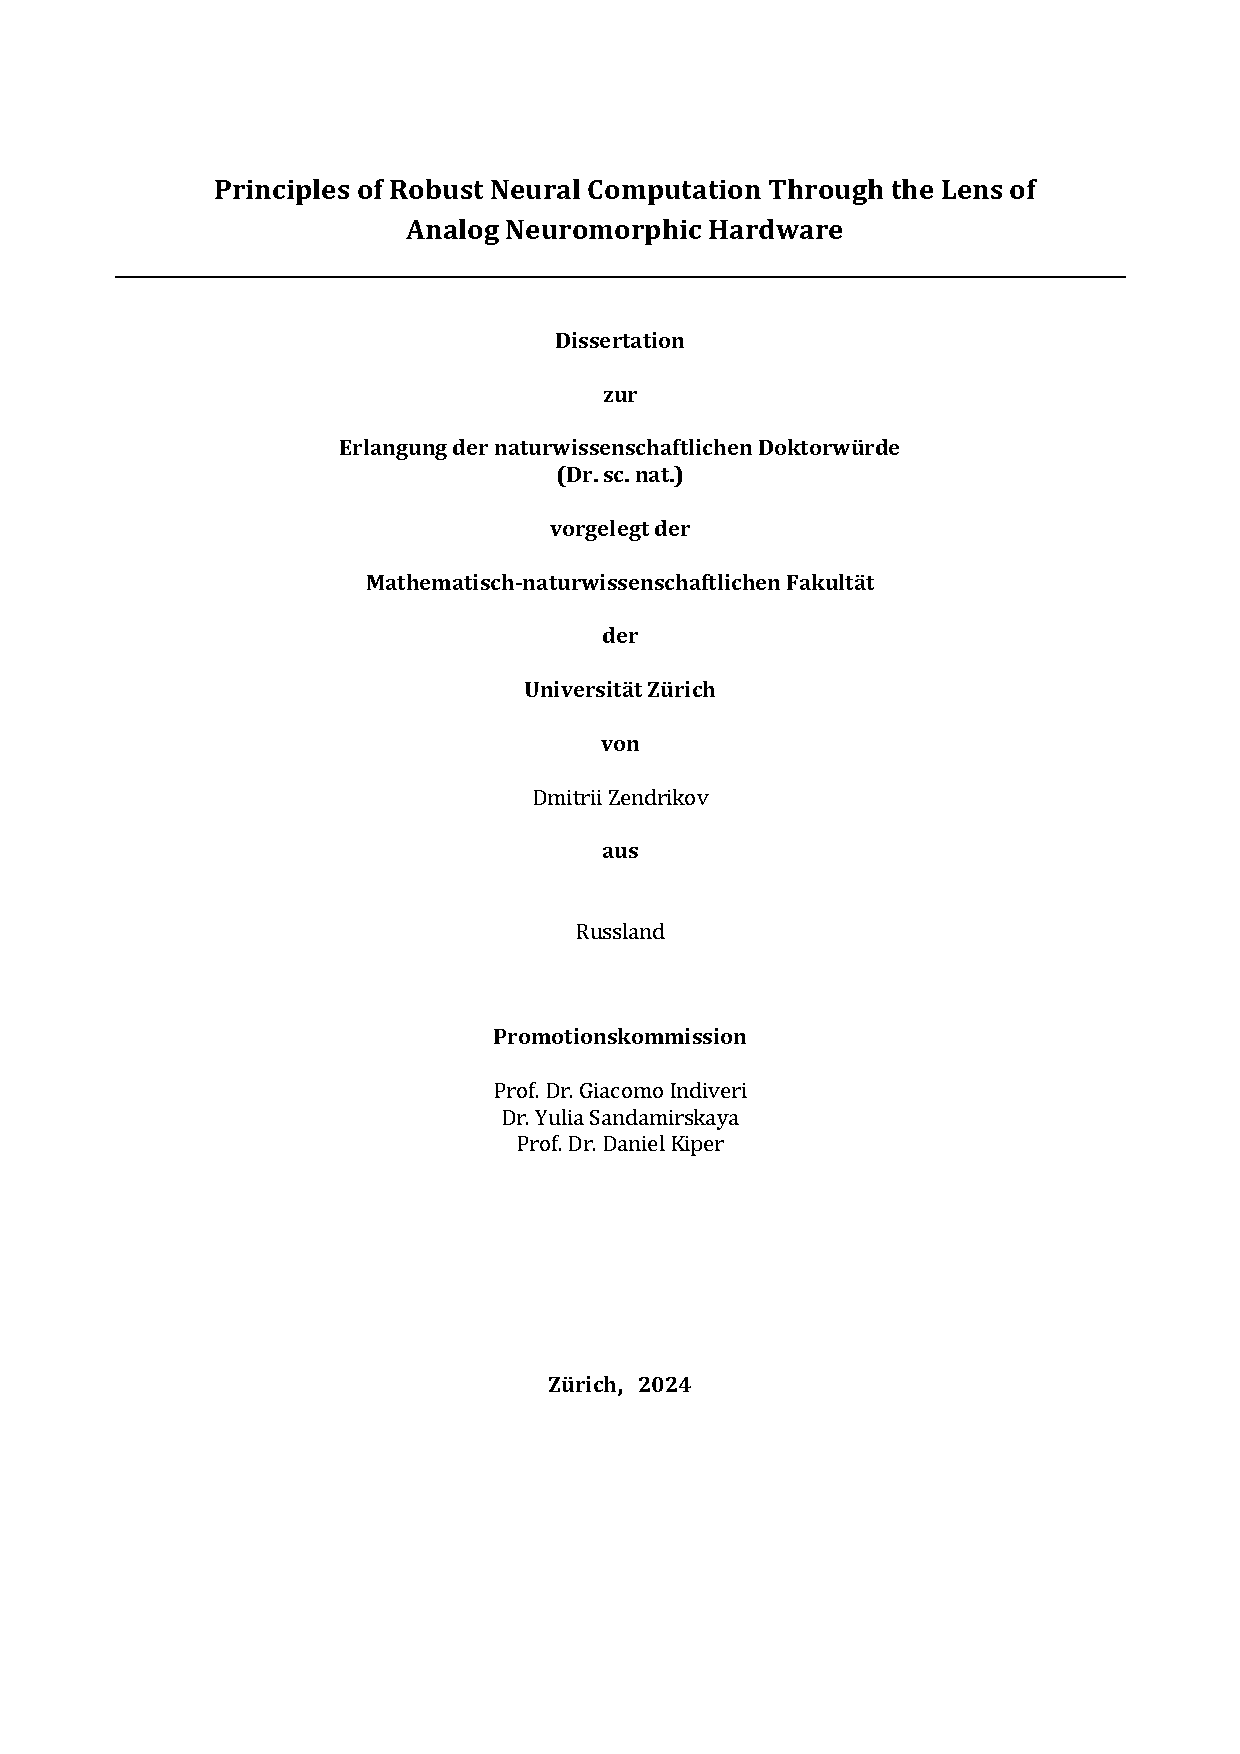
\includepdf[pages=-]{Titelblatt.pdf}
 \setlength{\voffset}{\originalVOffset}
 \setlength{\hoffset}{\originalHOffset}

\maketitle 							% Create title page

\clearpage
\thispagestyle{empty}
\vspace*{\fill}
 
% Preamble_______________________________________________________________

\pagenumbering{roman} 				% Begin roman page numbering (i,ii,...)

%---------------------------------------------------------------------------
% Preface

\chapter*{Abstract}
 \addcontentsline{toc}{chapter}{Abstract}

Neuromorphic electronics provide a computational substrate that natively supports spiking neural networks through device physics, making them strong competitors for low-power edge computing applications. This class of devices is fundamentally different from conventional digital processors, and so is the computation they are capable of.

Development path of this technology is about to reach a new stage, combining multiple domains, like CMOS circuits and memristive or ferroelectric devices, on the same die. To educate the upcoming design choices, it is necessary to build a firm understanding of the advantages and limitations of the current generation of chips, which can be done by systematically extracting the most out of them and identifying missing components for possible applications.

This work represents a bottom-up journey of scientific exploration towards achieving robust neuromorphic computing. Having the dream of autonomous intelligent neuromorphic systems as a distant goal, we define and test computational primitives serving as building blocks for such intelligence. We use a current-generation general-purpose neuromorphic processor to demonstrate the accessibility of computational elements, previously implemented with application-specific circuits. Moreover, since the chip design is inspired by the nervous system at the lowest level, we demonstrate that the brain-derived strategies benefit coding and its robustness at the network level.

Through analysis of individual neuron circuits, small populations and the exploitation of the reprogrammable routing scheme of the chip, we configure multiple network prototypes that implement i) a network of relations, ii) a model of unsupervised cortical map formation, iii) a spatiotemporal pattern classifier and iv) an example of closed-loop neuromorphic agent capable of reinforcement learning.

As a result, we provide tools and insights into how neuromorphic hardware should be approached, showing how such seemingly different domains of computation, in fact, fit well under the umbrella of the same principles of space and time averaging, and introduced stochasticity.


%\dz{DRAFT: Understanding by building is really the epitome of this work. While the tangible global task declared for the project had been to "build neuromorphic agents", it was formulated in a way that fosters bio-inspired methodological search, drastically constraining the field of possible solutions. This work represents the work philosophy and the results of what happens, when instead of paving a high-level path to a problem solution, one would rather focus on low-level details, crossing out some technologies and keeping the others, resulting in a small piece of this "edible pie" in the end, the intersection of all constraints. And only then, having this set of rules declared important, you begin to see what high-level task it would solve. This probably tells the story of a true bottom-up approach, spanning across multiple domains and converging to a functional prototype.}
\newpage
 
\chapter*{Acknowledgements}
\addcontentsline{toc}{chapter}{Acknowledgements}

This work is supported by the EU ERC Grant 'NeuroAgents' (No. 724295)

%\begin{verbatim}
%thesis thanks:
%Giacomo for care, believing in me, and the art of scientific storytelling, the example of
%    passion for the elegance of neuromorphic technology
%my dad and family
%Kathrin and Simone, not only administrative, but emotional support
%Sergio (and Sonia) - for work discussions but also hospitality and good times on Sardinia
%Alexander Paraskevov
%NCS Group
%Nicoletta 
%Eugenia
%Karina
%Veronika 
%Yulia for the inspiration to push and leading by example. And of course aviation
%Hector for making me rebuild my mental health by reintegrating me into zurich music %scene
%Maryada
%Matteo
%Moritz for setting a bar and an example, how to work and how to party. And CapoCaccia and Kafischnaps sessions
%Matthew Cook
%Vanessa (for sparkle and energy)
%Leo for assuming i have all the answers and making me try to live up to expectations
%Ayush
%Alex & UW
%Sasha
%    
%\end{verbatim}
\newpage

%---------------------------------------------------------------------------
% Table of contents

 \setcounter{tocdepth}{2}
 \tableofcontents

 \newpage

%---------------------------------------------------------------------------
% Symbols

\chapter*{Nomenclature}\label{chap:symbole}
 \addcontentsline{toc}{chapter}{Nomenclature}

\section*{Acronyms and Abbreviations}
\begin{acronym}
\acro{ADC}[ADC]{Analog to Digital Converter}
\acro{ADEXP}[AdExp-I\&F]{Adaptive-Exponential Integrate and Fire}
\acro{ADM}[ADM]{Asynchronous Delta Modulator}
\acro{AER}[AER]{Address-Event Representation}
\acro{AEX}[AEX]{AER EXtension board}
\acro{AE}[AE]{Address-Event}
\acro{AFM}[AFM]{Atomic Force Microscope}
\acro{AGC}[AGC]{Automatic Gain Control}
\acro{AI}[AI]{Artificial Intelligence}
\acro{AMDA}[AMDA]{AER Motherboard with D/A converters}
\acro{ANN}[ANN]{Artificial Neural Network}
\acro{API}[API]{Application Programming Interface}
\acro{APMOM}[APMOM]{Alternate Polarity Metal On Metal}
\acro{ARM}[ARM]{Advanced RISC Machine}
\acro{ASIC}[ASIC]{Application Specific Integrated Circuit}
\acro{AdExp}[AdExp-IF]{Adaptive Exponential Integrate-and-Fire}
\acro{BCM}[BMC]{Bienenstock-Cooper-Munro}
\acro{BD}[BD]{Bundled Data}
\acro{BEOL}[BEOL]{Back-end of Line}
\acro{BG}[BG]{Bias Generator}
\acro{BMI}[BMI]{Brain-Machince Interface}
\acro{BTB}[BTB]{band-to-band tunnelling}
\acro{CAD}[CAD]{Computer Aided Design}
\acro{CAM}[CAM]{Content Addressable Memory}
\acro{CAVIAR}[CAVIAR]{Convolution AER Vision Architecture for Real-Time}
\acro{CA}[CA]{Cortical Automaton}
\acro{CCN}[CCN]{Cooperative and Competitive Network}
\acro{CDR}[CDR]{Clock-Data Recovery}
\acro{CFC}[CFC]{Current to Frequency Converter}
\acro{CHP}[CHP]{Communicating Hardware Processes}
\acro{CMIM}[CMIM]{Metal-insulator-metal Capacitor}
\acro{CML}[CML]{Current Mode Logic}
\acro{CMOL}[CMOL]{Hybrid CMOS nanoelectronic circuits}
\acro{CMOS}[CMOS]{Complementary Metal-Oxide-Semiconductor}
\acro{CNN}[CCN]{Convolutional Neural Network}
\acro{COTS}[COTS]{Commercial Off-The-Shelf}
\acro{CPG}[CPG]{Central Pattern Generator}
\acro{CPLD}[CPLD]{Complex Programmable Logic Device}
\acro{CPU}[CPU]{Central Processing Unit}
\acro{CSM}[CSM]{Cortical State Machine}
\acro{CSP}[CSP]{Constraint Satisfaction Problem}
\acro{CTXCTL}[CTXCTL]{CortexControl}
\acro{CV}[CV]{Coefficient of Variation}
\acro{DAC}[DAC]{Digital to Analog Converter}
\acro{DAS}[DAS]{Dynamic Auditory Sensor}
\acro{DAVIS}[DAVIS]{Dynamic and Active Pixel Vision Sensor}
\acro{DBN}[DBN]{Deep Belief Network}
\acro{DFA}[DFA]{Deterministic Finite Automaton}
\acro{DIBL}[DIBL]{drain-induced-barrier-lowering}
\acro{DI}[DI]{delay insensitive}
\acro{DMA}[DMA]{Direct Memory Access}
\acro{DNF}[DNF]{Dynamic Neural Field}
\acro{DNN}[DNN]{Deep Neural Network}
\acro{DOF}[DOF]{Degrees of Freedom}
\acro{DPE}[DPE]{Dynamic Parameter Estimation}
\acro{DPI}[DPI]{Differential Pair Integrator}
\acro{DRAM}[DRAM]{Dynamic Random Access Memory}
\acro{DRRZ}[DR-RZ]{Dual-Rail Return-to-Zero}
\acro{DR}[DR]{Dual Rail}
\acro{DSP}[DSP]{Digital Signal Processor}
\acro{DVS}[DVS]{Dynamic Vision Sensor}
\acro{DYNAP}[DYNAP]{Dynamic Neuromorphic Asynchronous Processor}
\acro{EBL}[EBL]{Electron Beam Lithography}
\acro{EDVAC}[EDVAC]{Electronic Discrete Variable Automatic Computer}
\acro{EEG}[EEG]{electroencephalography}
\acro{EIN}[EIN]{Excitatory-Inhibitory Network}
\acro{EM}[EM]{Expectation Maximization}
\acro{EPSC}[EPSC]{Excitatory Post-Synaptic Current}
\acro{EPSP}[EPSP]{Excitatory Post-Synaptic Potential}
\acro{EZ}[EZ]{Epileptogenic Zone}
\acro{FDSOI}[FDSOI]{Fully-Depleted Silicon on Insulator}
\acro{FET}[FET]{Field-Effect Transistor}
\acro{FFT}[FFT]{Fast Fourier Transform}
\acro{FI}[F-I]{Frequency-Current}
\acro{FPGA}[FPGA]{Field Programmable Gate Array}
\acro{FR}[FR]{Fast Ripple}
\acro{FSA}[FSA]{Finite State Automaton}
\acro{FSM}[FSM]{Finite State Machine}
\acro{GIDL}[GIDL]{gate-induced-drain-leakage}
\acro{GOPS}[GOPS]{Giga-Operations per Second}
\acro{GPU}[GPU]{Graphical Processing Unit}
\acro{GUI}[GUI]{Graphical User Interface}
\acro{HAL}[HAL]{Hardware Abstraction Layer}
\acro{HFO}[HFO]{High Frequency Oscillation}
\acro{HH}[H\&H]{Hodgkin \& Huxley}
\acro{HMM}[HMM]{Hidden Markov Model}
\acro{HRS}[HRS]{High-Resistive State}
\acro{HR}[HR]{Human Readable}
\acro{HSE}[HSE]{Handshaking Expansion}
\acro{HW}[HW]{Hardware}
\acro{ICT}[ICT]{Information and Communication Technology}
\acro{IC}[IC]{Integrated Circuit}
\acro{IEEG}[iEEG]{intracranial electroencephalography}
\acro{IF2DWTA}[IF2DWTA]{Integrate \& Fire 2--Dimensional WTA}
\acro{IFSLWTA}[IFSLWTA]{Integrate \& Fire Stop Learning WTA}
\acro{IF}[I\&F]{Integrate-and-Fire}
\acro{IMU}[IMU]{Inertial Measurement Unit}
\acro{INCF}[INCF]{International Neuroinformatics Coordinating Facility}
\acro{INI}[INI]{Institute of Neuroinformatics}
\acro{IO}[I/O]{Input/Output}
\acro{IPSC}[IPSC]{Inhibitory Post-Synaptic Current}
\acro{IPSP}[IPSP]{Inhibitory Post-Synaptic Potential}
\acro{IP}[IP]{Intellectual Property}
\acro{ISI}[ISI]{Inter-Spike Interval}
\acro{IoT}[IoT]{Internet of Things}
\acro{JFLAP}[JFLAP]{Java - Formal Languages and Automata Package}
\acro{LEDR}[LEDR]{Level-Encoded Dual-Rail}
\acro{LFP}[LFP]{Local Field Potential}
\acro{LLC}[LLC]{Low Leakage Cell}
\acro{LNA}[LNA]{Low-Noise Amplifier}
\acro{LPF}[LPF]{Low Pass Filter}
\acro{LRS}[LRS]{Low-Resistive State}
\acro{LSM}[LSM]{Liquid State Machine}
\acro{LTD}[LTD]{Long Term Depression}
\acro{LTI}[LTI]{Linear Time-Invariant}
\acro{LTP}[LTP]{Long Term Potentiation}
\acro{LTU}[LTU]{Linear Threshold Unit}
\acro{LUT}[LUT]{Look-Up Table}
\acro{LVDS}[LVDS]{Low Voltage Differential Signaling}
\acro{MCMC}[MCMC]{Markov-Chain Monte Carlo}
\acro{MEMS}[MEMS]{Micro Electro Mechanical System}
\acro{MFR}[MFR]{Mean Firing Rate}
\acro{MIM}[MIM]{Metal Insulator Metal}
\acro{MLP}[MLP]{Multilayer Perceptron}
\acro{MOSCAP}[MOSCAP]{Metal Oxide Semiconductor Capacitor}
\acro{MOSFET}[MOSFET]{Metal Oxide Semiconductor Field-Effect Transistor}
\acro{MOS}[MOS]{Metal Oxide Semiconductor}
\acro{MRI}[MRI]{Magnetic Resonance Imaging}
\acro{NDFSM}[NDFSM]{Non-deterministic Finite State Machine} 
\acro{ND}[ND]{Noise-Driven}
\acro{NEF}[NEF]{Neural Engineering Framework}
\acro{NHML}[NHML]{Neuromorphic Hardware Mark-up Language}
\acro{NIL}[NIL]{Nano-Imprint Lithography}
\acro{NMDA}[NMDA]{N-Methyl-D-Aspartate}
\acro{NME}[NE]{Neuromorphic Engineering}
\acro{NN}[NN]{Neural Network}
\acro{NOC}[NoC]{Network-on-Chip}
\acro{NRZ}[NRZ]{Non-Return-to-Zero}
\acro{NSM}[NSM]{Neural State Machine}
\acro{OR}[OR]{Operating Room}
\acro{OTA}[OTA]{Operational Transconductance Amplifier}
\acro{PCB}[PCB]{Printed Circuit Board}
\acro{PCHB}[PCHB]{Pre-Charge Half-Buffer}
\acro{PCM}[PCM]{Phase Change Memory}
\acro{PE}[PE]{Phase Encoding}
\acro{PFA}[PFA]{Probabilistic Finite Automaton}
\acro{PFC}[PFC]{prefrontal cortex}
\acro{PFM}[PFM]{Pulse Frequency Modulation}
\acro{PR}[PR]{Production Rule}
\acro{PSC}[PSC]{Post-Synaptic Current}
\acro{PSP}[PSP]{Post-Synaptic Potential}
\acro{PSTH}[PSTH]{Peri-Stimulus Time Histogram}
\acro{QDI}[QDI]{Quasi Delay Insensitive}
\acro{RAM}[RAM]{Random Access Memory}
\acro{RA}[RA]{Resected Area}
\acro{RDF}[RDF]{random dopant fluctuation}
\acro{RELU}[ReLu]{Rectified Linear Unit}
\acro{RLS}[RLS]{Recursive Least-Squares}
\acro{RMSE}[RMSE]{Root Mean Squared-Error}
\acro{RMS}[RMS]{Root Mean Squared}
\acro{RNN}[RNN]{Recurrent Neural Networks}
\acro{ROLLS}[ROLLS]{Reconfigurable On-Line Learning Spiking}
\acro{RRAM}[R-RAM]{Resistive Random Access Memory}
\acro{R}[R]{Ripples}
\acro{SAC}[SAC]{Selective Attention Chip}
\acro{SAT}[SAT]{Boolean Satisfiability Problem}
\acro{SCX}[SCX]{Silicon CorteX}
\acro{SD}[SD]{Signal-Driven}
\acro{SEM}[SEM]{Spike-based Expectation Maximization}
\acro{SLAM}[SLAM]{Simultaneous Localization and Mapping}
\acro{SNN}[SNN]{Spiking Neural Network}
\acro{SNR}[SNR]{Signal to Noise Ratio}
\acro{SOC}[SOC]{System-On-Chip}
\acro{SOI}[SOI]{Silicon on Insulator}
\acro{SOZ}[SOZ]{Seizure Onset Zone}
\acro{SP}[SP]{Separation Property}
\acro{SRAM}[SRAM]{Static Random Access Memory}
\acro{STDP}[STDP]{Spike-Timing Dependent Plasticity}
\acro{STD}[STD]{Short-Term Depression}
\acro{STP}[STP]{Short-Term Plasticity}
\acro{STT-MRAM}[STT-MRAM]{Spin-Transfer Torque Magnetic Random Access Memory}
\acro{STT}[STT]{Spin-Transfer Torque}
\acro{SW}[SW]{Software}
\acro{TCAM}[TCAM]{Ternary Content-Addressable Memory}
\acro{TFT}[TFT]{Thin Film Transistor}
\acro{TLE}[TLE]{Temporal Lobe Epilepsy}
\acro{USB}[USB]{Universal Serial Bus}
\acro{VHDL}[VHDL]{VHSIC Hardware Description Language}
\acro{VLSI}[VLSI]{Very Large Scale Integration}
\acro{VOR}[VOR]{Vestibulo-Ocular Reflex}
\acro{WCST}[WCST]{Wisconsin Card Sorting Test}
\acro{WTA}[WTA]{Winner-Take-All}
\acro{XML}[XML]{eXtensible Mark-up Language}
\acro{divmod3}[DIVMOD3]{divisibility of a number by three}
\acro{hWTA}[hWTA]{hard Winner-Take-All}
\acro{sWTA}[sWTA]{soft Winner-Take-All}
\end{acronym}



 \newpage

%---------------------------------------------------------------------------


\pagestyle{fancy}               	% Fancy headings
\pagenumbering{arabic}				% Begin arabic page numbering (1,2,...)


% Chapters______________________________________________________________________
\renewcommand\sectionbreak{} 
\chapter{Introduction}
\label{chapter:introduction}

%\subsection{Thesis Objectives}
\section{Thesis Outline}

\subsection{Making neuromorphic hardware more accessible(??)}

\newpage

%\renewcommand{\sectionbreak}{\clearpage}
\chapter{Understanding before building. Variability in analog subthreshold circuits.}
\label{ch:introduction_to_hardware}

The story begins with single spiking neurons and emulation of their behaviour through \ac{MOSFET} transistor physics~\cite{Chicca_etal14}. Before we begin connecitng neurons together, it is essential to have this bottom-layer block well-defined. When implemented in hardware, these circuits are much harder to characterize compared to mathematical models, so let us start with the definition of the spiking neuron model we use. This also will be useful later as we attempt to align the physical neurons with their simulated prototypes and begin seeing the device-induced variability in the behaviour of the similarly tuned silicon neurons.

%With the goal of understanding the brain function through reproduction and knowing that computation is done with networks of these units, it is essential to have this bottom-layer block well-defined. A number of spiking neuron models have been developed with varying levels of complexity and types of biologically relevant behaviour~\cite{Izhikevich04}. Typically, the more complex the model, the more elaborate the dynamics of the real cells it reflects at the cost of additional computational resources. And by resources, one can see not only the calculation steps it takes to solve systems of differential equations but also the physical area it would take to emulate such neuron behaviour with an analog circuit.


\section{Modeling a leaky integrate-and-fire neuron}

Leaky integrate-and-fire (LIF) spiking neuron model is a commonly selected trade-off between biological plausibility and computational complexity. It captures the most essential properties of the biological neurons while remaining fairly accessible for mathematical analysis. LIF neurons are often used in numerical simulations of various SNNs, and are also implemented as transistor circuits on hardware (see the next Section).

From computational neuroscience, the defining behaviour of neuron cells is their ability to integrate electrical pulses (spikes) from dendrites (inputs) and generate action potentials down their axons (outputs) onwards to other neurons.
In neuroinformatics, this is described by different mathematical models with a wide variety of depth and detail~\cite{Izhikevich04}. A common approach is a description of the neuron as a point (i.e. not modelling cell body geometry) and using its membrane potential (or transmembrane voltage) $V_{mem}(t)$ as its state variable.

An optimal trade-off between biological plausibility, computational complexity and analytical interpretability is often seen in the \ac{LIF} neuron model.

\begin{eqnarray}
    \tau_m \frac{dV_{mem}(t)}{dt} & = & - (V_{mem}(t) - V_{rest}) + RI_{in}(t) \label{eq:LIF}\\
    V_{mem}(t) > V_{th} & \rightarrow & V_{mem}(t) = V_{reset}, t^i_{sp} = t
    \label{eq:LIF_reset}
\end{eqnarray}

where in absence of input currents $I_{in}(t)$ though the membrane with conductance $R$, the membrane voltage $V_{mem}$ would decay exponentially to the resting potential $V_{rest}$ with the time constant $\tau_{m}$. The neuron emits a spike if $V_{mem}(t)$ exceeds a threshold value $V_{th}$. In that case, the moment of crossing the threshold $t_{sp}$ is recorded and $V_{mem}(t)$ is reset to $V_{reset}$ for the duration of a refractory period $\tau_{ref}$, after which the dynamics of $V$ is again described by Equation~\ref{eq:LIF}.

With the addition of the spike frequency adaptation and the exponential positive feedback modeling the sodium channels, we get the \ac{ADEXP-LIF} neuron model ~\cite{Brette_Gerstner05} that will be referenced throughout the rest of the work, which in its generalized form is:

\begin{eqnarray}
    \tau_{mem} \frac{dV_{mem}}{dt} & = & - (V_{mem}(t) - V_{rest}) - V_{th}(t) + f(V_{mem}) + R_{m}I_{in}(t)     \label{eq:AdEx}\\
    \tau_{adapt}\frac{dV_{th}(t)}{dt} & = &  -V_{th}(t) + A_{adapt} \delta(t-t_{sp}) \label{eq:LIF_adaptation}\\
    V_{mem}(t) > V_{th} & \rightarrow & V(t) = V_{reset}, t^i_{sp} = t
\end{eqnarray}

where the $f(V_{mem})$ is the exponential positive feedback term, and $V_{th}$ has its own decaying dynamics, increasing with every spike the neuron emits, providing negative feedback for $V_{mem}$ (i.e. decreasing excitability). The incoming spikes (emitted by the neuron itself, in this case) at time $t^i_{sp}$ are commonly modeled as delta-functions~\cite{Dayan_Abbott01}.

The input to the neuron is provided through the input current, a sum of the pulses through connections (synapses) coming from the other neurons and the direct input current that could be injected externally:

\begin{equation}
    I_{in}(t) = \sum_{j}I^{ij}_{syn}(t) + I_{dc}(t)
    \label{eq:I_in}
\end{equation}

Synaptic currents are commonly modeled as exponentially relaxating as well, with spikes from other neurons $j$ arriving to the neuron $i$ at times $t^{ij}_{syn}$:

\begin{equation}
    \tau_{syn}\frac{dI_{syn}(t)}{dt} = -I_{syn}(t) + \sum_{j}\delta(t - t^{ij}_{syn}(t))
    \label{eq:I_syn}
\end{equation}

The set of equations above defines neuronal and synaptic transmission. To utilize them within an embedded setting, there has to be some hardware system that does the numerical calculation of these models.
Here, two approaches are possible: digital simulation or emulation by some other physical process.
In the first case, an iterative solver would numerically solve the equations, for example, using Euler or RK3-RK4~\cite{Butcher96, Brette_etal07} methods. The accuracy of the solution would depend on the method and the timestep size of the solver. Typically, since the described model does not have any stochasticity, the results of the simulation would also be deterministic and thus precisely reproducible, which is ideal for any studies of neural network dynamics and its changes created by any smallest perturbations. The drawback of this approach is the computational load that builds up with the number of neurons and synapses simulated simultaneously, as well as with the precision of the numerical solution. This is where classical von Neumann architecture becomes a limiting factor, imposing constraints on the scale of the network, simulation speed relative to real-time, and energy consumption.

The alternative to numerical simulation is direct hardware \emph{emulation}.

\section{Silicon neurons of the DYNAP-SE1 chip}

%\subsection{The computational substrate. Introducing the neurons of DYNAP-SE1.}


For the second approach, the solutions of the equations are \emph{emulated} directly by the electrical circuits. %Exploiting the property of the \ac{MOSFET} transistors, where below the source-to-gate threshold, the diffusion current through the transistor depends exponentially on the gate voltage \dz{which is a nightmare for a traditional electrical engineer OR ADD THIS TO SECTION DISCUSSION}

%\begin{equation}
%    I = I_0 e^{\frac{-V}{\kappa U_t}}
%\end{equation}

%with $\kappa$ and $U_t$ being constant material properties \dz{OF? TBA},
As a result, a circuit of a DPI \ac{ADEXP-LIF} neuron can be constructed~\cite{Livi_Indiveri09, Chicca_etal14}, as illustrated in Figure~\ref{fig:DPI_neuron_and_synapse}.

\begin{figure}[h]
    \centering
    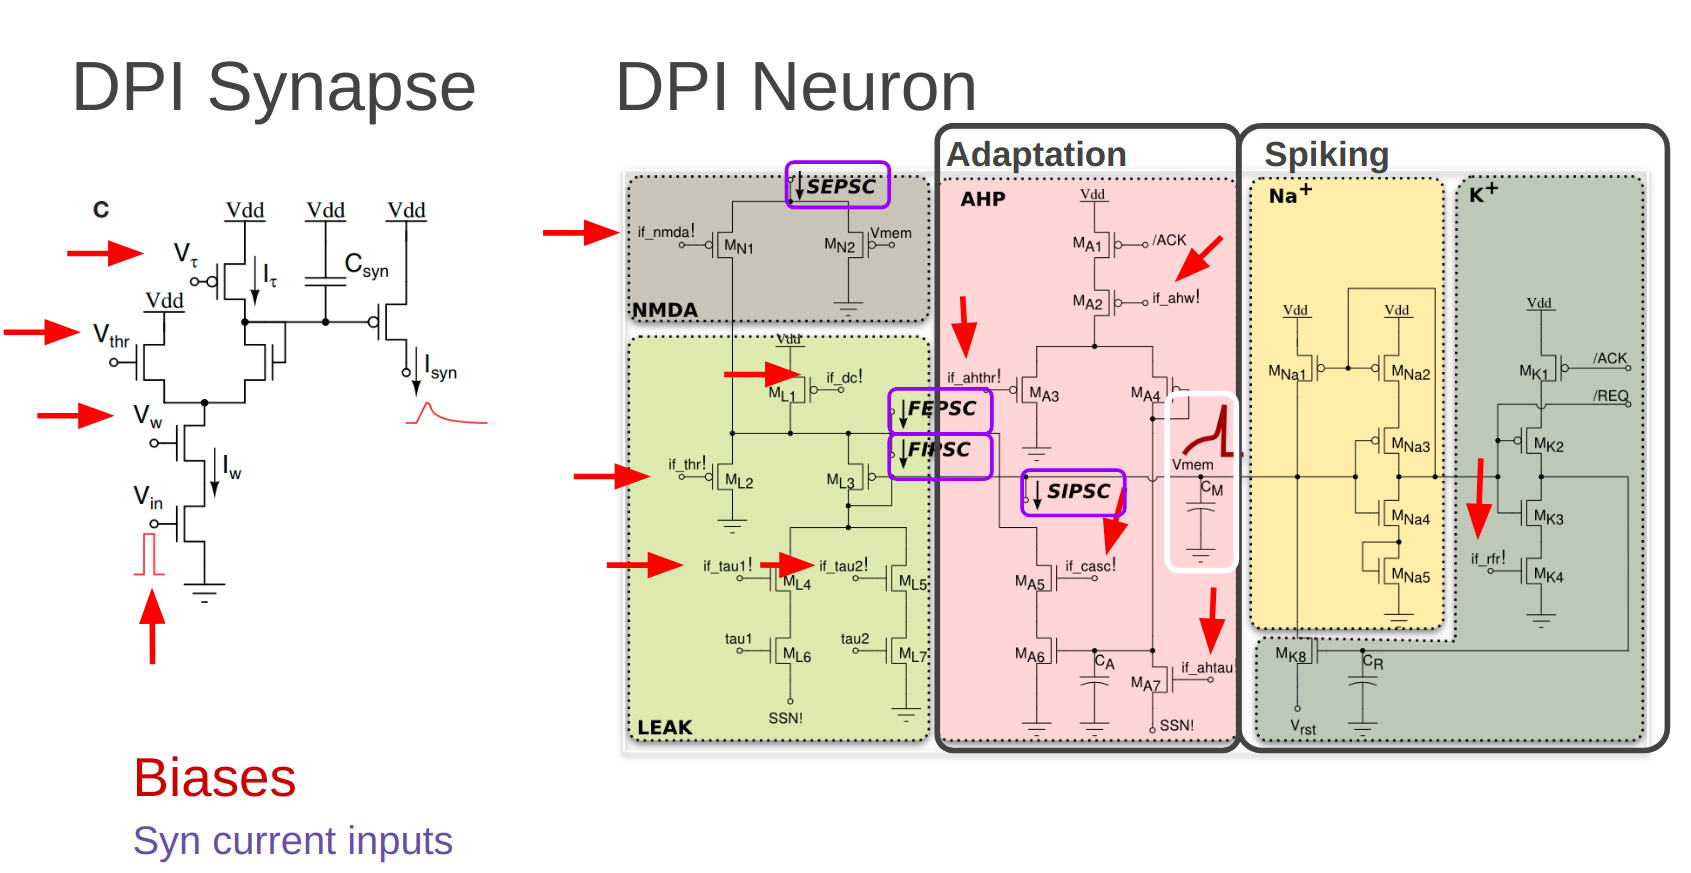
\includegraphics[width=\textwidth]{img/chapter4/DPI_neuron_and_synapse.png}
    \caption[Schematics of circuits of a DPI \ac{ADEXP-LIF} neuron and a DPI alpha synapse]{Schematics of circuits of a DPI \ac{ADEXP-LIF} neuron and a DPI alpha synapse, adapted from~\cite{Chicca_etal14, Livi_Indiveri09}. All transistors are operated in the subthreshold regime, with circuits emulating the synaptic current and the voltage shape on their output nodes, respectively. Red arrows highlight gate voltages controlling behaviour properties of the neuron and the synapse, such as the time constants, refractory period or synaptic weights.}
    \label{fig:DPI_neuron_and_synapse}
\end{figure}

Within these circuits, all neuron and synapse parameters are controlled by gate voltages, or biases, on specific transistors (highlighted in red).

%\dz{TBA: about current-based emulation of parameters? to link to the equations in the next chapter?}

Following~\cite{Chicca_etal14}, the neuron circuit shown in Figure~\ref{fig:DPI_neuron_and_synapse} gives a current-based differential equation, following the form of the original \ac{ADEXP-LIF} neuron Equation~\ref{eq:AdEx} with a few extra terms, but with the membrane voltage of the model is emulated by a current $I_{mem}$: %\dz{TBA: label nodes in the figure, add $GABA_a$ current to the equation.}

\begin{eqnarray}
    \left(1+\frac{I_g}{I_{mem}}\right)\tau_m\frac{dI_{mem}}{dt}&=&-I_{mem} \left( 1+\frac{I_{ahp}}{I_\tau} \right) + \frac{I_g}{I_{\tau}}(I_{in} - I_{ahp} - I_{\tau}) + f(I_{mem})
    \label{eq:dynapse_LIF}\\
    \tau_m & \triangleq & \frac{CU_t}{\kappa I_{\tau}}
    \label{eq:dynapse_LIF_TC}
\end{eqnarray}

where $I_{mem}$ is the state variable representing the membrane potential; $I_{ahp}$ is the firing threshold adaptation current behaving similarly to Eq.~\ref{eq:LIF_adaptation}; $I_{g}$ is the DPI gain current; $\tau_{m}$ is the time constant inversely proportional to the leak current $I_{\tau}$; $f(I_{mem})$ is the positive exponential feedback term and $I_{in}$ is the total input current. The currents $I_{g}$ and $I_{\tau}$ are directly controlled by the respective constant voltage biases \verb|if_thr!| and \verb|if_tau1!|, other biases are also constant but applied indirectly.

If the DPI gain $I_{g}$ is low, the equation can be further simplified under the assumption that $I_{g} \ll I_{mem}$ which brings it closer to the original mathematical model:

\begin{eqnarray}
    \tau_m\frac{dI_{mem}}{dt}&=&-I_{mem} + \frac{I_g}{I_{\tau}}I_{in} + f(I_{mem})\\
    \label{eq:dynapse_LIF}
\end{eqnarray}

\begin{figure}[h]
  \centering
  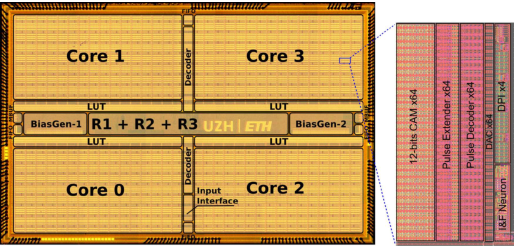
\includegraphics[width=0.75\textwidth]{img/chapter4/chip-dynap-se-pixel.pdf}
  \caption[Die photo of the DYNAP-SE multi-core neuromorphic processor]{Die photo of the DYNAP-SE multi-core neuromorphic processor, with single neuron element highlighted.
The chip was fabricated using a standard 0.18\,$\mu m$ 1P6M \ac{CMOS} technology.
Neurons between cores and between different chips can be interconnected by programming the on-chip CAM memory cells and the asynchronous digital routers labelled R1, R2, and R3.
The circuit parameters can be set independently for each core using on-chip 12\,bit bias generators. Figure adapted from~\cite{Moradi_etal18}.}
  \label{fig:dynapse}
\end{figure}


A circuit producing the synaptic current $I_{syn}$ (also presented in~\cite{Chicca_etal14}) has a similar, albeit simpler (without having the spike generation mechanism) structure, consisting of a pFET DPI, the main capacitor representing the state of the synapse (fully charged meaning there is no synaptic current), the leakage current $I_{\tau_{syn}}$ controlling the synaptic pulse relaxation, and a spike processing branch producing an instantaneous change to the capacitor voltage with the current $I_w$ with fixed amplitude, modelling the synaptic weight, whenever an input event opens the $V_{in}$ gate. The equation for $I_{syn}$ derived from the circuit (Figure~\ref{fig:DPI_neuron_and_synapse} left) is the following:

\begin{eqnarray}
    \tau_{syn}\frac{dI_{syn}}{dt}&=&-I_{syn}+\frac{I^{syn}_{g}}{I_\tau} I_w
    \label{eq:DPI_synapse}
\end{eqnarray}

where $I^{syn}_{g}$ is the \ac{DPI} threshold of the synapse circuit, or the synaptic current gain.

Utilizing these circuit designs, a \ac{DYNAP}-SE1 chip had been created~\cite{Moradi_etal18}, containing 1024 of these silicon neurons placed on the same die (see Fig.~\ref{fig:dynapse}), allowing the circuits to emulate neuronal dynamics completely independently for all neurons, achieving ultimate asynchronous parallelism. 

On this chip, every neuron has 4 synapse circuits attached to the neuron circuit, implementing 4 different synapse types by injecting or subtracting synaptic currents from the neuron at various points (marked in purple on the neuron circuit in Figure~\ref{fig:DPI_neuron_and_synapse}). The FEPSC ("fast excitatory postsynaptic current") and FIPSC nodes are the "fast" excitatory ($AMPA$) and inhibitory ($GABA_B$) synapses, modelling additive and subtractive (dendritic) synaptic inputs, respectively. The SEPSC ("slow" EPSC) is connected through an extra \ac{DPI} circuit, enabling the $NMDA$ voltage gating. Without the $NMDA$ bias (shown as \verb|if_nmda!| in Fig.~\ref{fig:DPI_neuron_and_synapse}), this synapse functions identically to $AMPA$, allowing having two excitatory synapse types for the neuron with individual parameter control (as the biases for each neuron and synapse are shared across the core for bias generator chip area reasons, as discussed before). Finally, the SIPSC (or $GABA_A$) node is the somatic inhibition, subtracting charge directly from the neuron capacitor.

The implemented architecture allows direct monitoring of the neuron's capacitor voltage $V_{mem}$ with the oscilloscope, allowing probing of individual neurons, which is heavily utilized throughout this work.

\newpage
\section{The precise, the hidden and the complex. The Triangle of uncertain relations (between model, hardware and chip-derived neuron implementations)}
\label{subsec:triangle_of_relations}

Having discussed the details of the mathematical neuron models and the silicon circuits that implement them, we arrive at the problem of configuring the neuron parameters to produce consistent behaviour across the domains (as illustrated in Figure~\ref{fig:triangle_of_relations}).

\begin{figure}[h]
  \centering
  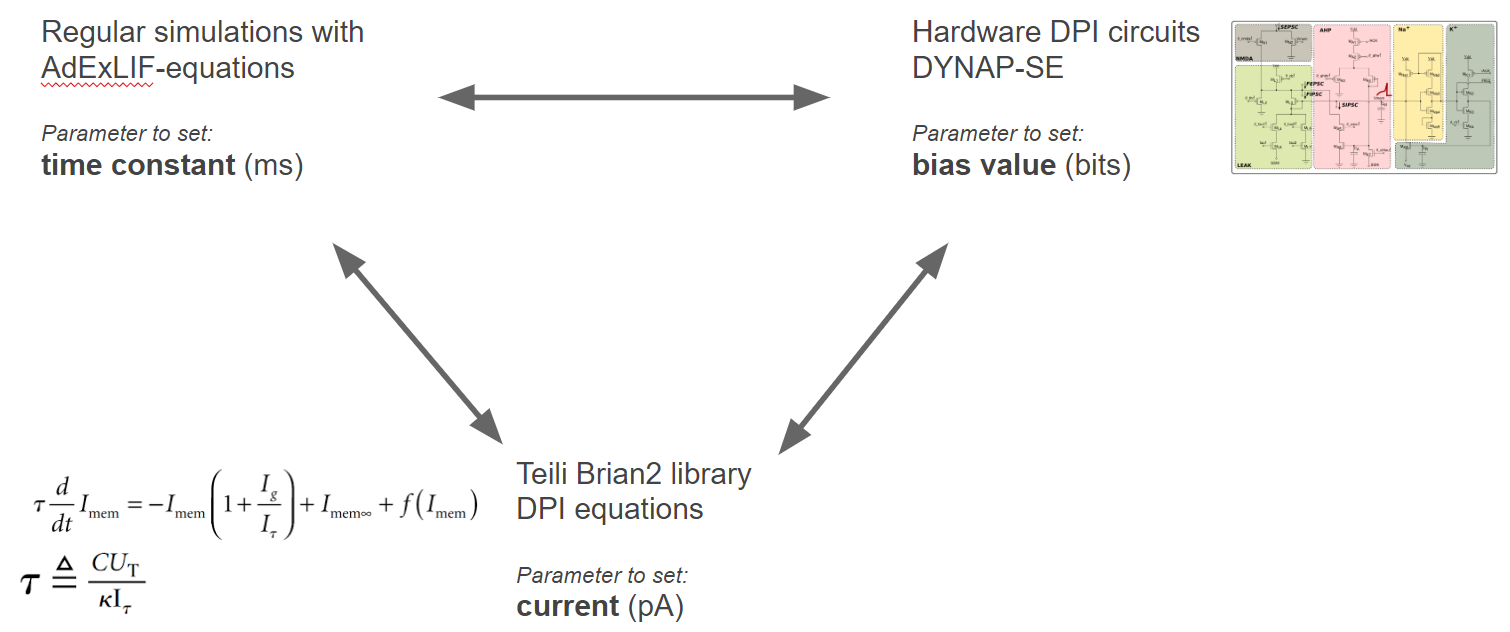
\includegraphics[width=.9\textwidth]{img/chapter4/Triangle_of_uncertainty.png}
  \caption[The problem of mapping between the three domains of modeling spiking neuron dynamics.]{The problem of mapping parameters between the three domains of modeling spiking neuron dynamics: (i) the simulation of the true AdExLIF neuron equations, (ii) the hardware silicon neuron and (iii) the circuit-derived silicon neuron equations~\cite{Milde_etal18}. For the example of a neuron time constant, in all three cases the parameters to set a different: the time constant in units of time, the bit string for the bias generator or the leakage current, respectively. While the link between the two types of simulations can be bridged by approximating the time constant from the transistor equation, a mapping the hardware is impossible to define due to unobservable variability of not only neuron circuits but also the bias generators.}
  \label{fig:triangle_of_relations}
\end{figure}

For the example of the neuron time constant, in numerical simulations of Equation~\ref{eq:AdEx} it is directly set as a parameter $\tau_m$ in the units of time, while for the case of the on-chip current-based DPI neuron circuit, the value controlling the neuron time constant is an abstract \emph{bias value} that is interpreted by the bias generator block, that in turn controls the membrane leakage current.
And completely apart from the two, in a numerical simulation package~\cite{Milde_etal18}that uses the hardware-derived equation (Eq.~\ref{eq:dynapse_LIF}), the time constant is set by the value of the leakage current in pA directly.

To connect the three domains together, there needs to be a precise calculation of a bias current produced by the bias generator on hardware and the corresponding calculation of a resulting neuron parameter. This mapping is, in fact, a big challenge to define, as the bias generator circuit itself is a subthreshold circuit~\cite{Delbruck_etal10} is subject to silicon variability, and the real bias current on the chip cannot be measured directly.

The DPI neuron Equation~\ref{eq:dynapse_LIF} sits in the middle of the three in terms of the neuron dynamics complexity: it has more nonlinear interdependent variables compared to \ac{ADEXP-LIF} Eq.~\ref{eq:AdEx}, but is itself only an approximation of the physical processes happening in the silicon circuit (i.e. not capturing the effects when certain transistors go in/out of saturation).

The strategy we use to bridge the simulation and the emulation domains closer together is the measurement and the response waveform analysis of the silicon neurons through the only available analog state parameter $V_{mem}$. Through such measurement automation we can build the maps between the bias values and the parameters set to the circuit. The same can be done by fitting the simulation traces to confirm the proportionality factor of the Equation~\ref{eq:dynapse_LIF_TC}. But before we do that, however, we need to address the built-in variability of the subthreshold silicon circuits, as the same bias value results an in a distribution of the on-chip neuron behaviours.

%\subsection{Subthreshold circuits. Simulation and emulation.}

%\dz{REWRITE:  is truly a beautiful invention. It gave rise to the entire industry of digital computation as a space- and energy-efficient logic gate, and it kept on giving.}\\

%This section gives a brief and work-relevant introduction of the \emph{neuromorphic engineering} field, the approach of utilizing the physics of subthreshold analog \ac{CMOS} circuits to directly emulate the bio-physics of spiking neurons and synapses through device physics~\cite{Mead90,Mead20}. In conventional electronics, \ac{MOSFET} transistors are normally considered ``closed'' with gate voltage below threshold, as no drift current goes through the channel. The diffusion current that remains if the gate voltage is not equal to the source voltage is usually disregarded, as it depends exponentially on the gate voltage and covers multiple orders of magnitude, which is extremely hard to work with.
%However, exactly this subthreshold behaviour of transistors arranged in a differential pair inspired the association with modeled conductances through the squid neuron cell membrane~\cite{Hodgkin_Huxley52} to create the first silicon neuron circuit~\cite{Mahowald_Douglas91}.

%This idea of emulating mechanisms of one domain by similarly behaving physical properties in the other could be seen as the initial spark, the ground-laying block of the bottom-up ``understanding by building'' approach, where the computation done by biological systems could be studied through reproduction. Having drawn the parallels between exponential behaviour in biophysical processes and diffusion current, the first \emph{neuromorphs} began building circuits emulating the behaviour of the biological counterparts.\\





%\dz{TBA: Add recording for all synapse type shapes here? sharing the synaptic parameters?}

%The communication between the neurons is done via a digital asynchronous hierarchical router~\cite{Moradi_etal18}, with reprogrammable \ac{CAM} and \ac{SRAM} cell located directly at individual neuron circuits, making the \ac{DYNAP}-SE1 chip fulfill the definition of a non-von Neumann mixed-signal processor with truly asynchronous in-memory computing.



%The connectivity solution on this chip is digital but event-driven, meaning that a spike generated by a neuron is immediately picked up by the router \dz{(as soon as it's free to receive an event)~\cite{Moradi_etal18}} and transferred to its postsynaptic neurons based on the reprogrammable \ac{LUT} (i.e. the connectivity matrix), where those events trigger analog current pulses at the input nodes of the synapse circuits.
%This architecture allows to have an efficient, fully parallel real-time emulation of dynamics of a network of \ac{ADEXP-LIF} with a completely flexible connectivity while also \dz{enjoying} the low power consumption aspect of the subthreshold circuits.
%\dz{THIS SECTION NEEDS VERIFICATION FROM THE ROUTING PAPER} The trade-off one faces here is the management of the on-chip surface area. The most area is always taken by capacitors and memory \dz{CHECK THIS}. The decentralized \dz{IS IT?} routing scheme occupies a significant amount of space (around 30\% of the full neuron cell), which is comparable to the area taken by the neuron circuit itself, limiting the fan-out and fan-in of the neuron cells, and thus the reconfigurability of networks the chip can emulate. Another area-induced constraint is the shared parameter setting between the circuits. The bias generators take up a considerable chip area, so in the \ac{DYNAP-SE1} chip design, the bias currents are applied to all 256 neuron cells of a core.



\section{Mismatch and variability in analog neuron circuits. A biological approach to hardware characterization.}

%\dz{This section is adapted from Section 2.2 published in the paper~\cite{Zendrikov_etal23}}.

Having discussed the basics of the neuromorphic circuits we operate with, we need to explore the two other properties inherent to this class of devices.

One is the variations in silicon doping or mismatched geometries intrinsic to the fabrication process of \ac{CMOS} devices~\cite{Pelgrom_etal89} which because of the very low currents (and therefore high sensitivity to such device mismatch) yields heterogeneous electrical properties. These heterogeneous properties affect the behaviour of the analog circuits, even if they have identical geometries at design time.

This factor is central to analog neuromorphic systems, so the computational design built on top has to handle it natively. In the sections below, we discuss the strategies to cope with variability, but first, we build the tools to characterize its scale and behaviour and facilitate the tuning process.

Another property is the parameter configuration flexibility constraints the chip designers have to introduce as a result of optimising the chip area utilization. While the reconfigurable address memory for communication of the neurons is decentralized, it still occupies more than 30\% of the area~\cite{Moradi_etal18}, meaning a limit on the possible fan-in had to be introduced at some level (this is discussed in greater detail in Chapter 4, when we begin connecting neurons together and face that limit). The other significant constraint due to area saving is the bias generator sharing. The bias generator circuits consist of many transistors~\cite{Delbruck_etal10}, so the biasing current has to be shared between groups of neurons. In the case of this chip, every bias is shared between all 256 neurons of a \ac{DYNAP}-SE1 core.

The framework described below aims to automate and systematically configure the \ac{DYNAP}-SE1 chip parameters, while trying to create a methodology general enough to make it transferable to other analog chips utilizing the same circuit design~\cite{Qiao_etal15, Richter_etal24}.


\subsection{Waveform capture and analysis}

To quantify the device mismatch effects in the DYNAP-SE1 circuits accurately, we first defined a set of shared parameters that produce the desired average neuron and synapse behaviours and then systematically measured the circuit responses across all synapse and neuron circuits integrated on the chip.
We automated the data acquisition process using a computer-controlled oscilloscope (see \pyobject{PyScope} in Appendix~\ref{appendix:pyscope}) and measured the analog subthreshold membrane response of the neuron in response to different types of inputs (see the capture and analysis package~\pyobject{BiasTuner} in Appendix~\ref{appendix:bias_tuning_tools}).
We recorded all the measurements on a work-station and carried out standard signal analysis routines to derive the neuron refractory period, the neuron time constant, the synaptic weight and the synaptic time constant from the recordings (see Fig.~\ref{fig:automated_acquisition}).


The refractory period of individual neurons was measured by driving the neuron to produce regular spikes trains with constant input currents, as depicted in Fig.~\ref{fig:neuron_ref}.
The refractory period was defined as the time interval between the action potential reset and the voltage of the neuron rising above the 20\% of its value at rest.

The neuron's time constant was estimated by fitting its response to a step input current small enough to keep the neuron's membrane potential below its firing threshold.
The fit was performed for the decaying part of the circuit response, corresponding to the removal of the input current (see Fig.~\ref{fig:neuron_TC}).

\begin{figure}[h]
  \begin{subfigure}[b]{.3\textwidth}
  \centering
  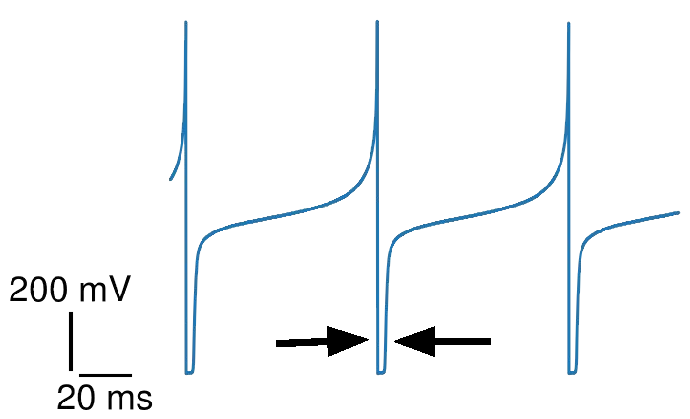
\includegraphics[width=\textwidth]{img/chapter4/neuron_ref.pdf}
  \subcaption{}
  \label{fig:neuron_ref}
  \end{subfigure}
  \begin{subfigure}[b]{.34\textwidth}
  \centering
  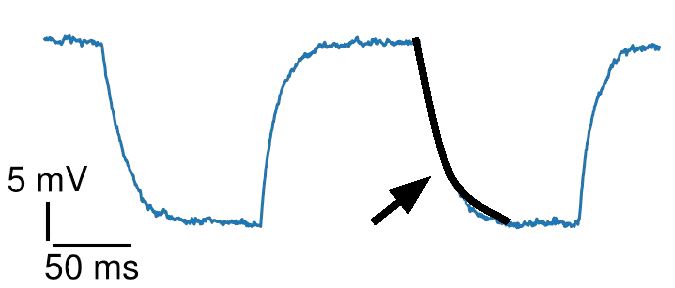
\includegraphics[width=\textwidth]{img/chapter4/neuron_TC.pdf}
  \subcaption{}
  \label{fig:neuron_TC}
  \end{subfigure}
  \begin{subfigure}[b]{.34\textwidth}
  \centering
  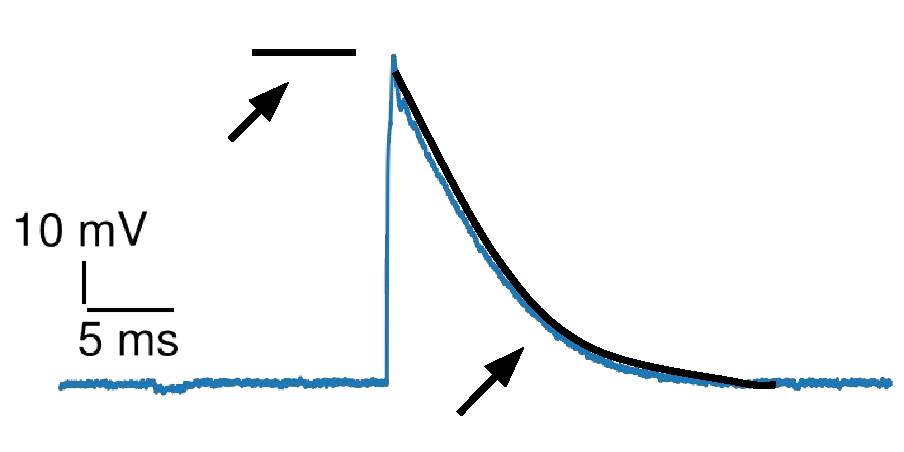
\includegraphics[width=\textwidth]{img/chapter4/ampa_tc.pdf}
  \subcaption{}
  \label{fig:ampa_tc}
  \end{subfigure}
  \caption[Automated measurement of neuron and synapse silicon circuit properties]{Automated measurement of neuron and synapse silicon circuit properties.
(\subref{fig:neuron_ref}):~Measurement of the refractory period of a neuron responding to constant input DC current.
(\subref{fig:neuron_TC}):~Measurement of neuron membrane time constant by fitting the relaxation part of the neuron response after the subthreshold DC current input.
(\subref{fig:ampa_tc}):~Measurement of amplitude (weight) and time constant of an excitatory synapse.}
  \label{fig:automated_acquisition}
\end{figure}

The synaptic weight and time constants of the synapse were estimated indirectly by analyzing the neuron membrane potential using a more elaborate protocol: we first set the neuron time constant to very short values to allow the neuron to follow its input currents faithfully%\dz{TBA: show how this is derived from the DPI equations}
; then, to generate excitatory or inhibitory post-synaptic potentials (EPSPs and IPSPs, respectively), we stimulated the neurons with $20$\,Hz spike trains and analyzed the pulse response decay in-between input spikes (see Fig.~\ref{fig:ampa_tc}). For inhibitory pulses, a constant DC current input was provided.

The weight values were estimated by measuring the PSP amplitude at the onset of the input spike, and the time constant was estimated by fitting the curve with a decaying exponential.

Here, it is essential to note that since the synapse circuit measurements are indirect, the absolute values of weights are not comparable across neurons, as the neuron circuits themselves overlay their variability profile. Those measurements allow, however, balancing EPSPs vs IPSPs within the same core as they interact within the same neuron circuits.

According to the measurements performed, the neuron time constant parameter has a CV of 18\%, and it's refractory period of 8\%.
Similarly, the CV of the synapse time constant ranges between 7\% and 10\% depending on its type (NMDA or AMPA) and the weight parameter from 14\% to 30\%.

\begin{figure}[h]
\centering
  \begin{subfigure}{.32\textwidth}
  \centering
    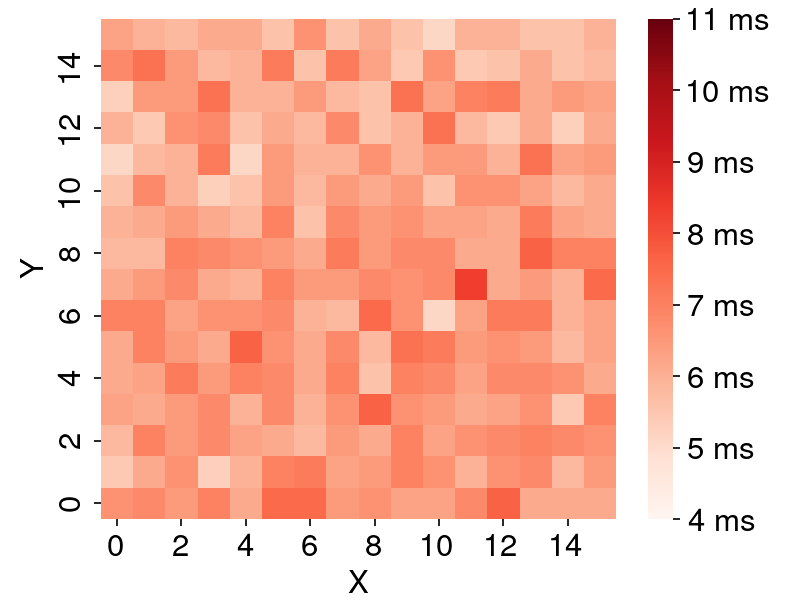
\includegraphics[width=\textwidth]{img/chapter4/rfr_spatial_distribution.png}
    \subcaption{}
    \label{fig:tau_ref_spatial_dist}
  \end{subfigure}
    \begin{subfigure}{.32\textwidth}
    \centering
    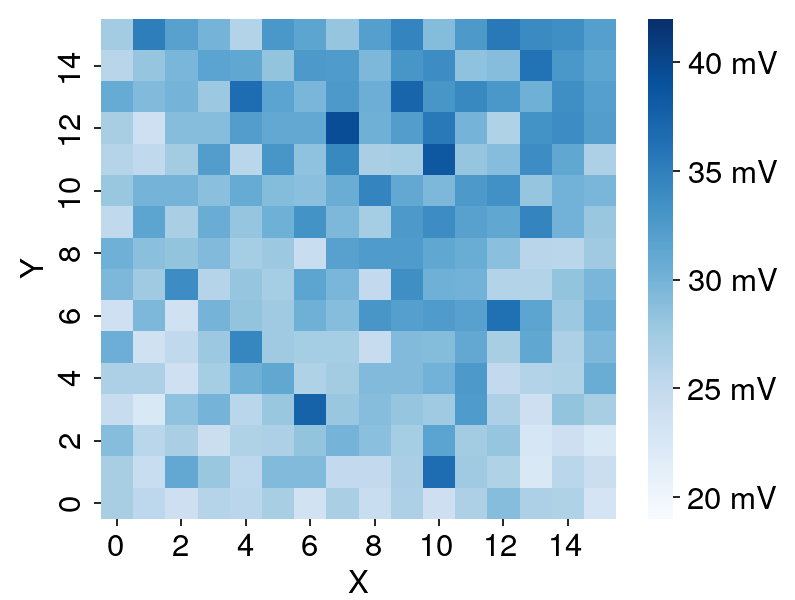
\includegraphics[width=\textwidth]{img/chapter4/wgt_spatial_distribution.png}
    \subcaption{}
    \label{fig:wgt_spatial_dist}
  \end{subfigure}
    \begin{subfigure}{.32\textwidth}
    \centering
    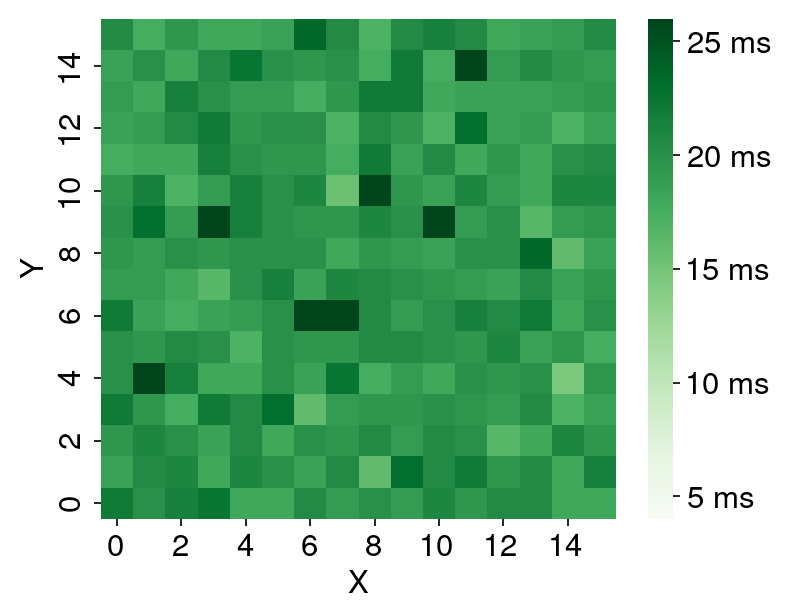
\includegraphics[width=\textwidth]{img/chapter4/tau1_spatial_distribution.png}
    \subcaption{}
    \label{fig:tau1_spatial_dist}
  \end{subfigure}
  \caption[Spatial distribution of mismatch profiles for the neuron and synapse parameters]{Spatial distribution of mismatch profiles for the neuron refractory period (\subref{fig:tau_ref_spatial_dist}), the synaptic weight (\subref{fig:wgt_spatial_dist}), and the neuron time constant (\subref{fig:tau1_spatial_dist}). The $X$ and $Y$ axes represent the neuron id across the layout of the measured core. The measurements were taken for the main fixed set of parameters used to obtain the results.}
  \label{fig:core_spatial_mismatch}
\end{figure}

Even though the variability of different parameters can exhibit different spatial distributions across the chip area, as evidenced by the patterns shown in Fig.~\ref{fig:core_spatial_mismatch}, these spatial distributions differ for each parameter and are generally uncorrelated between parameters.

%\dz{TBA: Show proof (correlograms)?}

As a consequence, the superposition of these effects results in a heterogeneous neuron firing behavior that has no particular correlation with the location of the neuron on the chip layout, or with the specific chip used.

\begin{figure}[h]
  \begin{subfigure}{.5\textwidth}
    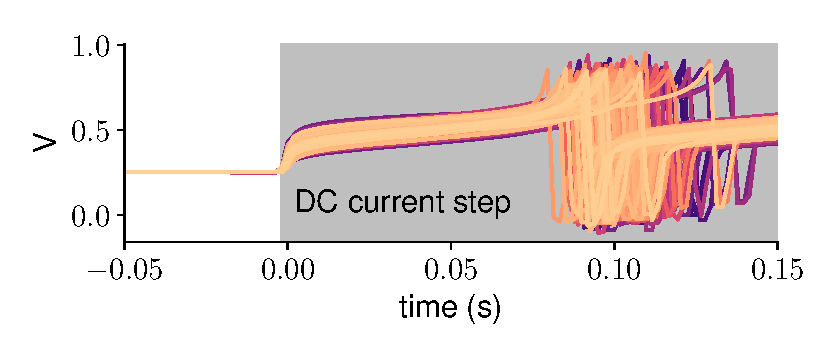
\includegraphics[width=\textwidth]{img/chapter4/ttfs_waveforms.pdf}
    \subcaption{}
    \label{fig:spike_wfs}
  \end{subfigure}
  \begin{subfigure}{.475\textwidth}
    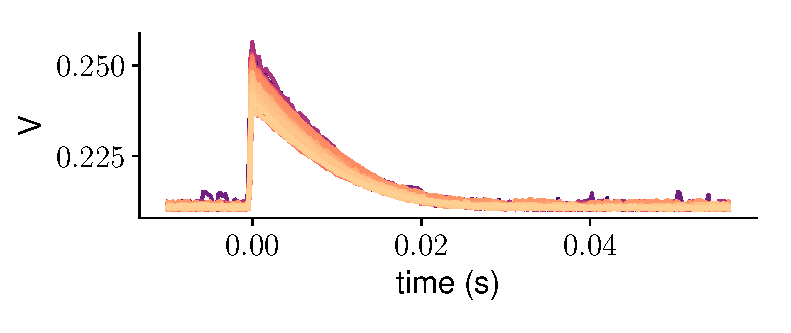
\includegraphics[width=\textwidth]{img/chapter4/epsp_c0c4.pdf}
    \subcaption{}
    \label{fig:epsp_wfs}
  \end{subfigure}\\
  \begin{subfigure}{.5\textwidth}
    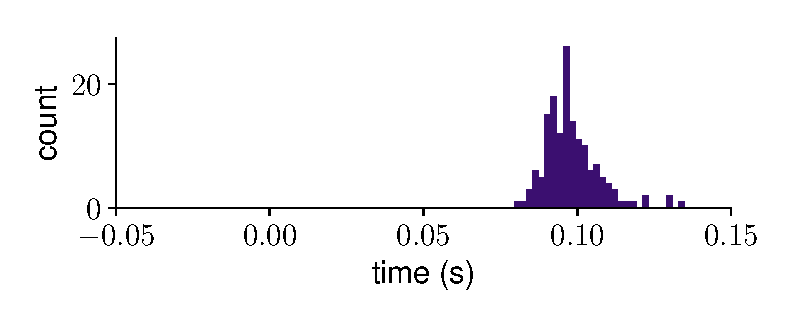
\includegraphics[width=\textwidth]{img/chapter4/ttfs_distribution.pdf}
    \subcaption{}
    \label{fig:ttfs}
  \end{subfigure}
  \begin{subfigure}{.475\textwidth}
    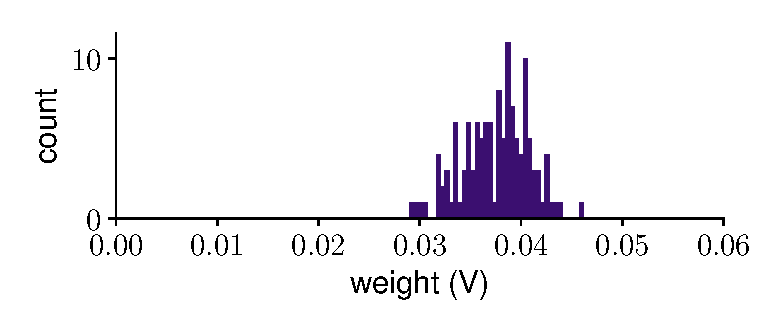
\includegraphics[width=\textwidth]{img/chapter4/epsp_amplitudes_distribution.pdf}
    \subcaption{}
    \label{fig:wfs_dist}
  \end{subfigure}
  \caption[Neuron and synapse variability.]{Neuron and synapse variability.
(\subref{fig:spike_wfs}) Aligned membrane voltage recordings of 256 neuron circuits of one DYNAP-SE core, sharing the same parameters,   in response to a common DC step input current.
Due to device mismatch, the time-to-first-spike of each neuron is distributed normally with CV=9\%; (\subref{fig:epsp_wfs}) Aligned impulse responses of 256 synapse circuits of the same core.
Due to device mismatch the height of the impulse response is distributed around a mean value that is proportional to the same synaptic weight parameter; (\subref{fig:ttfs}) and (\subref{fig:wfs_dist}) show the distributions of the measurements.
  The variation of responses is the cumulative result of individual properties distributions.}
  \label{fig:variability}
\end{figure}


Figure~\ref{fig:variability} shows measurements of such of heterogeneous neuron firing on the DYNAP-SE\@.
For example, when injecting the same input current to multiple instances of \ac{ADEXP-LIF} neurons of one core, the integration and spike generation circuits produce different delays in the time-to-first-spike (see Fig.~\ref{fig:spike_wfs}).
Similarly, when multiple synapses that share the same weight and time constant parameters are stimulated, the device mismatch in these circuits affects the shape of their response (see Fig.~\ref{fig:epsp_wfs}).
When measured across multiple instances of synapse and neuron circuits belonging to the same chip, the response properties of the neuromorphic circuits produce distributions which have typical coefficients of variation (CVs) ranging from 10\% to 20\% (e.g., see Fig.~\ref{fig:ttfs} and Fig.~\ref{fig:wfs_dist}).

%\dz{Requires a table of exact numbers}.

The next section explores how those distributions scale with parameter settings and how this tuning process can be optimized.


\subsection{Setting biases (at scale).}

On the DYNAP-SE1 chip, the parameters neuron and synapse circuits are controlled by bias currents set by 12\,bit temperature-compensated on-chip bias generators~\cite{Delbruck_etal10}.
All 25 available parameters (the main parameters indicated by red arrows in Figure~\ref{fig:DPI_neuron_and_synapse}) are globally shared within a core, and there are four independent bias generators per chip (one per core).

The generated bias current $I_{bias}$ is defined by a 3-bit \emph{coarse} and a 8-bit \emph{fine} values:

\begin{equation}
I_{bias} \approx \textrm{fine}\frac{I_{max}[\textrm{coarse}]}{2^8-1}
\label{eq:bias_current}
\end{equation}
 where


\begin{figure}[t!]
    \begin{subfigure}{.47\textwidth}
    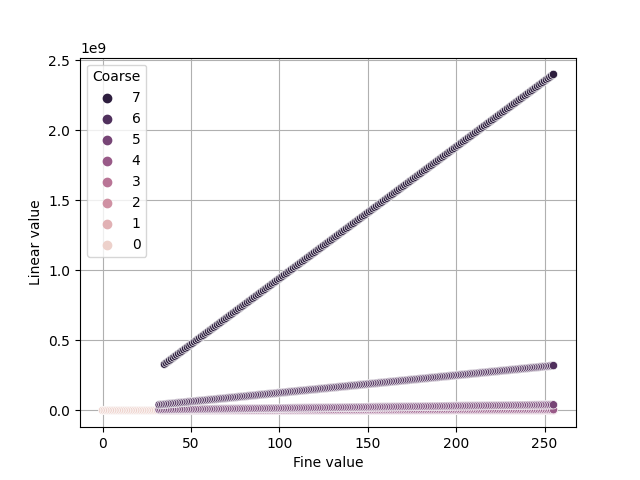
\includegraphics[width=\textwidth]{img/chapter4/linear_bias_map_full.png}
    \subcaption{}
    \label{fig:linear_bias_map_full}
  \end{subfigure}
  \begin{subfigure}{.47\textwidth}
    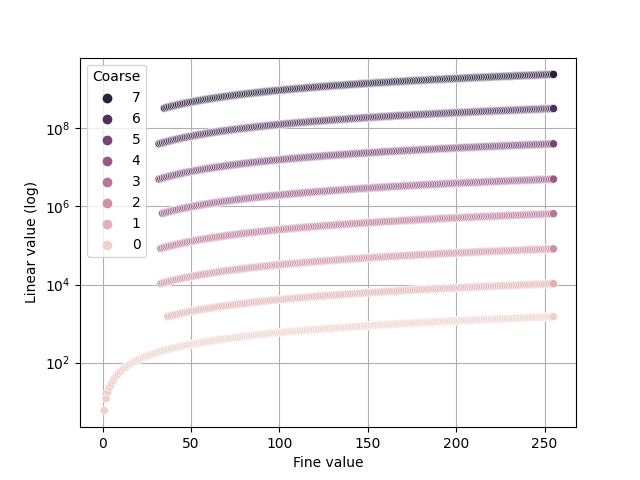
\includegraphics[width=\textwidth]{img/chapter4/linear_bias_map_log.png}
    \subcaption{}
    \label{fig:linear_bias_map_log}
  \end{subfigure}
  \caption[Linear bias value look-up table]{Linear bias value (proportional to the bias current) as a function of the fine and coarse values of the bias generator shown in linear (\subref{fig:linear_bias_map_full}) and logarithmic scale (\subref{fig:linear_bias_map_log}).} 
  \label{fig:linear_bias_map}
\end{figure}

\begin{figure}[b!]
\centering
  \begin{subfigure}{.47\textwidth}
    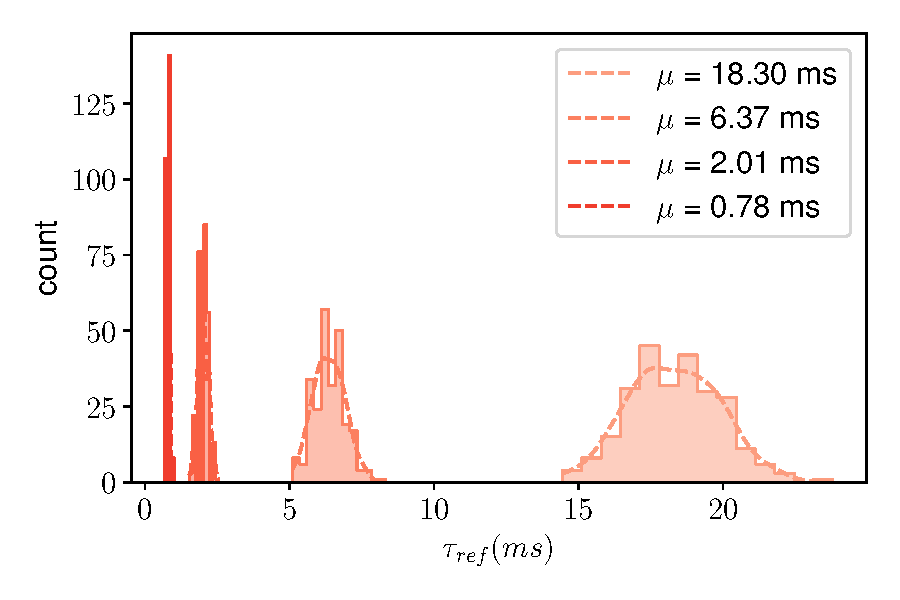
\includegraphics[width=\textwidth]{img/chapter4/scaling_tau_ref.pdf}
    \subcaption{}
    \label{fig:tau_ref_scaling}
  \end{subfigure}
  \centering
  \begin{subfigure}{.47\textwidth}
    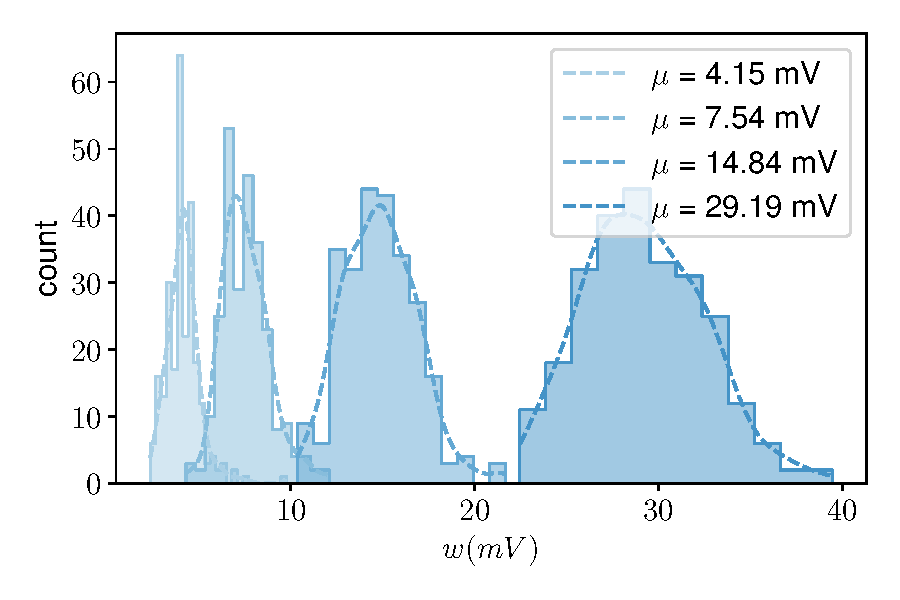
\includegraphics[width=\textwidth]{img/chapter4/scaling_nmda.pdf}
    \subcaption{}
    \label{fig:nmda_wgt_scaling}
  \end{subfigure}\\
  \centering
  \begin{subfigure}{.47\textwidth}
    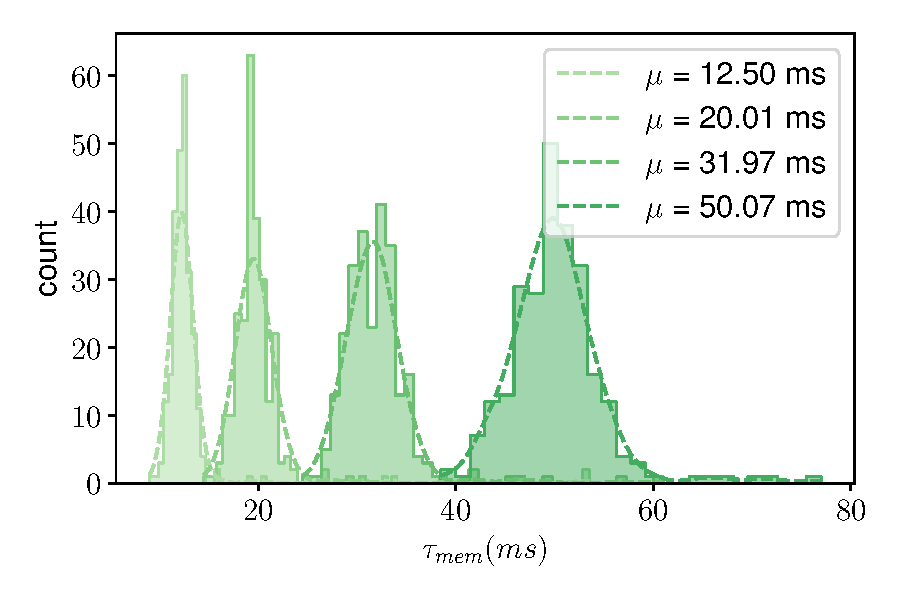
\includegraphics[width=\textwidth]{img/chapter4/scaling_tau_mem.pdf}
    \subcaption{}
    \label{fig:neuron_tau_scaling}
  \end{subfigure}
  \centering
  \begin{subfigure}{.47\textwidth}
    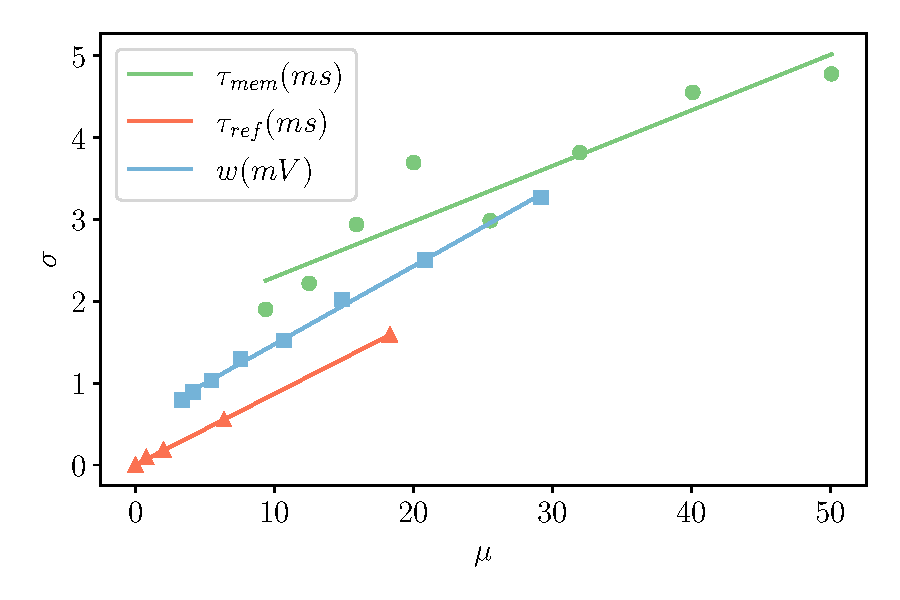
\includegraphics[width=\textwidth]{img/chapter4/scaling_all.pdf}
    \subcaption{}
    \label{fig:bias_CV_scaling}
  \end{subfigure}
  \caption[Variance behaviour across different properties of the DPI neuron circuit (parameter scaling)]{Variance behaviour across different properties of the DPI neuron circuit: (\subref{fig:tau_ref_scaling}) neuron refractory period, (\subref{fig:nmda_wgt_scaling}) synapse weight and (\subref{fig:neuron_tau_scaling}) neuron time constant measured across 256 neurons of the same core for 4 different bias values (shown in shades of the respective color).
  The plot in (\subref{fig:bias_CV_scaling}) shows how the variance changes with the mean, confirming that the CV remains approximately constant for all these parameters.}
  \label{fig:variance}
\end{figure}

 \begin{itemize}
     \item $I_{max} =[15,105,820,6.5 \cdot 10^3, 50 \cdot 10^3, 0.4 \cdot 10^6, 3.2 \cdot 10^6, 24 \cdot 10^6]$ pA
     \item fine $\in [0,255]$, coarse $\in [0,7]$
 \end{itemize}


Note that $I_{max}$ is an estimate and is subject to variability from chip to chip due to mismatch in bias generator circuits. Still, while the Python library \pyobject{samna}~\cite{Samna} used to work with the DYNAP-SE1 chip accepts the coarse and fine bias values, we can use a single continuous \emph{linear} bias parameter that is proportional to $I_{bias}$ and scales continuously between the minimum and maximum current values, to build mappings to physical circuit properties, making the transition to the next \emph{coarse} value when the maximum \emph{fine} value for the current \emph{coarse} value is reached. In Figure~\ref{fig:linear_bias_map_full}, the linear and the logarithmic scales for linear bias values show the graphical representation of such a non-overlapping map. Notable, the higher the $I_{bias}$ current, the lower the precision of it because of the \emph{fine} value discrete step multiplication by the coarse value.

\begin{figure}[t!]
  \centering
  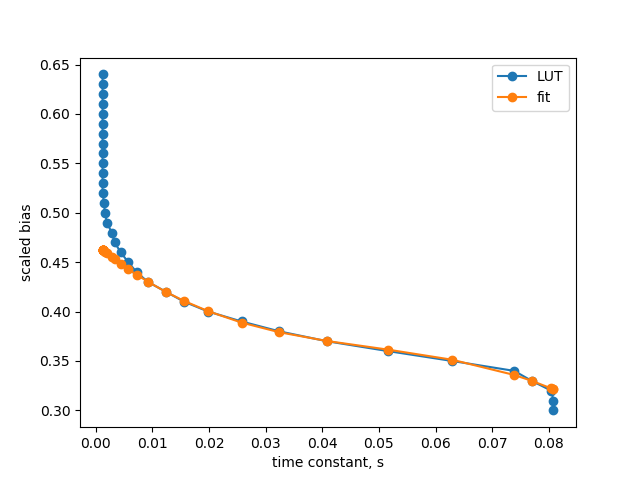
\includegraphics[width=0.8\textwidth]{img/chapter4/Bias_curve.png}
  \caption[Example of a LUT collected for a neuron's time constant]{A map (or a \ac{LUT}, in blue) of a normalized bias value of a neuron membrane leak bias to a mean value of the measured time constant (in seconds) set for the DYNAP-SE1 core. The measurement shows that only a short range of approximately 10\% of the bias values covers the entire range of usable parameter values. A polynomial fit for the usable parameter range is shown in orange, which allows setting interpolated bias values.
  Due to variability, for every core, this range would be shifted.}
  \label{fig:bias_curve_fit}
\end{figure}

Having the automated measurement tools and an understanding of the bias generator, we can start building the mapping between simulation and hardware mentioned in Section~\ref{subsec:triangle_of_relations}.
The final missing piece is the understanding of how the values scale with the bias value.
In Figure~\ref{fig:variance}, we show the detailed distributions of the same three parameters (neuron refractory period, neuron time constant and the AMPA weight) measured across 256 neurons of one core for 4 different values of the bias current for each property.

\begin{figure}[b!]
\centering
  \begin{subfigure}{.6\textwidth}
    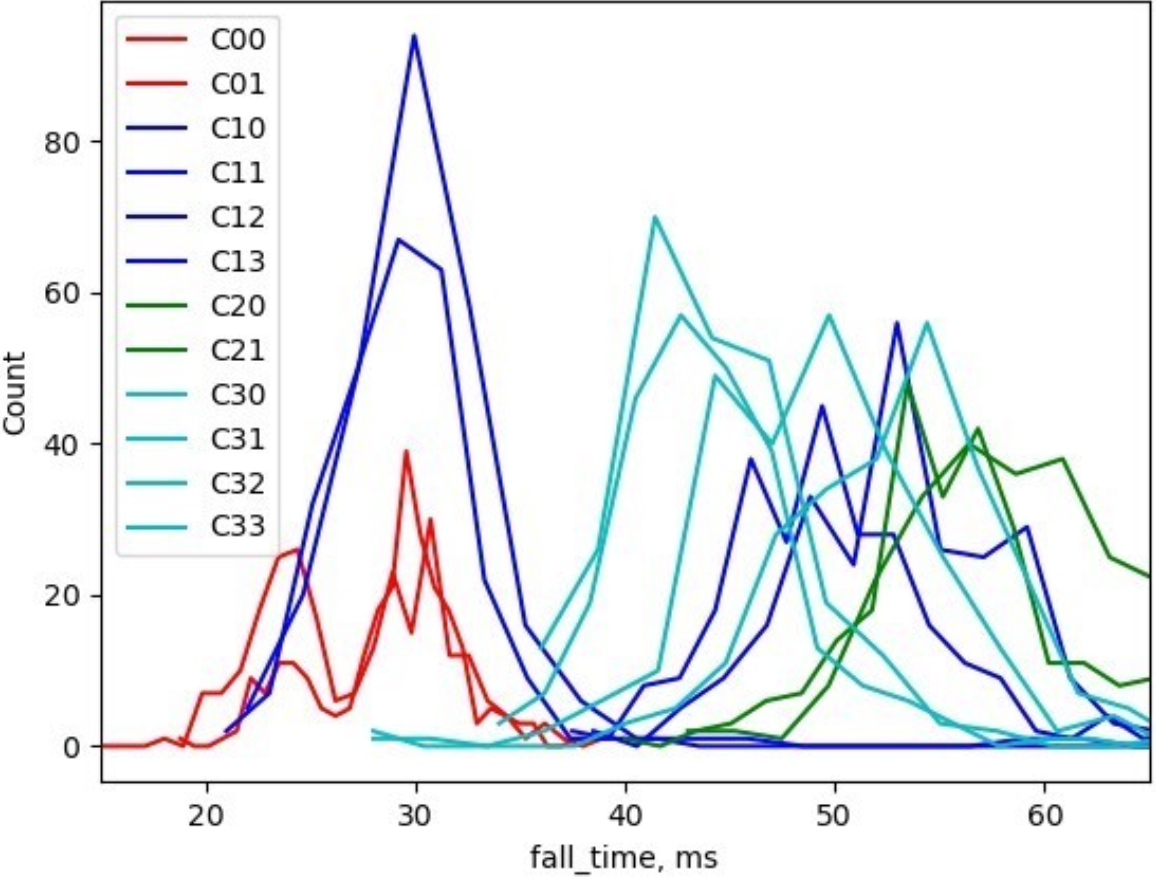
\includegraphics[width=\textwidth]{img/chapter2/cores_TCs_same_bias.png}
    \subcaption{}
    \label{fig:TCs_same_bias}
  \end{subfigure}\\
  \centering
  \begin{subfigure}{.65\textwidth}
    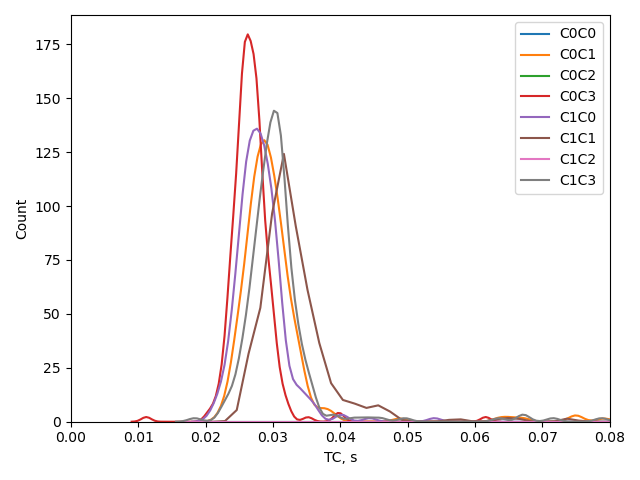
\includegraphics[width=\textwidth]{img/chapter2/taus_tuned_to_30ms_dist_new.png}
    \subcaption{}
    \label{fig:TCs_same_mean}
  \end{subfigure}
  \caption[The result of using the tuning framework to align the time constants across multiple cores of the DYNAP-SE1 chip.]{Tuning the neuron time constant across multiple DYNAP-SE1 cores. Both plots show histograms of distributions of time constants, with one line corresponding to one core of 256 neurons. (\subref{fig:TCs_same_bias}) Result of copying the same bias values across multiple cores. The distributions are located far apart as a result of mismatch both in neuron circuits and in bias generator blocks. Different colours correspond to different chips. (\subref{fig:TCs_same_mean}) Neuron time constant distributions set to a 30ms mean using the LUTs of the \pyobject{BiasTuner} framework. While still not perfectly aligned, the distributions are brought much closer together.}
  \label{fig:TC_tuning}
\end{figure}

As shown in Fig.~\ref{fig:bias_CV_scaling}, the CV of such distributions tends to stay constant across different bias current settings.
This allows to determine exact mismatch measures for individual properties across every core. Specifically, we confirm that the scaling of the properties is uniform, i.e. the neuron with a low time constant compared to the rest of the neurons of the core at a lower bias value would stay at the same part of the distribution for the higher bias value.


Therefore, a tuning strategy optimizing the amount of necessary measurements taken can be proposed. To create a mapping between the bias value and the parameter, a neuron that is close to the \emph{mean} of the parameter distribution can be picked. After the calibration LUT (look-up table) is collected, it can be interpolated within the usable parameter range (see the example for the neuron time constant in Figure~\ref{fig:bias_curve_fit}). Essentially, we pick a single neuron to represent the state of the core for a specific parameter. Note that the range where the parameter takes biologically plausible values is, in fact, narrow (10-15\%) compared to the full possible bias range. This range could be fitted well enough with a polynomial function to interpolate between the measured data points. 

The bias generators, however, are also subject to variability, which explains why the same bias values cannot be just copied between different chip cores. Specifically, Figure~\ref{fig:TCs_same_bias} shows the case when the same bias parameter is copied between multiple cores of multiple dynapse chips. The variability of bias generators defines the locations of means of neuron time constant distributions, while the variability of neuron circuits causes the width of each distribution. On Panel~\ref{fig:TCs_same_mean} these distributions are moved together using the calibration procedure shown in Figure~\ref{fig:bias_curve_fit}, using the interpolated LUTs to set the 30ms means. As a result, the behaviour of the neurons across cores is unified.
\\


\newpage
\section{Averaging across space and time}
\label{sec:averaging}

Spiking neural electronic systems made of high-precision components or ideal neurons in computer simulations represent signals with high fidelity.
In analog circuits, very high levels of precision for representing signals can be achieved only at great costs.
Alternatively, a practical solution, extensively exploited also in the brain, is to relax the high precision constraint for single computational units, the neuron, and to distribute computation in space and time.
Feeding signals to populations composed of heterogeneous units with uncorrelated mismatch in their properties, as in Fig.~\ref{fig:ff_curves}, naturally reduces the effect of noise and variability in the single units.
Averaging signals over time filters out irregularities in the spike sequences generated by both the input sensors and by the neural processing parts of the system.

Figure~\ref{fig:ff_curves} shows the combined effect of both synapse and neuron variability: the plot shows the average firing rate of 16 neurons belonging to the same core, and sharing the same parameter settings.
Each neuron is stimulated via its own excitatory synapse, driven by the same set of input spike sequences of increasing frequency. Although the variability of both synapse and neuron parameters produces response profiles with large differences, the ensemble average response follows the desired profile with good linearity.

\begin{figure}[h!]
\centering
    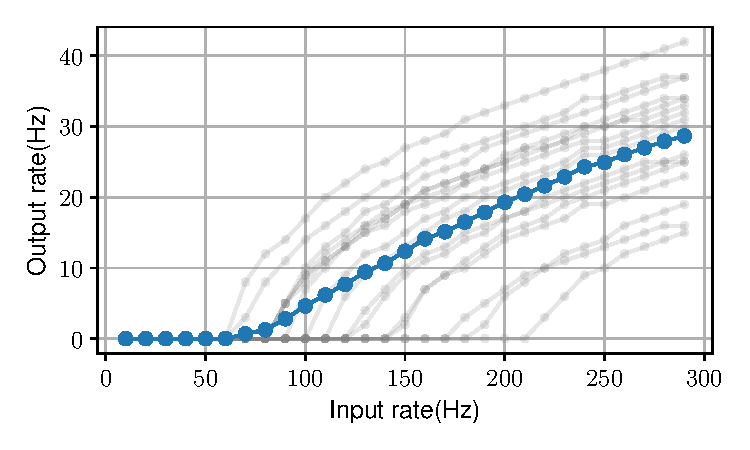
\includegraphics[width=.7\textwidth]{img/chapter4/ff_curves_all.pdf}
  \caption[Variability in transfer functions of 16 silicon neurons.]{Firing rate of 16 silicon neurons belonging to the same core, thus sharing the same parameter settings. All neurons are driven by the same series of regular spike trains with constant rates over one second and step increments of 10\,Hz.}
\label{fig:ff_curves}
\end{figure}

\begin{figure}[h!]
    \centering
    \begin{subfigure}[b]{0.5\textwidth}
        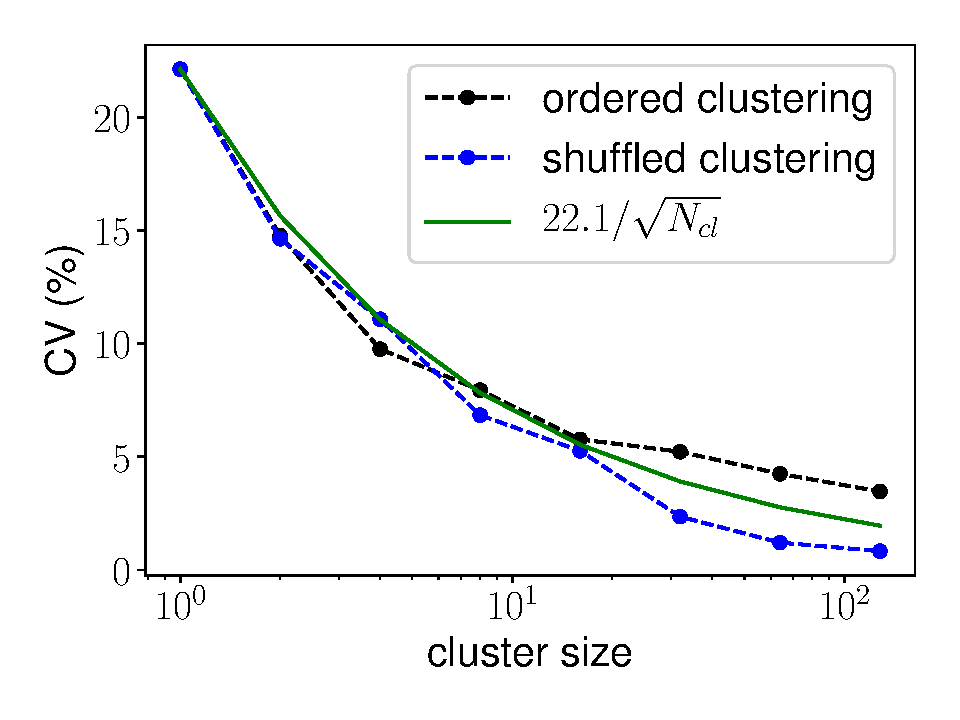
\includegraphics[width=\textwidth]{img/chapter4/CV_clustering_at_50Hz.pdf}
        \caption{}
        \label{fig:variance_vs_cluster_size_a}
    \end{subfigure}\\
        \centering
    \begin{subfigure}[b]{0.7\textwidth}  
        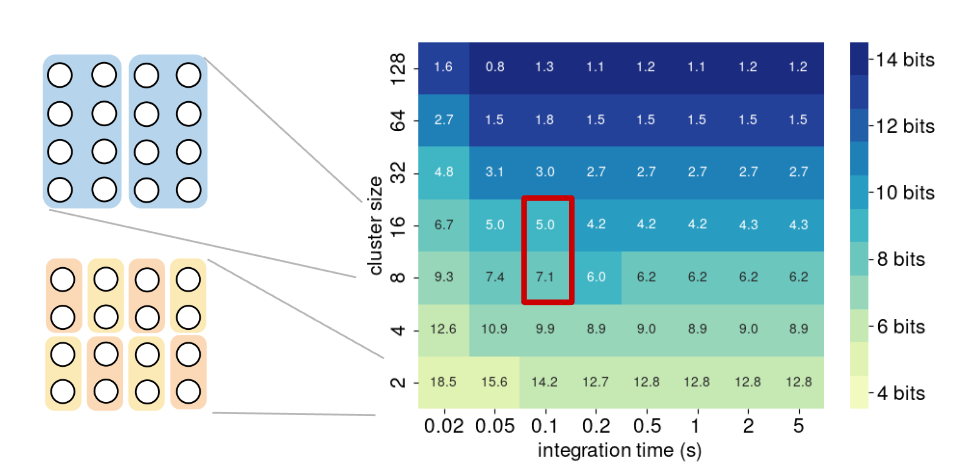
\includegraphics[width=\textwidth]{img/chapter2/Cluster_size_tradeoff.png}
        \caption{}
        \label{fig:variance_vs_cluster_size_b}
    \end{subfigure}
    \caption[Variance of the mean firing rates of clusters of neurons decreases with cluster size]{Variance of the mean firing rates of clusters of neurons decreases with cluster size.
(a): recordings from 256 neurons of the chip with different cluster arrangement (black line for sequential and blue line for randomly shuffled clustering).
All 256 neurons were used at all times, meaning the largest CV is for 256 clusters of size 1, and the lowest is for 2 clusters of size 128.
The green line is a $1/\sqrt{N_{cl}}$ fit normalized to the first value.
The integration time is 1 sec.
(b) Dependence of cluster rate CV (shown in each color coded square) on cluster size (y-axis) and spike integration time (x-axis).
The equivalent bit precision for each CV value is color coded.
Each CV value shown is a mean across 10 random splits (shuffles) into clusters.
Darker color stands for higher precision of encoding.}
    \label{fig:variance_vs_cluster_size}
\end{figure}


The first strategy, of \emph{space averaging encoding}, can be implemented, for example, by feeding the output spike train of one unit to multiple neurons in a cluster.
%(see Fig.~\ref{fig:rate-population}).
We tested this strategy by carrying out an experiment in which a node producing a regular spike train of $200$\,Hz drives a population of 256 neurons, in one DYNAP-SE core, in a way to produce an average output rate of $50$\,Hz.
We computed their individual output firing rates during one second of recording and used its distribution across the cluster to compute the rate CV of different size clusters, ranging from two clusters of 128 neurons to 4 clusters of 64 neurons each, to 8 of 32 neurons, and so on, up to 256 clusters each made of one neuron.
For each combination, the CV of the rate is computed from the mean and variance of the firing rate distribution across clusters, grouping neurons selected within the same single core. 
To measure average values of the CV, we computed the mean CV over $10$ reconstructions of the same configuration with shuffled (regrouped) neurons across clusters.
Figure~\ref{fig:variance_vs_cluster_size_a} shows the firing rate CV computed in this way, as a function of cluster size.
Our data are consistent with the averaging theory, which states that the standard deviation and the coefficient of variation of a distribution is proportional to the $\sqrt{N_{cl}}$, where $N_{cl}$ is the cluster size (see Fig.~\ref{fig:variance_vs_cluster_size_a}).
Thus, the balance between employed resources and acceptable cancellation of mismatch, i.e., firing rate CV reduction, results from a trade-off that scales with $\sqrt{N_{cl}}$.


In the second \emph{time averaging encoding} strategy, the integration time window is a relevant parameter.
Unlike neurons simulated with digital hardware, but very much like biological ones, mixed signal analog/digital silicon neurons produce irregular spike trains even if stimulated with constant inputs, and exhibit heterogeneity in their firing rates across multiple trials even if the input stimulus is always the same.
If we fix an integration bin size, within the same bin, fast firing neurons provide more information than slow ones.
In Fig.~\ref{fig:variance_vs_cluster_size_b}, we estimate the CV for increasing bin sizes, ranging from 20\,ms up to 5\,seconds, calculated for each choice of cluster size.
The trade-off between readout time and amount of resources is now evident: precise rate encoding requires large clusters.
For example, in this experiment an equivalent bit precision of 14\,bits is achieved only by using clusters that comprise 128 neurons.
However, by combining longer integration times (e.g., 100\,ms--200\,ms) with cluster sizes of 8 or 16 neurons it is possible to achieve equivalent bit precision of 8\,bits, which appears to be adequate for many artificial intelligence and neural processing tasks~\cite{Pfeil_etal13,Stromatias_etal15a,Baldassi_etal16}.

An advantage of this approach is that the chip designer does not have to make critical decisions (such as choosing the number of bits to use in a digital bus) at chip design time. The size of the cluster and the integration time can be flexibly changed and even adapted dynamically at run time. 

%\subsection{Population coding as a method to combine rate and space coding}

%\dz{To Be Changed: Move the population coding introduction to here from Chapter 3? Because technically for population coding we do not need to connect any neurons yet.}

%In the array of $N$ input channels, the firing rates would be defined as set the input neuron rates

%\begin{equation}
%    r_i = r_{max} e^{-\frac{1}{2} \frac{(i-\mu-N/2)/N}{\sigma}^2}
%    \label{eq:popcode2rates}
%\end{equation}


\section{Discussion: temperature-induced variability}

In this chapter, we have introduced the systematic device characterization and tuning method. It allowed us to observe the true mismatch profile of multiple DYNAP-SE1 cores in a relatively short amount of time, which was not possible before. This, in fact, allowed to schedule the automated measurement at the different times of day, returning an interesting results shown in Figure~\ref{fig:TC_temperature_variability}.

It shows temperature-induced variability for two measurements taken during the summer day and two at night (of the same day). While the exact temperature delta was not recorded, it should not have changed for more than 10-15C. On the one hand, this measurement aswers how bad the temperature effect really is on the neuron circuits. The answer is that the entire distribution of the time constants can move for almost 1 sigma. On the other hand, this means that our LUTs collected for systematic parameter setting are not that precise: the observed thermal shift would easily convert the requested 30ms time constant into a 25ms one. While this might not look too critical, this is another factor that can through a spiking system out of balance.

\begin{figure}[h]
\centering
    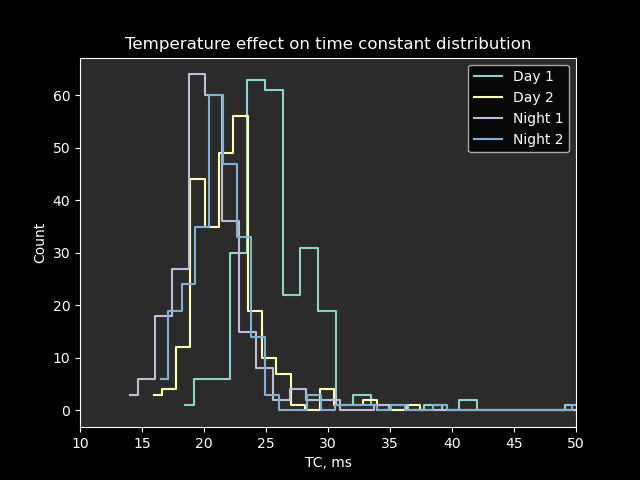
\includegraphics[width=.7\textwidth]{img/chapter2/time_constant_distribution_vs_temperature.png}
  \caption[Temperature dependence illustration]{Distribution of neuron time constants of a single core of 256 neurons of the DYNAP-SE1 chip evolving across multiple days. The distributions might shift by almost one $\sigma$, which is an effect of temperature-induced parameter variability.}
\label{fig:TC_temperature_variability}
\end{figure}


\newpage

\chapter{Connecting neurons. Dynamics in static networks.}
\label{ch:static_networks}

In this chapter, having equipped the tools and configuration guidelines for the neural assemblies, we begin connecting the neurons of the \ac{DYNAP}-SE1 together into static (fixed-connectivity) circuits of coupled excitatory and inhibitory populations. 

\section{Neural coding strategies}

%\dz{TBA: Equation for Gaussian input. An equation for population code value extraction.}

\emph{Encoding} signals in a robust and reliable manner is a fundamental step for processing and computing.
In the nervous system, this is done seamlessly at the site of sensory input and further elaborated at relay stations along the path to the central nervous system via populations of neurons.
%To \emph{encode} signals using single clusters of neurons that can ensure high accuracy is important.
However, to carry out robust neural computation, it is also important to choose the proper way to \emph{represent} signals.
A common strategy adopted by the nervous system is to use distributed representations~\cite{Dayan_Abbott01}, such as population codes~\cite{Averbeck_etal06}.
% Distributed representations are widely used in the brain.
Population codes are used across the nervous system to represent many types of signals, such as visual~\cite{Franke_etal16} or auditory cues and their spatial localization~\cite{Fitzpatrick_etal97}.
Population codes, and more generally distributed representations, are tolerant to damage, noise, and in the case of neuromorphic implementations, to device mismatch.
Indeed, heterogeneity and neuronal diversity in population coding can greatly enhance the network's information capacity~\cite{Shamir_Sompolinsky06}.

A basic distributed representation can be implemented by using populations of neurons subdivided into independent clusters that represent the value of their input signal.
%, the neurons in the cluster average out the noise due to devise mismatch.
To assess the benefits of this representation in mixed-signal neuromorphic systems, we performed an experiment in which we encoded the activity of input nodes with populations of silicon neurons arranged as uncoupled clusters (see Fig.~\ref{fig:decoupled_sketch}). Each cluster comprises a set of neurons that are not interconnected, but that receive the same spike train from the cluster's input node.
Figure~\ref{fig:bump_decoupled} shows the response of the cluster neurons to a bump signal spatially distributed across the input nodes.
Note that, although the input nodes have a one-to-one non-overlapping connectivity to the neuron clusters, we activate all of them in parallel with a spatially distributed profile  to emulate a distributed representation also at the input level.

\begin{figure}[h!]
\centering
\begin{subfigure}{0.45\textwidth}
\centering
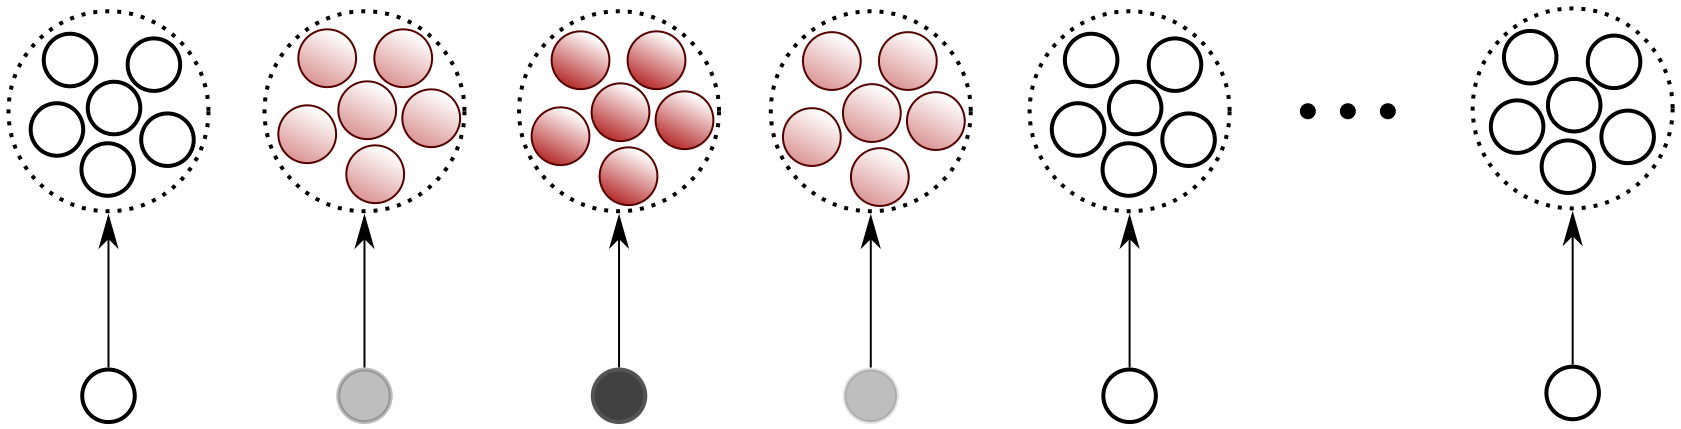
\includegraphics[width=0.85\linewidth]{img/chapter4/decoupled_sketch.png}
\caption{}
\label{fig:decoupled_sketch}
\end{subfigure}
\begin{subfigure}{.5\textwidth}
\centering
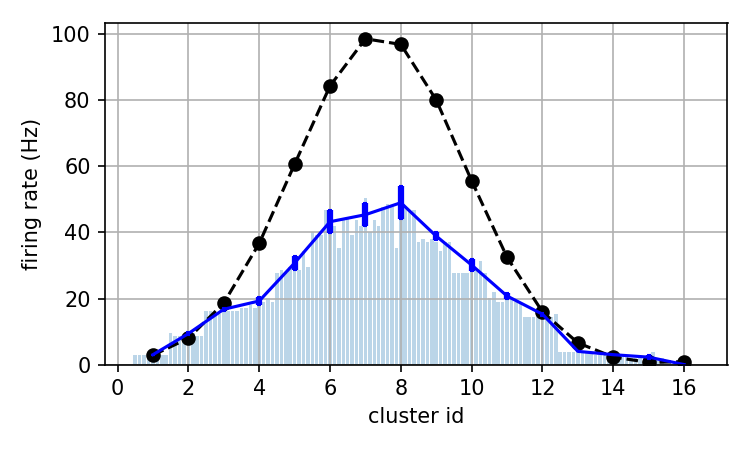
\includegraphics[width=\textwidth]{img/chapter4/clustered_inh_WTA_bump_sharpening_base.png}
\caption{}
\label{fig:bump_decoupled}
\end{subfigure}
\caption[Population code with decoupled clusters]{Multiple decoupled clusters of neurons representing a distributed population code.
(\subref{fig:decoupled_sketch}) Network diagram.
Sixteen independent clusters of 8 silicon neurons each receive spikes from individual input nodes whose firing rates change smoothly with spatial position (shades of gray). Each neuron in a cluster receives the same spike sequence and contributes to the cluster's average firing rate.
(\subref{fig:bump_decoupled}) Bump-shaped mean firing rates of the input nodes (black dots) and average output population activity (dark blue).
Error bars indicate the standard deviation within each cluster. The light blue bars represent the firing rate of individual neurons.}
\label{fig:population_coding_decoupled}
\end{figure}
%The neurons are driven with strong synaptic inputs, but have a large refractory period that forces them to saturate at relatively low firing rates. So the average output activity of these neurons can faithfully represent the input signals for small inputs, but distorts the input for higher input rates. 
Given their shared input and the strong synaptic weight values used, the neurons in each cluster would tend to produce strongly correlated spike trains if they were homogeneous. In our case, however, the heterogeneity of the silicon neuron circuits is beneficial in reducing the effects of strong input with temporal correlations. This has been shown to be effective in improving encoding accuracy~\cite{Ecker_etal11}.
Forcing the neurons to saturate at relatively low firing rates can be beneficial for reducing the overall system power consumption. However, it limits the output dynamic range of the neurons, and hinders their ability to faithfully encode inputs that have wide dynamic range.
This limited dynamic range problem is faced also by biological neurons: real neurons typically have low firing rates and a small dynamic range, compared to the signals they must represent, especially in the early sensory stages.
Using populations of heterogeneous neurons to average out the effects of variability can solve this limited dynamic range problem: as postulated in~\cite{Adam_etal20}, populations of $N$ integrate and fire neurons can faithfully encode band-limited signals that have $N$ times the bandwidth of individual neurons.
So resorting to the use of populations of neurons for representing signals while reducing the effect of variability has the added benefit of allowing the system to represent signals with high dynamic ranges that exceed the range of individual neurons.
Furthermore, an important requirement of this theory is that neurons do not start from identical initial conditions~\cite{Adam_etal20}. So using populations of \emph{heterogeneous} neurons, such as those implemented with analog circuits and/or with memristive devices, naturally satisfies the requirements of the theory.
To validate this theory with our neuromorphic circuits, we carried out an experiment in which we stimulated with a single Poisson input spike train a population of silicon neurons in a cluster of 16 units. The input node was configured to spike with an average firing rate of 100\,Hz, while all neurons in the cluster produced firing rates with a maximum value of about 40\,Hz. 
Figure~\ref{fig:single_cluster_variability} presents the experimental measurements.
As shown in panels~\ref{fig:single_cluster_inp_sketch}--\subref{fig:single_cluster_feedforward_ff_curves}, although individual neurons in the cluster cannot reproduce the fine details of the high dynamic range input signal, the population average (represented by the red line in the raster plots) can follow the input reliably.
There is strong evidence that real neural systems also use this strategy, for example to encode signals in the vestibular system~\cite{Sadeghi_etal07}.


%\dz{Move the following to discussion?}
Also in this case, in addition to averaging and reducing the effect of variability, resorting to using populations of neurons produced extra important advantages for encoding high bandwidth signals with low-bandwidth (and low power) silicon neurons. Moreover, although we restricted the analysis of the networks using mean firing rates without studying the effects of precise spike-timing, the same networks could encode signals exploiting the dynamics and the timing of input/output signals, for example using rank-roder neural codes~\cite{Furber_etal07}.


\section{Balancing excitation and inhibition}

In addition to choosing the right representation, computation heavily relies on using \emph{gain} in the processing pathway.
One way to implement and modulate gain in networks of neurons is to change the strength of the synaptic weights from layer to layer.
However, this process, typically achieved via synaptic plasticity, can be very slow and does not support modes of operation that require fast gain changes to carry out the desired computations.
Alternatively, a strategy commonly found in the nervous system that overcomes this problem is the use of recurrence, with both positive and negative feedback.
By adding recurrent excitation to the population of neurons, it is possible to control and modulate the gain of the network quickly, following the fast changes in the activity of neurons rather than the slow changes in synaptic efficacy of relevant synapses.
Indeed, as gain modulation is directly affected by the network activity, it can happen at much higher speeds than those dictated by plasticity mechanisms.


To demonstrate how this strategy is effective also for recurrent networks of silicon neurons, we added self-excitation to the cluster of 16 neurons of Fig.~\ref{fig:single_cluster_variability} (see Fig~\ref{fig:single_cluster_recurrent_sketch}).
This has the effect of increasing the gain of the network, driving the response of the network to much higher firing rates compared to the 40\,Hz baseline of panel~\ref{fig:single_cluster_feedforward_raster} (see red data in Fig.~\ref{fig:single_cluster_recurrent_raster}), while still being sensitive to the changes in the input signal, as evidenced by the linear input-output relationship measured in Fig~\ref{fig:single_cluster_recurrent_ff_curves}.
However, as this gain modulation is obtained via positive feedback, it can be difficult to control.
For example, in this case and with the parameter settings chosen, the network maintains its activity in a high persistent state even after the input has been removed.

\begin{figure}[h!]
  \centering
  \begin{subfigure}{.1\textwidth}
  \centering
  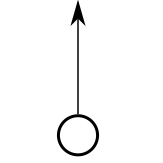
\includegraphics[width=.6\textwidth]{img/chapter4/Input_only.png}
  \caption{}
  \label{fig:single_cluster_inp_sketch}
  \end{subfigure}
  \hfill
  \begin{subfigure}{.5\textwidth}
    \centering
    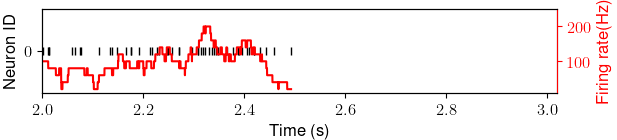
\includegraphics[width=\textwidth]{img/chapter4/raster_inp.png}
    \caption{}
    \label{fig:single_cluster_input_raster}
  \end{subfigure}
  \hfill
  \begin{subfigure}{.3\textwidth}
  \parbox{\textwidth}{}  
  \end{subfigure}
  \\ 
  \begin{subfigure}{.1\textwidth}
    \centering
    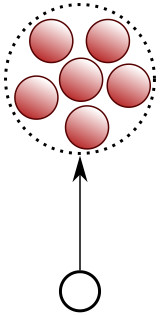
\includegraphics[width=.6\textwidth]{img/chapter4/FF.png}
    \caption{}
    \label{fig:single_cluster_feedforward_sketch}
  \end{subfigure}
    \hfill
  \begin{subfigure}{.5\textwidth}
    \centering
    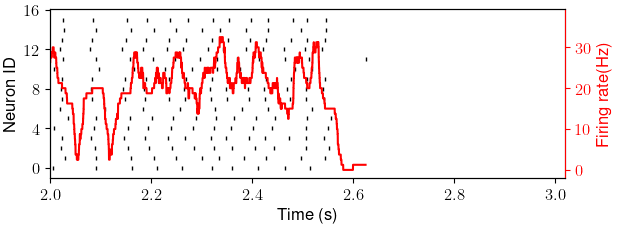
\includegraphics[width=\textwidth]{img/chapter4/raster_ff.png}
    \caption{}
    \label{fig:single_cluster_feedforward_raster}
  \end{subfigure}
    \hfill
  \begin{subfigure}{.3\textwidth}
    \centering
    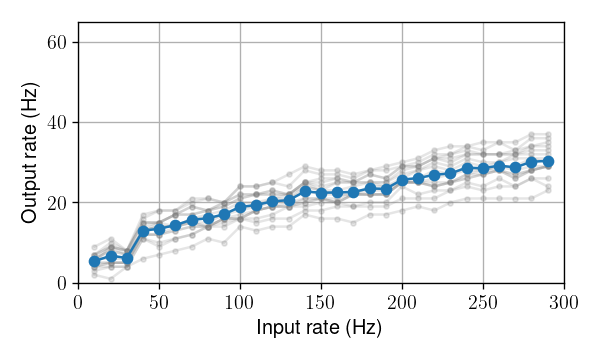
\includegraphics[width=\textwidth]{img/chapter4/FF_FF_curves.png}
    \caption{}
    \label{fig:single_cluster_feedforward_ff_curves}
  \end{subfigure}
  \\
  \begin{subfigure}{.1\textwidth}
    \centering
    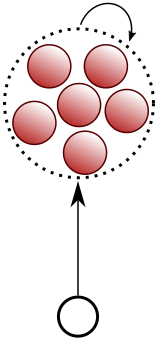
\includegraphics[width=.6\textwidth]{img/chapter4/FF_Rec.png}
    \caption{}
    \label{fig:single_cluster_recurrent_sketch}
  \end{subfigure}
    \hfill
  \begin{subfigure}{.5\textwidth}
    \centering
    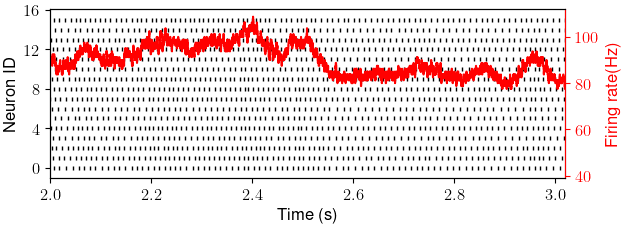
\includegraphics[width=\textwidth]{img/chapter4/raster_rec.png}
    \caption{}
    \label{fig:single_cluster_recurrent_raster}
  \end{subfigure}
      \hfill
  \begin{subfigure}{.3\textwidth}
    \centering
    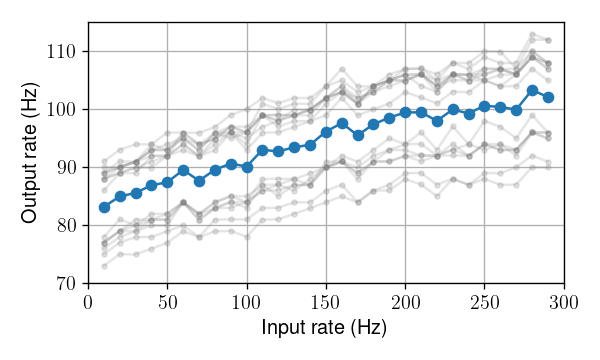
\includegraphics[width=\textwidth]{img/chapter4/EE_FF_curves.png}
    \caption{}
    \label{fig:single_cluster_recurrent_ff_curves}
  \end{subfigure}
  \\
  \begin{subfigure}{.1\textwidth}
    \centering
    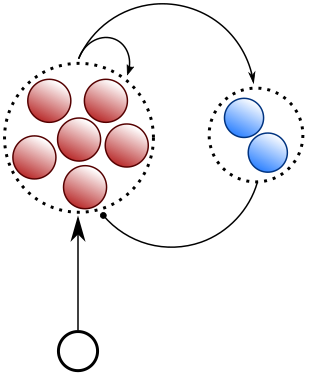
\includegraphics[width=.8\textwidth]{img/chapter4/EI_sketch.png}
    \caption{}
    \label{fig:single_cluster_feedback_sketch}
  \end{subfigure}
    \hfill
  \begin{subfigure}{.5\textwidth}
    \centering
    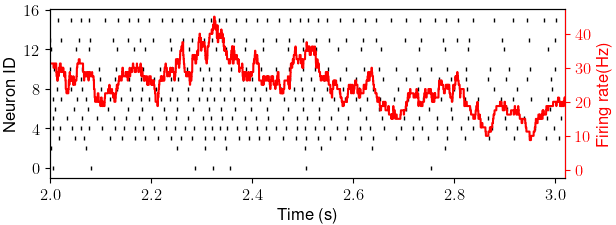
\includegraphics[width=\textwidth]{img/chapter4/raster_fb.png}
    \caption{}
    \label{fig:single_cluster_feedback_raster}
  \end{subfigure}
        \hfill
  \begin{subfigure}{.3\textwidth}
    \centering
    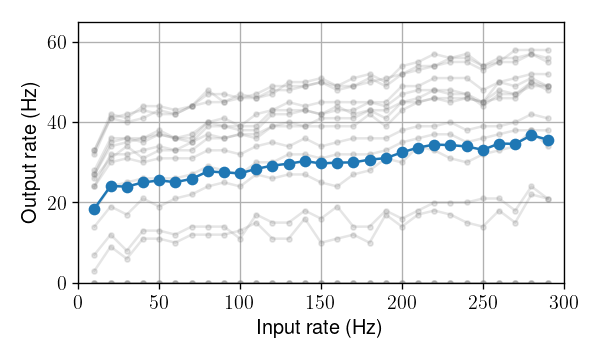
\includegraphics[width=\textwidth]{img/chapter4/EI_FF_curves.png}
      \caption{}
      \label{fig:single_cluster_feedback_ff_curves}
  \end{subfigure}
  \caption[EI coupling of a single cluster of neurons. Spiking activity decorrelation.]{Spiking response of a cluster of 16 neurons to the same Poisson input spike train (panel~\subref{fig:single_cluster_input_raster}) in 3 different connectivity configurations: pure feedforward (\subref{fig:single_cluster_feedforward_sketch}), with recurrent excitation (\subref{fig:single_cluster_recurrent_sketch}), with additional inhibitory feedback (\subref{fig:single_cluster_feedback_sketch}).
Panels on the right (\subref{fig:single_cluster_feedforward_ff_curves},\subref{fig:single_cluster_recurrent_ff_curves},\subref{fig:single_cluster_feedback_ff_curves}) show the response firing rates of individual neurons (gray traces) and the mean cluster firing rate (blue line) when feeding them with a regular spike train at different firing frequencies.
  The input spike train (\subref{fig:single_cluster_input_raster}) is fed to the cluster for each trial and the response rasters (\subref{fig:single_cluster_feedforward_raster},\subref{fig:single_cluster_recurrent_raster},\subref{fig:single_cluster_feedback_raster}) show the spiking response both during the input and after the input ends.
The mean firing rate of the cluster is shown in red.}
  \label{fig:single_cluster_variability}
\end{figure}


This can be a desirable effect for developing \emph{attractor networks}~\cite{Amit_etal85,Amit92}, but it can also be an undesired effect in other cases.
The brain-inspired strategy that can be used to keep this effect under control is to add a negative feedback loop in parallel with the positive feedback one.
This is achieved by projecting the activity of the excitatory neurons to a population of inhibitory neurons that, in turn, inhibits back the excitatory population (see Fig.~\ref{fig:single_cluster_feedback_sketch}, \subref{fig:single_cluster_feedback_raster}).


In the configuration of Fig.~\ref{fig:single_cluster_variability}, a single common Poisson source of spikes (with ISI $CV=1$) was used to stimulate all neurons in the cluster.
This led to correlated firing in the cluster, especially in the presence of recurrent excitation: the average ISI $CV$ of the population spike trains in Fig.~\ref{fig:single_cluster_recurrent_raster} decreased to 0.1. This impairs energy efficiency and is detrimental for signal encoding~\cite{Shadlen_Newsome98,Shamir_Sompolinsky06}.
Recurrent inhibition in architectures with excitatory and inhibitory synapses can help to decorrelate firing activity and significantly enhance coding efficiency~\cite{Tetzlaff_etal12,Zeldenrust_etal21,Koren_Panzeri22}.
This is also true for our silicon neuron network of Fig.~\ref{fig:single_cluster_feedback_sketch}. The recurrent inhibitory feedback leads to an excitatory/inhibitory balance that has the effect of producing sparse and decorrelated activity: the average ISI $CV$ of the data in Fig.~\ref{fig:single_cluster_feedback_raster} increased back from 0.1 to 0.37.

%\dz{Move the following to the discussion, possibly}
We initially introduced recurrent inhibition as a negative feedback loop to better control the gain of the network and reduce the average firing rates in the cluster.
As this mechanism is effective in reducing correlations among the neurons, it produces additional beneficial effects for efficient signal encoding and for memory compression~\cite{Boerlin_etal13,Benna_Fusi21}, which could be exploited for storing memories in mixed signal or hybrid neuromorphic/memristive architectures~\cite{Brivio_etal19,Giotis_etal22}.
In addition, the asynchronous firing state produced in this way can generate an optimal noise structure, enabling the network to track input changes rapidly~\cite{Tian_etal20,Timcheck_etal22}.




\section{Fixed-connectivity computational primitives: WTA, Relational networks, oscillators, delay chains}

%\dz{Better introduction in the networks part. Explain that we introduce connections between neurons to begin storing the representations using the nonlinear neural interactions (inspired by the cortex representations, canonical microcircuit etc?).}

By combining the recurrent inhibition mechanisms used in Fig.~\ref{fig:single_cluster_feedback_sketch} with the distributed representation population coding scheme of Fig.~\ref{fig:population_coding_decoupled}, we can implement networks that exhibit both competitive and cooperative features, and that can support a wide range of useful computational features.

%\dz{Add more here.}


\subsection{Hard Winner-take-all networks (Neural State Machines)}

%\dz{DECISION: How do I reference Maryada's work here? The fact the she inspired the Global EXC architecture idea and led the parameter search .}


Figure~\ref{fig:hard_wta_sketch} shows two examples of competitive networks comprised of multiple excitatory clusters receiving uniform negative feedback components. For the case of Figure~\ref{fig:hard_WTA_global_inh}, every excitatory cluster has recurrent excitatory connection and projects excitation to the global inhibitory population independently, making that population represent the overall activity of all clusters. It projects uniform inhibition back, creating competition between the excitatory clusters. The excitatory-inhibitory balance in such a network can be tuned such that only one cluster is active at a time: more activity across multiple clusters leads to stronger uniform inhibition scaling activity in all active clusters down, making the ones with the lowest firing rates eventually fall below the self-sustaining level.
%\dz{ADD input sequence sketch; common WTA/NSM references}
This network primitive is known as a \ac{hWTA} structure. "Hard" in this naming implies exclusivity of the winning cluster (unlike the \ac{sWTA} in the next section). The most common function of such a network is action selection, when one of the multiple options has to be taken, and a model of working memory, where the network holds the last value in the absence of any input.

With one more complexity step, a \ac{hWTA} with a \emph{global} excitatory population and local inhibitory clusters can be configured (see Figure~\ref{fig:hard_WTA_global_exc}).

\begin{figure}[t!]
\centering
\begin{subfigure}{.45\textwidth}
\centering
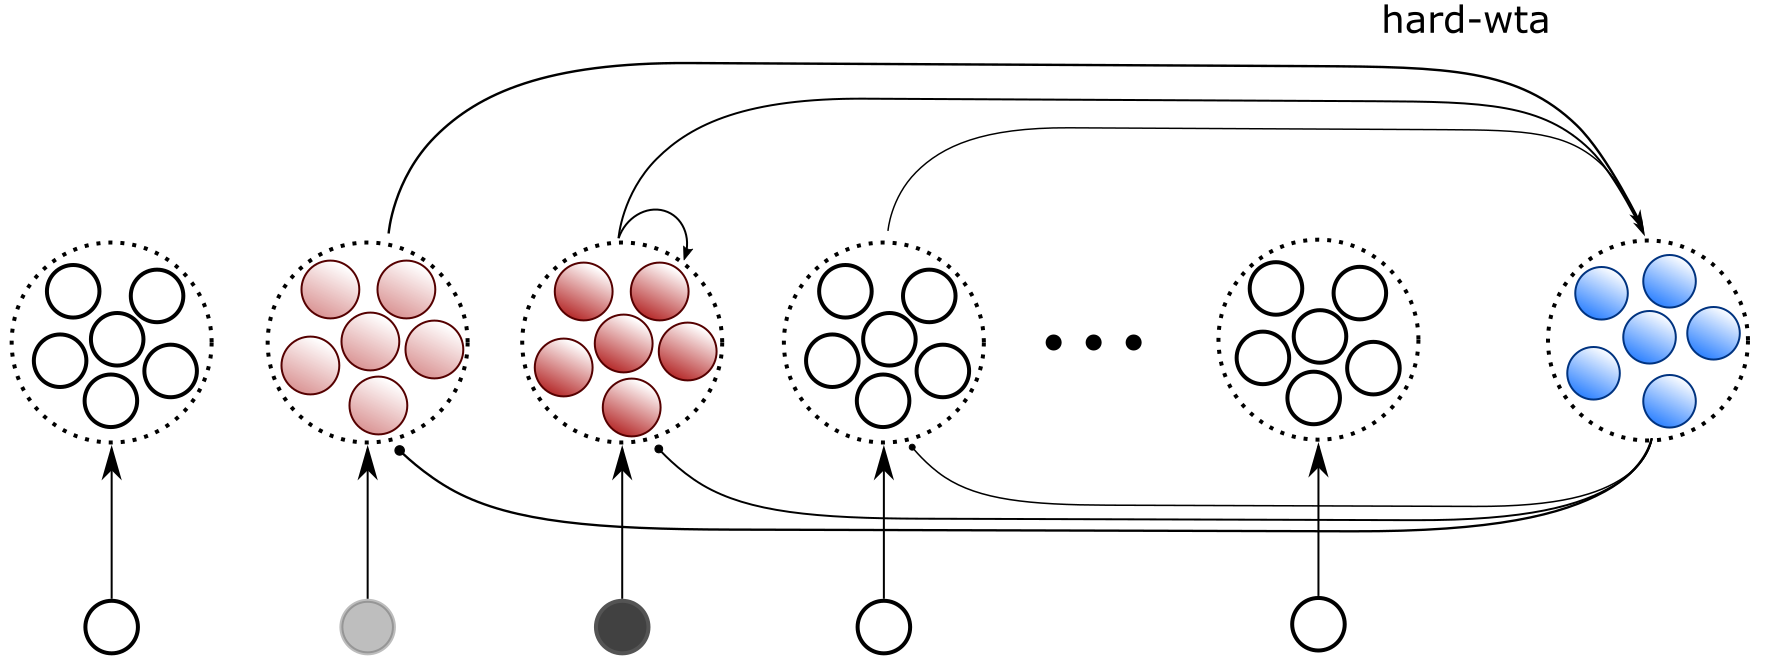
\includegraphics[width=\linewidth]{img/chapter3/hard_wta_global_inh.png}
\caption{}
\label{fig:hard_WTA_global_inh}
\end{subfigure}
\begin{subfigure}{.4\textwidth}
\centering
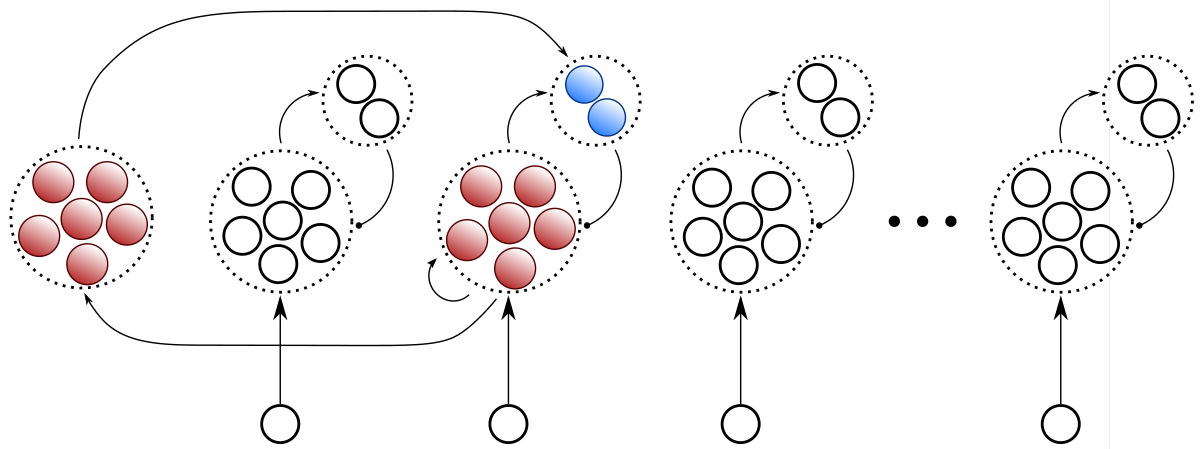
\includegraphics[width=\textwidth]{img/chapter3/hard_wta_global_exc.png}
\caption{}
\label{fig:hard_WTA_global_exc}
\end{subfigure}
\caption[Two Hard Winner-take-all network sketches]{Two Hard Winner-take-all network architectures. Panel (\subref{fig:hard_WTA_global_inh}) shows a network of excitatory clusters of LIF neurons with in-cluster recurrent excitatory connections and a global inhibitory population receiving input from all of the excitatory clusters and providing uniform inhibitory feedback to all of them proportionally to their collective activity. }
\label{fig:hard_wta_sketch}
\end{figure}

\begin{figure}[p!]
\centering
    \begin{subfigure}{.33\textwidth}
        
        \includesvg[width=\textwidth]{img/chapter3/activity_global_inh.svg}
       \caption{}
        \label{fig:activity_global_inh}
    \end{subfigure}
    \centering
    \begin{subfigure}{.37\textwidth}
        
        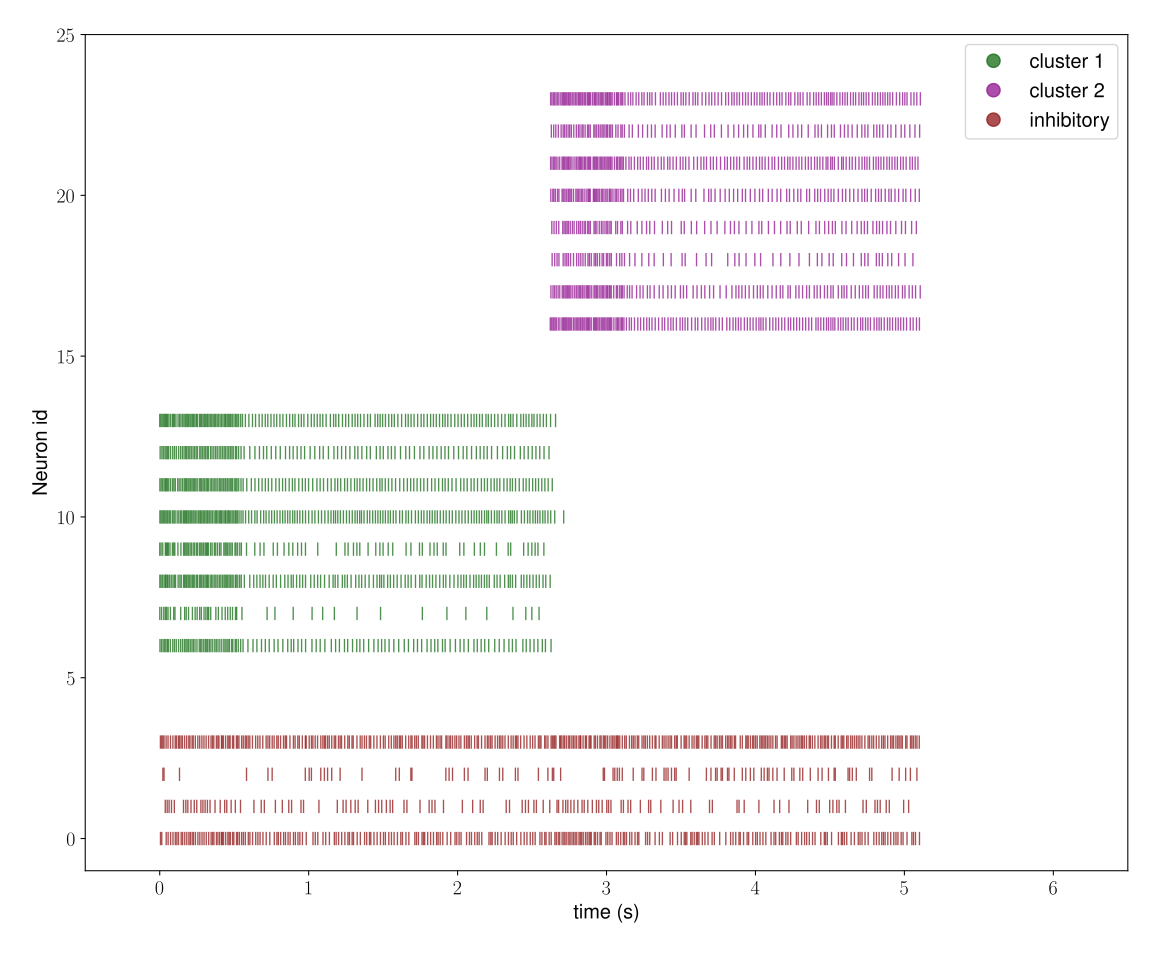
\includegraphics[width=\textwidth]{img/chapter3/raster_global_inh_hard_wta.png}
        \caption{}
        \label{fig:raster_global_inh}
    \end{subfigure}
    \hfill
    \centering
    \begin{subfigure}{.35\textwidth}
        \includesvg[width=\textwidth]{img/chapter3/activity_local_inh.svg}
        \caption{}
        \label{fig:activity_global_exc}
    \end{subfigure}
    \centering
    \begin{subfigure}{.35\textwidth}
        \includesvg[width=\textwidth]{img/chapter3/raster_local_inh.svg}
        \caption{}
        \label{fig:raster_global_exc}
    \end{subfigure}
    \caption[\ac{hWTA} network examples with local and global inhibitory activity]{\ac{hWTA} examples with local and global inhibitory activity, as shown in the Figure~\ref{fig:hard_wta_sketch}. In both cases, the population firing rate plots (on the left) and the firing raster plots (on the right) show 2 seconds of steady sustained balanced activity induced by a 0.5 second input in one cluster, followed by 0.5 seconds of input to cluster 2 which leads to a state switch, with feedback inhibition eliminating activity in the first cluster.}
    \label{fig:hard_wta_dynapse_recordings}
\end{figure}

%A benchmark experiment used for parameter search is designed as follows \dz{REF: Maryada's simulation work, our shared ZNZ poster}:

%\dz{PLOT TO ADD: Introduce the transition from cluster A to cluster B while preserving self-sustained activity.}

Figure~\ref{fig:hard_wta_dynapse_recordings} shows the state transition between two clusters following a delayed input for both configurations with global inhibition and local inhibitory clusters. The architecture preserves a single winner, implementing competitive behaviour between the clusters while preserving the persistent activity of the winner in the absence of input under control. 

%\dz{Discuss how the activity is much more balanced with global EXC, while the input vs steady activity is higher for global INH}

\newpage
\subsection{Using soft Winner-take-all networks.}
\label{sec:sWTA}

Figure~\ref{fig:global_inh_wta_sketch} shows an example of a network implementing both cooperation and competition: cooperation is mediated by excitatory connections with local connectivity (nearby clusters are connected via excitatory connections), and competition is achieved by means of global inhibitory connections: all clusters are inhibited by the population of inhibitory neurons, which are stimulated by the excitatory neurons of all the clusters in the network.
These types of networks are often referred to as \ac{sWTA} networks.
In these networks, nearby neurons are biased to have similar response properties (e.g., similar stimulus preferences, or receptive fields) and thus create a map in which close-by units represent similar features.


\begin{figure}[h]
\centering
\begin{subfigure}{.45\textwidth}
\centering
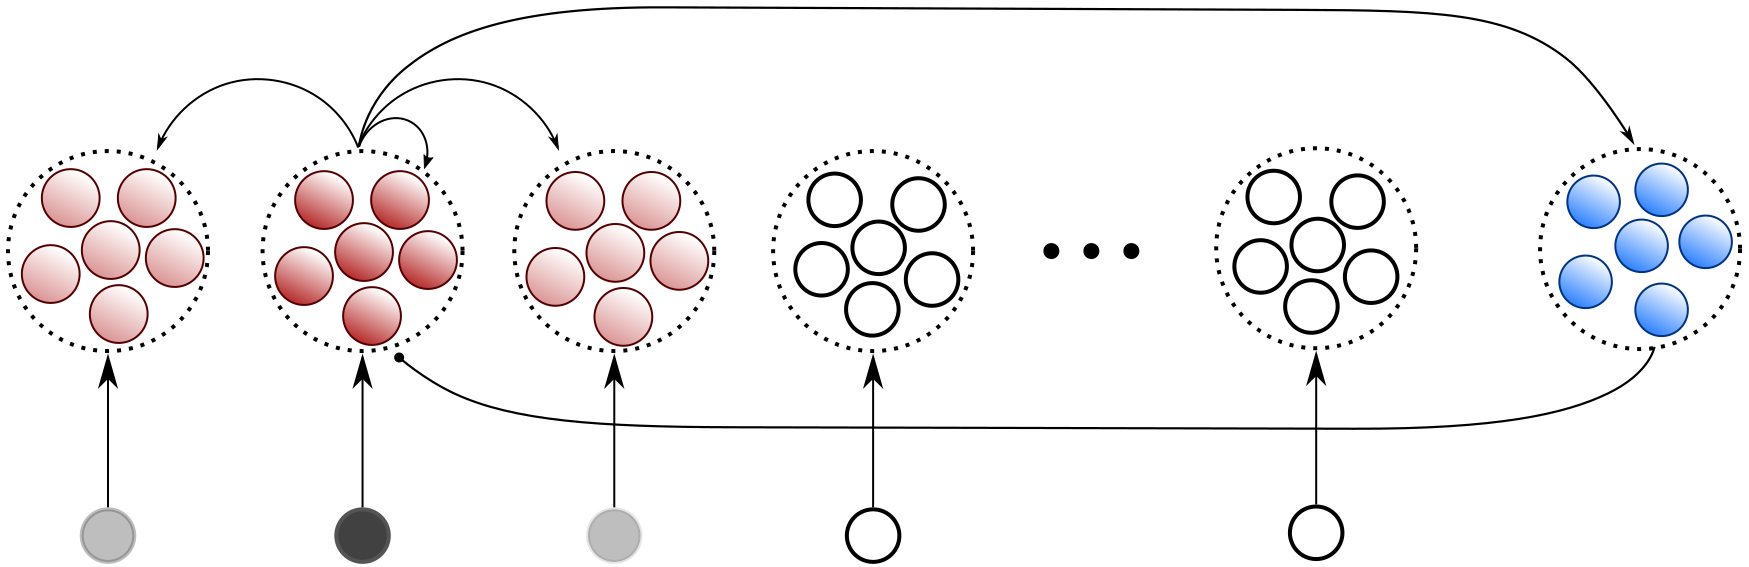
\includegraphics[width=\linewidth]{img/chapter4/position-wta.png}
\caption{}
\label{fig:global_inh_wta_sketch}
\end{subfigure}
% \begin{subfigure}{.49\textwidth}
% \centering
% \includegraphics[width=.9\linewidth]{global_exc_WTA_sketch}
% \caption{}
% \label{fig:global_exc_wta_sketch}
% \end{subfigure}\\
\begin{subfigure}{.5\textwidth}
\centering
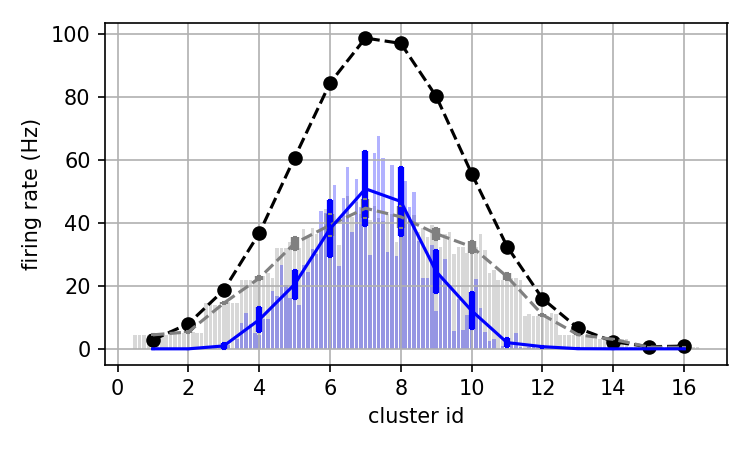
\includegraphics[width=\textwidth]{img/chapter3/16_clusters_ff_and_global_INH_bars_blue.png}
\caption{}
\label{fig:bump_global_inh_WTA}
\end{subfigure}
% \hfill
% \begin{subfigure}{.49\textwidth}
% \centering
% \includegraphics[width=\textwidth]{fig_clustered_WTA/16_clusters_global_exc}
% \caption{}
% \label{fig:bump_global_exc_WTA}
% \end{subfigure}
\caption[Population code in a soft Winnter-Take-all network. Population code sharpening.]{Example of a competitive network comprising multiple clusters coupled via local excitation and global inhibition; (\subref{fig:global_inh_wta_sketch}) network diagram of the network which comprises 16 clusters of 8 excitatory neurons each and a global inhibitory cluster of 20 neurons. Input nodes stimulate all neurons in the cluster with equal strength; input rates are spatially distributed (shades of gray); neurons in each cluster have all to all recurrent connections (not shown in the diagram) with 100\% connection probability; neurons of neighboring clusters are connected with a 10\% probability; excitatory to inhibitory neurons have a 20\% connection probability and inhibitory to excitatory neurons have an 80\% connection probability.
  (\subref{fig:bump_global_inh_WTA}) network activity measured experimentally from the chip in response to a Gaussian input bump of Poisson spike trains with a mean amplitude of 100Hz (black dashed line). The gray dashed line represents the response of a pure feed-forward network without recurrent excitatory and inhibitory connections. The solid blue line represents the competitive network response, with recurrent excitation and global inhibition activated. The error bars in this data reflect the variability within clusters. The vertical bars of both gray and blue plots represent the responses of the individual neurons in the cluster.}
\label{fig:bump_coupled}
\end{figure}

Depending on their parameters, the same \ac{sWTA} network can be used to process continuous signals and represent different features that change smoothly in feature space (e.g., the orientation of a visual stimulus) or to manipulate discrete symbols such as numbers and numerable variables (e.g., one of n possible keywords).
The recurrent connections in the network make the outputs of individual clusters depend on the activity of the whole network, and not just on the neurons driven by the local input~\cite{Douglas_etal95}.
As a result, \acp{sWTA} can perform both linear operations, such as amplification by a linear gain or locus invariance, and complex non-linear operations, such as normalization, selective amplification and non-linear selection, multi-stability, or signal restoration~\cite{Douglas_Martin07}.
Interestingly, it has been observed that, despite significant variation across cortical areas, \ac{sWTA} types of connectivity patterns are found throughout all of the neocortex~\cite{Douglas_etal89,Douglas_Martin04}.
Indeed, this architecture is a ``canonical microcircuit'' that can be used as a fundamental computational primitive for multiple types of both signal processing and computing tasks~\cite{Douglas_Martin07}.
It has been shown that the computational abilities of \acp{sWTA} are of great importance in tasks involving feature-extraction, signal restoration and pattern classification problems~\cite{Maass00}.
Artificial neural networks with this architecture, and their neuromorphic hardware implementations, have been used to detect elementary image features (e.g., oriented bars) and reproduce orientation tuning curves of visual cortical cells~\cite{Ben-Yishai_etal95,Somers_etal95,Chicca_etal07a}.

\paragraph{Tuning curve sharpening.}
Figure~\ref{fig:bump_global_inh_WTA} shows the experimental measurements from the \ac{sWTA} network formed by the silicon neuron circuits of the DYNAP-SE chip, with (blue solid line) and without (gray, dashed line) the recurrent connections.
The black dashed lines in Fig.~\ref{fig:bump_global_inh_WTA} represent the input to the network.
As for Fig.~\ref{fig:bump_decoupled}, the output firing rate of the silicon neurons is kept low via the refractory period setting to reduce power consumption. So while low frequency inputs are followed faithfully, high frequency ones are scaled to lower values.
However, what is important is the effect of the recurrent inhibition: this network of silicon neurons can reproduce the selective amplification features expected from \acp{sWTA} models, amplifying with a gain higher than one of the strongest inputs while at the same time suppressing the weaker ones.
This gives rise to a ``sharpening'' of the tuning curve similar to what has been measured in real cortical cells~\cite{Ben-Yishai_etal95,Douglas_etal95,Anderson_etal00,Indiveri_etal09}.
\begin{figure}[h]
\begin{subfigure}{.32\textwidth}
\centering
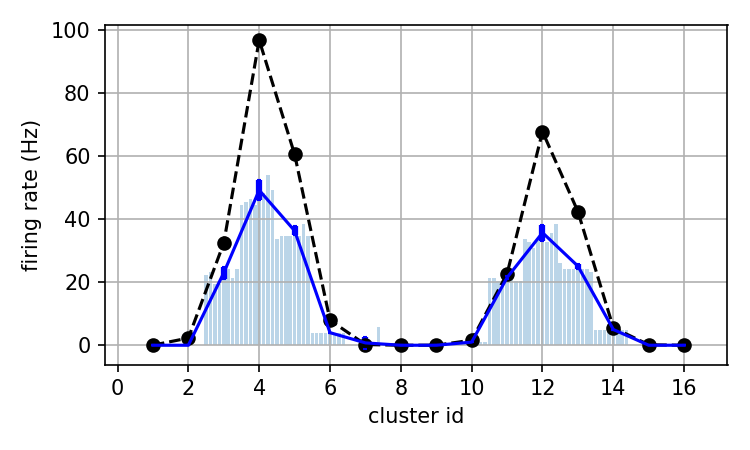
\includegraphics[width=\linewidth]{img/chapter4/selective_amplification_ff.png}
\caption{}
\label{fig:selective_amplification_ff}
\end{subfigure}
\hfill
\begin{subfigure}{.32\textwidth}
\centering
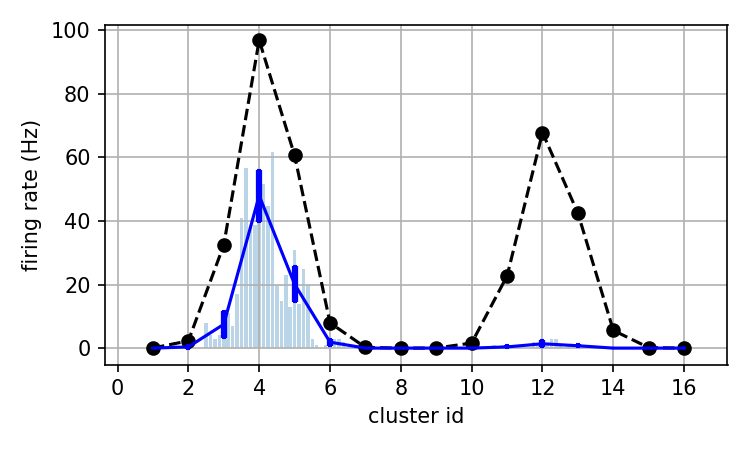
\includegraphics[width=\linewidth]{img/chapter4/selective_amplification_inh_WTA_L3.png}
\caption{}
\label{fig:selective_amplification_l}
\end{subfigure}
\hfill
\begin{subfigure}{.32\textwidth}
\centering
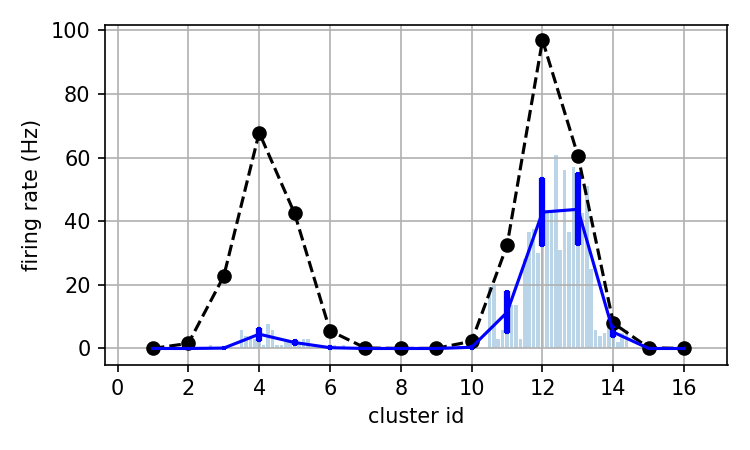
\includegraphics[width=\linewidth]{img/chapter4/selective_amplification_inh_WTA_R2.png}
\caption{}
\label{fig:selective_amplification_r}
\end{subfigure}
\caption[Population code selective amplification]{When provided slightly different inputs (two bumps with amplitudes of 100Hz and 70Hz), the \ac{sWTA} network of Fig.~\ref{fig:bump_coupled} selects the strongest one.  Panel (\subref{fig:selective_amplification_ff}) shows the network's pure feed-forward response when both recurrent excitatory and inhibitory connections are disabled. The dashed line and solid circles represent the input firing rates; the solid blue lines represent the activity averaged over clusters of 8 neurons each; the histograms represent the firing rate of individual neurons. Panels (\subref{fig:selective_amplification_l}) and (\subref{fig:selective_amplification_r}) show the response of the network when the recurrent connections are activated: a stable output activity bump forms around the location of the stronger input, while the response to other input is almost completely suppressed.}
\label{fig:selective_amplification}
\end{figure}

\paragraph{Selective amplification.}
Due to their cooperative/competitive nature, clusters with the highest response are amplified while weaker ones are suppressed.
To highlight the selective amplification properties of the \ac{sWTA} presented in Fig.~\ref{fig:bump_coupled} we stimulated the network with two input bumps of slightly different amplitudes.
Figure~\ref{fig:selective_amplification} shows the response of the network to these inputs.
%The interplay of positive and negative feedback in the network results in selective amplification of only one \dz{(stronger)?} of the inputs.
The reference response of the feed-forward network without the recurrent feedback is shown in Fig.~\ref{fig:selective_amplification_ff}. As expected, the network follows the input with two bumps of the same width and proportional amplitudes.
As soon as feedback is enabled, the non-linear processing features of the network become evident: higher inputs are preserved and ``pass through'' to further processing stages, while (even slightly) weaker inputs are almost fully suppressed (see panels~(\subref{fig:selective_amplification_l}) and (\subref{fig:selective_amplification_r}) of Fig.~\ref{fig:selective_amplification} for the cases in which the stronger input is on the left or right side, respectively).

\paragraph{Signal restoration.}
These very same features enable the network to support another important computational primitive: that of ``signal restoration''.
This is the very process that allowed the success of logic gates in digital computing systems, always restoring their output to a nominal ``1'' level or ``0'' level.
If signals are encoded with distributed population codes as provided by the output of \ac{sWTA} networks, then multiple layers of such networks automatically carry out signal restoration. To demonstrate this experimentally, we provided in input to the hardware \ac{sWTA} network a  ``bump'' signal as produced by neurons belonging to another \ac{sWTA} network, and corrupted it in two different ways: with ``dead'' neurons (i.e., by silencing completely 30\% of the input units) and with corrupted inputs (i.e., by adding 20\% Gaussian distortion to the nominal value of each input unit). As shown in Fig.~\ref{fig:pop_code_robustness} the network is able to recover the original population encoded signal and produce an output that is very close to the un-corrupted input. 

\begin{figure}[h]
\centering
\begin{subfigure}{.48\textwidth}
\includegraphics[width=\linewidth]{img/chapter4/example_distorted_bump.png}
\caption{}
\label{fig:resoration}
\end{subfigure}
\hfill
\begin{subfigure}{.49\textwidth}
\includegraphics[width=\linewidth]{img/chapter4/sWTA_normal_noise_example2.png}
\caption{}
\label{fig:bump_noise}
\end{subfigure}
\caption[Population code Signal restoration]{Signal restoration demonstration. The setup is identical to Fig.~\ref{fig:bump_coupled}. (\subref{fig:resoration}) response of the network to an input bump  with 30\% of rate inputs missing completely. (\subref{fig:bump_noise}) response of the network to an input corrupted by 20\% Gaussian additive distortion. The solid black line shows the perturbed input overlaid over the gray ideal input and response. In both cases, blue curve shows the response of clusters of the network. The blue error bars indicate SD within each cluster. The blue histogram bars show activity of individual neurons. In both cases, the resulting activity bump location still represents the intended population code.}
\label{fig:pop_code_robustness}
\end{figure}

\paragraph{Attractor dynamics.}

\acs{sWTA} networks can exhibit dynamic characteristics of attractors underlying many cognitive functions, including decision making and working memory. 
Depending on their connectivity patterns, \ac{sWTA} networks can open boundary conditions (e.g., to represent a variable ranging from zero to a maximum value) or closed boundary conditions (e.g., representing an angle that can take values between 0 and 360$^\circ$).
In the latter case, the \ac{sWTA} network forms a ring attractor, rather than a line in the network state space.
Both types of configurations have been found in different brain areas (e.g., in the brain stem for oculomotor control~\cite{Seung98}, or in the fly's central complex for navigation~\cite{Lyu_etal22,Kim_etal19a}).


\begin{figure}[h]
\centering
\includegraphics[width=0.99\linewidth]{img/chapter3/global_inh_drift3_bump_drift.png}
\caption[Population code drift in absence of input.]{Population code follows the input and then drifts freely when no input is presented. A WTA network identical to Fig.~\ref{fig:bump_coupled} receives two population coded inputs with a 1-second length (red lines). The network activity (blue spikes) is focused by input, and then begins to drift when the input is removed. Black dashed line shows the population vector (the population coded value) estimated every 20 ms. Grey horizontal lines illustrate the division of neurons into clusters of 8.}
\label{fig:bump_drift}
\end{figure}



In both types of networks, the position of the neuron, or cluster of neurons, that has the highest activity represents the value of the variable being encoded.
When driven by external signals, this activity bump stabilizes around the strongest input. Ideally, when the input is removed, and when the sWTA is configured to produce working memory behavior, the activity bump  should persist and remain in the same position. However, in our experiments, after the input is removed, the bump of activity starts to drift (see  Fig.~\ref{fig:bump_drift}). In these experimental results, the \ac{sWTA} activity bump drifts randomly, continuously shifting between semi-stable positions across the whole population for the first two seconds of the recording. At $t=2\,s$ an input bump is presented with a Gaussian profile. The peak of the Gaussian is indicated by the red line in  Fig.~\ref{fig:bump_drift}. As evidenced, the network activity quickly shifts to the strongest input's location and stays there until the next input is presented. After the input is removed again (at $t=4\,s$) the bump starts to drift again. Thus, this sWTA does not have a single, strong attractor able to immediately cancel the memory of an input. 
This phenomenon has been modeled also in theoretical works, and has been shown to be controllable by endowing the network with homeostatic plasticity features~\cite{Renart_etal03a}, which can be readily implemented in neuromorphic electronic circuits~\cite{Qiao_etal17,Bartolozzi_Indiveri09}

\subsection{Linking multiple soft Winner-Take-All networks together}
\label{sec:relnets}

\ac{sWTA} networks have been associated with canonical microcircuits that sub-serve many computational properties in many cortical areas~\cite{Bastos_etal12,Carandini_Heeger12,Jonke_etal17}. As these microcircuits have been found often to be reciprocally connected in the cortex~\cite{Binzegger_etal09}, it is natural to hypothesize that multiple \ac{sWTA} networks coupled among each other have the potential of performing even more complex computations.

\begin{figure}[b!]
  \centering
  \begin{subfigure}{.38\textwidth}
    \includegraphics[width=\linewidth]{img/chapter5/threeway_hardwired.png}
    \caption{}
    \label{fig:rel_net_arch}
  \end{subfigure}
  \hfill
  \begin{subfigure}{.49\textwidth}
    \includegraphics[width=\linewidth]{img/chapter5/threeway_raster.png}
    \caption{}
    \label{fig:rel_net_rast}
  \end{subfigure}
    \caption[Relational network example.]{(\subref{fig:rel_net_arch}) Relational network implementing the relation A+B=C with three coupled 1D \ac{sWTA} networks via a 2D hidden population H. (\subref{fig:rel_net_rast}) Raster plot of input variable populations A, B, changing over time, and output variable population C continuously holding the relation.}
  \label{fig:rel_net}
\end{figure}

Indeed, it has been shown how these coupled networks can form arbitrary relations between the variables encoded in the individual \ac{sWTA} populations~\cite{Cook_etal10}, or can self-organize to learn relations when coupled and endowed with spike-based learning mechanisms~\cite{Diehl_Cook16}.
One example of a relational network formed by coupling multiple population-coded variables among each other is the model of sensory-motor mapping between head and eye positions~\cite{Deneve_etal01}.
Another example of a relational network is shown in Fig.~\ref{fig:rel_net}, where three \ac{sWTA} networks are coupled to form the relationship $A+B=C$~\cite{Cook_etal10,Zhao_etal20}.
The neuromorphic implementation of this relational network consists of 4 distinct populations of silicon neurons: three input 1D \ac{sWTA} networks, representing the variables $A, B,$ and $C$, and one hidden 2D population encoding the relationship between the three variables (see Fig.~\ref{fig:rel_net_arch}). The links from the 1D networks to the 2D one are bi-directional, therefore creating a recurrent network that allows the activity of 1D networks to influence the others. We configured the hardware such that the variables encoded by the networks range from 0 to 1, and we implemented closed boundary conditions such that the variables are wrapped around (i.e., if an operation increases a variable by $n$ beyond 1, the result is only the fractional part of $n$). The plots of Fig.~\ref{fig:rel_net_rast} show experimental data measured from the silicon neurons representing the different networks, as populations $A$ and $B$ were being driven by external inputs.
The choice of the relationship used to demonstrate this principle was arbitrary.  Furthermore, in this example we set the parameters of the networks (and in particular the weights of the hidden population) manually, to demonstrate the proper operation of the relationship chosen. It is interesting to note though that arbitrary relationships, including non-monotonic ones, such as $A^2 + B^2 = C^2$, can also be trained through local spike-based learning rules~\cite{Jug12,Diehl_Cook16}. A hardware-implemented example of a relation learning process is shown in Chapter ~\ref{ch:EXAMPLES} of the thesis.


\subsection{Temporal coding: oscillators and delay chains}


%\dz{Revisit this section:}
%\dz{Add references about the temporal coding.}
%\dz{Delay chains for sound localization in barn owls~\cite{Carr_93}, and~\cite{Carr_Konishi90} ~\cite{Ashida_15}, also Moritz and Germain's CapoCaccia prototype etc.}

%\dz{Abeles: synfire chain basics, synchronous and asynchronous volley activations, the concepts of polychronization from Izhikevich and absence of synaptic delays on DYNAP-SE1. CAVIAR chip delay lines example.}

All the way until now, we have discussed representations in the spiking networks that rely on steady firing, and we assumed that the variable represented is most likely some state of the environment or our agent in that environment. By taking interest in only momentary rates of the neurons, we neglect the property that is natively embedded in the spiking neuron's dynamics: time.

Unlike artificial neural networks, with spiking neurons and current-based synapses we have time playing part at every level of computation: the events take time to travel from source to destination, the synaptic potentials have time-evolving profile that is in turn integrated by the neurons. To estimate firing rates we once again integrate the events within some window. The timing of two input spikes defines whether the postsynaptic neuron will fire or not. All this means, that we could use some of these domains to encode some information.

Indeed, temporal coding in the brain is widely theorised, and there exist various network models of spike-based temporal representations. Notably, some of them we could obtain just by looking at our previously configured networks of excitatory and inhibitory clusters differently.

\begin{figure}[h!]
  \centering
  \begin{subfigure}{\textwidth}
    \includegraphics[width=\linewidth]{img/chapter3/delay_chain_sketch.png}
    \caption{}
  \end{subfigure}
    \caption[Delay chain sketch]{Delay chain sketch. A series of excitatory clusters of the same size connected reciprocally within themselves and to their next neighbour create a chain that propagates an activity pulse along with constant speed. A feedback inhibitory connection to the previous cluster ensures that it does not stay active after the pulse has been passed on. The speed of the pulse moving along the chain depends linearly on the mean excitatory weight (given that all of the excitatory weights in the network are set as equal). Such a network can hold a temporal pattern of pulses and preserve delays between them, with memory limitation being its length.}
  \label{fig:delay_chain_sketch}
\end{figure}

For instance, if we take a look at how firing activity propagates between the clusters as a population bump drifts in the absense of input on Fig.~\ref{fig:bump_drift}, we can see that it is indeed not instantaneous. This activity propagation delay, originating from synaptic and neuronal integration, could be used for time encoding. If in a line of excitatory clusters we remove connections to the relative left neighbour of every cluster, any spiking activity of one cluster would pass onto the one on the right. To avoid the always-on self-sustained firing we could also create an inhibitory interneuron that would kill any activity of the cluster to left. The result is a chain of clusters, where activation would move in one direction, until the end of the chain, as shown in Figure ~\ref{fig:delay_chain_sketch}.

These structures are commonly referred to as delay lines or synfire chains~\cite{Abeles91} and convert the dimension of time into the dimension of space. Given that all neurons and connections have identical parameters, a pulse of activity would propagate along the chain with constant speed. The feedforward excitatory weight (or weight bias, in the case of the DYNAP-SE1 chip) controls the synaptic pulse amplitude, which in turn controls the delay before the postsynaptic neuron fires. This way, a single parameter would control the speed of the pulse along the chain.

In the Section~\ref{sec:delay_lines}, we discuss the delay line properties in more detail, specifically configured on the DYNAP-SE1 chip.

%\dz{Delay chain memory capacity. Time resolution. Once encoded, the memory doesn't fade}
%Here comes an obvious trade-off between the temporal resolution of the input and its length. By using what is essentially binary units to represent time steps, the input pattern is limited to 



The delay chain mechanism could be applied to a wide variety of scenarios involving detection or generation of precisely timed events, such as spatial localization or generation of complex movements. The generated movements also can be periodic if the delay chain is looped creating a spiking oscillator. The work of Chenxi Wu and Renate Krause~\cite{Krause_etal21} shows an example of an on-chip 3-state oscillator serving a pattern generator. A longer chain with multiple loops and some outward branches could generate a very complex temporal structure in the output.

The delay chain sheet can also have a digital classifier listening to all neurons at once. It has been demosntrated on DYNAP-SE1 chip specifically for the ECG signal~\cite{Gerber_etal22}.

In the temporal coding field, variable synaptic delays are a quite common strategy, while the hardware implementation in analog circuits is not trivial and requires additional chip area. To some extent, the solution with chains of clusters resolves this issue by using more neuron units for variable delay pathways.

%\dz{Discussion - in many frameworks synaptic delays play a big role. One might come up with a strategy to use variable length delay chains.}

\section{Discussion}

In this chapter we have discussed the power of distributed representations. It seems that the excitatory-inhibitory balance that enables population bump sharpening (or, specifically, the recurrent excitation) plays a significant role in the overall smooth bump shape regardless of its position around the ring attractor. If we look at the decoupled bump activation of the same population of neurons, we see that response rate heterogeneity is non-negligible.
Tackling the same problem on a different chip, Emre Neftci proposed a mismatch compensating algorithm through activity-based weight sorting~\cite{Neftci_Indiveri10}. This ensured the smoothness of the bumps in the WTA structure in that case. The advantage of our method is in the independence from the exact neurons the network is applied to, as we do not have to fine-tune our connectivity matrix for the specific mismatch profile.\\

A future development direction in this chapter is the automation of the EI balance tuning. Currently, despite having the theoretical guidelines for balancing the WTA, hand tuning was still needed to get the network to exhibit all of the demonstrated behaviours. In fact, from experience, selective amplification setting proved to be the one having the most narrow parameter range. Some attempts have been done by Maryada and me to grid search the parameter space of the recurrent excitatory, recurrent inhibitory and feedforward weights, but they were not very indicative.\\

Another observation we made here is the stability of the static networks against the temperature fluctuations. As shown in the previous chapter, the mean distributions of individual parameters may move as much as one sigma between night and day time. The once saved settings for the sensitive selective amplification experiment always resulted in the same reproducible behaviour, which is surprising.\\

One of the next steps in complexity for the presented static network prototypes (and the software block) can be reproduction of the multi-variable Neural State Machine and constraint satisfaction problem~\cite{Neftci_etal12a}. It is interesting to see if our results make the tuning and configuration of such networks easier.




\newpage

\chapter{Enabling long-term structural changes. Dynamic connectomes.}
\label{ch:dynamic_connectome}

In this section, we increase the complexity of the system by implementing a mechanism for long-term structural changes, enabling learning. These lasting changes are crucial for any environmental adaptation we want our system to do. This also serves as an alternative strategy for coping with the device parameter variability.

In neural network models, following the biological evidence, these structural changes are primarily implemented with permanent changes of connection efficacies, or, for \ac{SNN}s, synaptic weight updates. Indeed, the principle of functional learning through inter-neuron connection weight updates in biological networks has been widely demonstrated \emph{in vivo} as well as \emph{in vitro} through synaptic growth, transformations and pruning~\cite{George18}.
Moreover, the way these weights are updated plays a fundamental role in what function the network will or will not be able to learn. Thus, the choice of the appropriate learning rule determines the possibility of capturing and extracting the relevant features in the input stream fed to the network. At the same time, while mathematically we can engineer a multitude of options, both biological and hardware constraints help us limit our variety of solutions. While ANNs tend to employ (to the great success~\cite{Sejnowski20}) global weight update strategies such as output error backpropagation, where individual weight increments can only be calculated synchronously and with access to the entire weight matrix at once, the biological synapse conductance is largely driven by the correlated pre- and postsynaptic activity, only vaguely depending on the global network state. On the hardware side of things, centralized approaches burn a lot of energy gathering centralized information about the entire system to make the update step. Biology tends to save the limited resources as much as possible, and local information processing is a direct result of that.

By design, the DYNAP-SE1 chip does not have any synaptic plasticity. However, we can exploit the nature of its asynchronous routing mechanism that does not interrupt the spiking dynamics, to perform some dynamic connectivity changes.

In this chapter, I introduce a hardware-constrained local spike-based so-called ``neo-Hebbian''~\cite{Gerstner_etal18} reward-gated STDP learning rule and additional regulatory mechanisms fitting the considerations above and show its implementation for the \ac{DYNAP}-SE1 chip. The learning rule fits the chip's routing architecture as, while being spike-based, it only applies cumulative updates. Given the low precision of the weight on the chip, a heavy stochastic quantization method is applied, which also introduces a computational advantage serving as a built-in exploration mechanism. Since the updates are calculated externally to the chip, we argue that such approach could be used for testing any alternative learning rules as long as the meet the criteria of sparsity of the weights and cumulative non-frequent updates.

This resulting learning framework is then applied in conjunction with the static network structures introduced in the previous chapter to demonstrate biologically plausible examples of learning in an on-chip network of spiking neurons (see Chapter~\ref{ch:EXAMPLES}).


\section{Revisiting neuromorphic routing. Weight multiplexing. Chip-in-the-loop discussion.}

To find the matching learning rule applicable to our hardware case, we need to revisit the connectivity constraints of our chip.

On DYNAP-SE1 chip, communication between hardware spiking neurons is implemented via the \ac{AER} protocol ~\cite{Sivilotti91, Deiss_etal94, Boahen00}: the system of asynchronous hierarchical digital routers transfers an ``event'' - a single packet of data containing the timestamp of the occurrence of the event (spike), and the address of the source neuron that emitted that spike~\cite{Moradi_etal18}.
The \ac{AER} event is registered by the router at the moment of occurrence at the neuron and is broadcast to all synapse circuits of all neurons of the target chip(s). The routing information is stored in two parts: (i) the emitting neuron circuit has a dedicated \ac{SRAM} cell that defines which target \emph{chips} the event is broadcast to; (ii) every neuron has 64 10-bit \ac{CAM} registers defining spikes from which neurons should be accepted as source. In case of the matching source neuron ID (identical to the one written in the CAM cell), the chain of the dedicated pulse generator (PG) and the pulse extender (PE) blocks induces a current in the respective analog DPI synapse circuit (illustrated in Figure~\ref{fig:dynapse_AER_block}).

\begin{figure}[h]
  \centering
    \includegraphics[width=.9\textwidth]{img/chapter4/dynapse_neuron_block_diagram.png}
    \caption[AER processing block of one neuron of the DYNAP-SE1 core]{Neuronal AER processing block, Figure 9 in~\cite{Moradi_etal18}, showing the chain of circuits generating a PSP upon receiving the matching source AER event.}
  \label{fig:dynapse_AER_block}
\end{figure}


The central principle we need to note here is what happens when multiple CAM cells are programmed to hold the same source neuron address. The respective PG-PE chains will be triggered simultaneously, generating fully aligned EPSPs/IPSPs on the same neuron, depending on the synapse type set in the CAM cell. And if the selected types are identical, it will indeed be the very same physical analog synapse circuit processing the same input event multiple times. Since these chains act independently, the resulting effect on the DPI synaptic circuit is additive, which we can use for multiplexing (i.e. selectively multiplying, and thus controlling) the individual functional weights (efficacies) between the pairs of neurons while the analog continuous \emph{weight biases} are still shared between all same-type synapses of the core.

\begin{figure}[b!]
  \centering
    \includegraphics[width=.7\textwidth]{img/chapter4/CAM_multiplexing.png}
    \caption[Multiplexing CAMs for quantized weight control]{Automated and time-synchronized measurement of an AMPA EPSP generated by a single input spike with multiple CAM cells listening to the same input neuron, effectively creating duplicate parallel connections between the two neurons. The measurement shows that, at first, the amplitude of the first peak increases linearly with the number of parallel AMPA connections but then saturates at higher values.}
  \label{fig:CAM_multiplexing}
\end{figure}

To verify and characterize this mechanism, we look at the EPSP shape when measuring the neuron membrane voltage, as the direct observation of synaptic behaviour is unavailable on the DYNAP-SE1 chip. To observe the approximate shape of the EPSP, we once again set the neuron circuit leak to the maximum value to eliminate any synaptic input integration. 


Figure~\ref{fig:CAM_multiplexing} shows a measurement from a postsynaptic neuron receiving a spike through multiple CAM cells listening to the same input neuron, routed through an AMPA DPI synapse. The pulses arriving through parallel CAM blocks are summed up at the synapse circuit, adding to the amplitude of the resulting EPSP. The increments of the EPSP amplitude are dependent on the synapse circuit weight bias, while the DPI threshold bias controls the maximum amplitude that the EPSP would never exceed. At first, the EPSP amplitude increments are constant (i.e. the PSP amplitude scalers linearly), but are then reduced and eventually saturate with more than 8-10 parallel connections.


This gives us some understanding of how rough is our control over individual weights on the chip (i.e. 3-bit weights effectively). On top of this, since each neuron has only 64 CAM cells in total, using multiple of them takes away from the total number of possible inputs of the neuron. Indeed, these multi-CAM profiles are still different for different physical DPI circuits due to variability through mismatch.

%\subsection{Global vs local updates, in the loop.}

%\dz{Single-weight vs batched connectivity matrix updates, show why batched updates are favoured for our case.}
%\bigskip
%\dz{Fusi learning rule, Machens learning rule and applicability.}
%\bigskip
%\dz{Mention transfer learning, He Xu's 2019 Capocaccia with the first chip in the loop attempt.}
%\bigskip



\subsection{Weight quantization}

Several extra steps must be taken to perform the weight changes on the DYNAP-SE1 chip. The weight matrix on the chip can be reprogrammed without interrupting the neural activity; however, no learning rules can be enabled on the chip itself. Moreover, the true weight value of one synapse created between the two neurons is determined by the analog bias shared by design of chip layout between all synapses of this type in the given core. As shown above with the EPSP scaling measurement, individual \textit{effective weights} can be set by creating multiple \textit{parallel} synapses between the pair of neurons, which results in their low, or quantized, precision.\\

\begin{figure}[b!]
  \centering
    \includegraphics[width=.7\textwidth]{img/chapter4/chip_in_the_loop_logic.png}
    \caption[Chip in the loop with storage of the precise and quantized versions of weight matrices.]{Chip in the loop weight matrix update logic illustration, with the precise and quantized matrices on the lower panel. The chip router configuration uses the quantized matrix, and thatis the matrix that the physical neurons of the chip interact through. The algorithmic overhead on the PC retrieves the spikes from the chip in a fast loop and updates the precise floating-point weights based on any arbitrary weight update mechanism. The precise matrix then is stochastically quantized when applied to the chip.}
  \label{fig:weight_quantization}
\end{figure}

We implemented an additional quantization step every time the weight matrix was updated and applied to the chip. Inspired by stochastic rounding in fixed precision calculations~\cite{Hopkins_etal20} and an example for limited weight precision ANN training~\cite{Gupta_etal15}, we implemented a similar algorithm for our case.\\

The idea is simple. We introduce the quantization step $\Delta_q$ as a parameter defining the precision of our effective weights. Then we take a weight $w^{ij}_p \in W_p$ and divide it by $\Delta_q$. The two rounding options would be lower $\lfloor \frac{w^{ij}_p}{\Delta_q}\rfloor$ and the higher $\lceil \frac{w^{ij}_p}{\Delta_q}\rceil$ nearest integers values. We round up or down stochastically, by generating a random number between 0 and 1, and comparing it to the fractional part $\{\frac{w^{ij}_p}{\Delta_q}\}$ as a probability to round \emph{up}.

In our framework, we kept two versions of the plastic weight matrix at all times: a matrix of precise weights $W_p \in \mathbb{Q}^{m \times n}$, used for all weight calculations of the given learning rule, and a quantized integer matrix $W_q \in \mathbb{Z}^{m \times n}$, applied to the chip. Conversion from $W_p$ to $W_q$ was done every time the hardware matrix update was required by the learning rule (concept illustrated in Figure~\ref{fig:weight_quantization}).


An additional constraint for the quantization procedure is, of course, the fan-in limit of 64 CAM slots for every neuron. Since we never impose any sparsity on the precise matrix $W_p$, it has to be applied during the quantization procedure. The two obvious strategies are the ``greedy'', when the available CAM slots are attributed to the highest weights first, or the uniform, where the ``ideal'' quantized matrix is uniformly downsampled until it fits (see Figure~\ref{fig:weight_quantization_strategies} for illustration). The figure also illustrates the importance of choice of the quantization step $\Delta_q$, as the increment of the EPSP with each $\Delta_q$ step is equal to the values set by the analog weight bias.

Thus, the full weight update procedure upon the arrival at time on-chip matrix update signal was the following:
\begin{itemize}
    \item New values of precise weights $W_p^{new}$ were calculated based on the old weights $W_p^{old}$ and the updated given by Equation~\ref{eq:reward} using the current values of eligibility traces.
    \item The precise matrix was then $W_p^{new}$ quantized using procedure shown in Figure~\ref{fig:weight_quantization}, creating a matrix of integer values $W_q^{new}$.
    \item The new quantized matrix $W_q^{new}$ was applied to the DYNAP-SE1 chip, creating the corresponding number of logical synapses for each pair of pre- post- neurons.
\end{itemize}

\begin{figure}[t!]
\begin{subfigure}{.4\textwidth}
\centering
\includegraphics[width=\linewidth]{img/chapter4/quantization_greedy.png}
\caption{}
\label{fig:quantization_greedy}
\end{subfigure}
\hfill
\begin{subfigure}{.44\textwidth}
\centering
\includegraphics[width=\linewidth]{img/chapter4/quantization_uniform.png}
\caption{}
\label{fig:quantization_uniform}
\end{subfigure}
\caption[Weight quantization strategies]{Weight quantization strategies applied to sorted input weights of a neuron (each black bar represents the value of the weight, decreasing along the X-axis). These precise values are rounded to the integer levels corresponding to the multiples of parallel connections that the neuron would receive. The weights are stochastically rounded up or down with probabilities equal to their fractional parts. The constraint of limited total input per neuron is addressed with one of the two strategies: \subref{fig:quantization_greedy} The greedy strategy preserves the greatest weights, so the input slots (CAMs) are attributed to the quantized set of weights until the cap is reached; \subref{fig:quantization_uniform} The uniform strategy aims to preserve the entire matrix shape, scaling down the quantized weights uniformly by randomly decreasing one of the input weights by 1 until the cap is reached.}
\label{fig:weight_quantization_strategies}
\end{figure}

%\section{Upcoming hardware solutions for long-term synaptic changes}

%\dz{Add a review about memristors, ferroelectric synapses, other variable conductance devices. Reference a lot of Yigit's work. Reference Charlotte's work, Thomas' and Melika's work.}


\newpage
\section{Reward-gated STDP as a hardware-friendly local learning rule}
\label{sec:RSTDP}

\subsection{Combining STDP with the reward signal}

Reward-modulated spike-timing dependent plasticity (R-STDP) is a popular biologically derived weight update mechanism that bridges together the single spike timing interaction timescale, that is typical for Hebbian synaptic changes\cite{Bi_Poo98}, with the behavioural timescales by the means of long-relaxating synaptic eligibility traces that store cumulative weight updates given by STDP~\cite{Schultz97, Izhikevich07, Fremaux_Gerstner16}. The eligibility traces model the presence of the third (in addition to pre- and postsynaptic spikes) factor in the form of the dopamine signal, effectively gating the weight changes. It is sometimes called neo-Hebbian. R-STDP has been shown to be effective for both more classical feedforward SNN training~\cite{Mozafari_etal18} and biological behavioural experiments, especially where loss-function gradients do not apply~\cite{Izhikevich07,Vasilaki09,Gerstner_etal18}.

In this section, we show how the dynamic routing architecture of the DYNAP-SE1 chip fits this cumulative update property.

%\dz{Add references from the Spinnaker and Brainscales RSTDP implementations}\\

%\dz{TAKEN FROM SPINNAKER PAPER, NEEDS REWRITING OR REFERENCING: The reward mechanism in R-STDP is biologically inspired: the phasic activity of dopamine neurons in the brain was found to encode expected reward (Schultz et al., 1997; Hollerman and Schultz, 1998; Bayer and Glimcher, 2005) and dopamine concentration modulates STDP (Pawlak and Kerr, 2008; Edelmann and Lessmann, 2011; Brzosko et al., 2015). R-STDP and similar reward-modulated Hebbian learning rules have been used to solve a variety of learning tasks in simulations, such as reproducing temporal spike patterns and spatio-temporal trajectories (Farries and Fairhall, 2007; Vasilaki et al., 2009; Frémaux et al., 2010), reproducing the results of classical conditioning (Izhikevich, 2007), making a recurrent neural network exhibit specific periodic activity and working-memory properties (Hoerzer et al., 2014) and reproducing the seminal biofeedback experiment by Fetz and Baker (Fetz and Baker, 1973; Legenstein et al., 2008). Compared to classic unsupervised STDP, using R-STDP was shown to improve the performance of a spiking convolutional neural network tasked with visual categorization (Mozafari et al., 2018a,b). In contrast to other learning rules in reinforcement learning, R-STDP is not derived using gradient descent on a loss function; rather, it is motivated heuristically (Frémaux and Gerstner, 2015), the idea being to multiplicatively modulate STDP using a reward term. }

%\dz{Gütig, R., and Sompolinsky, H. (2006). The tempotron: a neuron that learns spike timing-based decisions. Nat. Neurosci. 9, 420–428. \cite{Gutig_Sompolinsky06}}

Unlike the hardware neuron equations discussed in Chapter~\ref{ch:introduction_to_hardware} that are slightly different to the original mathematic model, the equations used for plasticity are not changing in the implementation as they are solved digitally (for this given chip). The core learning algorithm used is the triplet Spike-Time-Dependent-Plasticity (STDP)~\cite{Pfister_Gerstner06}. STDP is a spike-based variant of a biologically plausible local Hebbian learning rule. It is defined by the relative timing of spikes at the pre- and post- neurons and, in the most general formulation, states that the synapse weight is strengthened if the pre- spike occurs before the post- spike and it is weakened in the opposite case. The "triplet" modification accounts for mean firing rates of the neurons as well, adding secondary terms to the weight update equations. The weight change is given by:

\begin{equation}
\Delta w^{+}_{stdp} = r_{1}(t)[A^{+}_{2}+A^{+}_{3}o_{2}(t-\epsilon)],  t=t^{post}
\label{eq:ltp}
\end{equation}
\begin{equation}
\Delta w^{-}_{stdp} = -o_{1}(t)[A^{-}_{2}+A^{-}_{3}r_{2}(t-\epsilon)],  t=t^{pre}
\label{eq:ltd}
\end{equation}

where $A_{i}^{\pm}$ are the weight change amplitudes, and $r_1$, $r_2$, $o_1$ and $o_2$ are exponentially decaying traces increased by 1 upon spiking of the pre- and postsynaptic neurons, respectively (see Figure~\ref{fig:triplet_stdp} for illustration). The $r_2$ and $o_2$ components represent the triplet (or ``rate dependent'') components of the weight update rule (see~\cite{Pfister_Gerstner06} for details).
In our analysis, we follow the suggestion from the authors and use the all-to-all-interactons scheme between the pre- and post-neurons,
meaning that these traces are not clamped to 1. Thus, by integrating the entire history of firing of their respective neurons, each postsynaptic spike is compared to all the previous presynaptic spikes and viceversa.

\begin{figure}[h]
    \centering
    \includegraphics[width=0.8\textwidth]{img/chapter4/pfister2006.png}
    \caption[STDP rule illustration]{Figure 1 from~\cite{Pfister_Gerstner06} showing traces used in the online \ac{tSTDP} implementaion, either allowing the nearest or all-to-all spike interactions to affect the weight change.}
    \label{fig:triplet_stdp}
\end{figure}

To add reward modulation on top of the STDP, we follow the approach of~\cite{Izhikevich07, Gerstner_etal18} combining the triplet STDP algorithm with the delivery of a reward signal. In the paper, the author shows how a reinforcement signal can selectively strengthen the right synapses also seconds after the reward signals has been delivered.
As in standard RL problems, the neurons keep track of the history of the neuron firing and store it in the so-called eligibility trace value. Similarly, we implement such decaying eligibility traces $c(t)$ for every synapse that is affected by STDP updates given by Eqs~\ref{eq:ltp} and~\ref{eq:ltd} instead of the actual weights of synapses:

\begin{equation}
\tau_{c}\frac{dc(t)}{dt} = -c(t) + c_0 \Delta w_{stdp}(t)
\end{equation}

Then, only the eligibility traces are continuously updated with every spike emitted by pre- and postsynaptic neurons, while the weights are updated only when a third factor (the reward) is received:

\begin{equation}
\Delta w(t) = w_0 c(t), t = t_{reward}
\label{eq:reward}
\end{equation}

In some implementations, the weight update is a convolution between the eligibility trace and the reward signal. We decided to keep the reward signal as a delta function for both analysis simplicity and performance reasons.

This approach can be particularly seen as hardware friendly as the weight changes are accumulated by the eligibility traces and are updated in chunks only once in a while (upon the reward arrival), counter to continuous independent weight updates of standard STDP.
%\dz{TBA here: show preliminary behaviour without any regularization here? as just RLSTDP test runs, showing how the activity runs away}


\subsection{Additional regulation mechanism: multiplicative updates, heterosynaptic plasticity}

Since the \ac{tSTDP} learning rule is Hebbian, i.e. positively reinforces spiking correlations, it needs some negative feedback compensation mechanism to avoid overexcitation. That is often done by using asymmetric extended \ac{LTD} time windows, or some constant weight relaxation. In this section, however, we do not touch the R-STDP. Instead, we limit the weight change with two additional ``homeostatic'' rules on top. 

Given quite strict DYNAP-SE1 chip fan-in constraint, an intuitively inspired choice is the limited and/or fixed total synaptic weight managed on the level of a postsynaptic neuron:

\begin{equation}
\label{eq:fixed_weight_sum}
    \sum_{i} w^{ij}_p = const
\end{equation}

This means that if the R-STDP rule tells one weight to change, the rest of the input weights of that neuron will be proportionally scaled with the opposite polarity, maintaining relative ratios for preserving the learnt configuration.
This clamping also helps with keeping all of the neurons engaged in network activity, as this heterosynaptic plasticity mechanism ensures that the neuron's input weights will never all go to zero, so the neuron will keep having chances to receive spikes. One motivation for this is that, given the shortage of resources, we cannot afford to have silent neurons that go completely silent: despite the sparsity, we would like to utilize the available circuits as much as possible.
Also, note that we apply this summed weight mechanism to the precise matrix $W_p$, meaning that the equivalent sum of weights of the effective matrix on the chip still fluctuates.

In addition to the core weight change rule, a multiplicative update discounting is applied to limit the weight change for those approaching the lower or the upper bounds of the allowed range: 

\begin{eqnarray}
\delta w_+ & =  &\Delta w \frac{w_{max} - w}{w_{max}}, \Delta w > 0 \\
\delta w_- & = & \Delta w \frac {w - w_{min}}{w_{min}}, \Delta w < 0
\label{eq:multiplicative_STDP_limiting}
\end{eqnarray}

This is a parallel independent mechanism for weight homeostasis.



\subsection{R-STDP External Plasticity Controller implementation}
\label{subsec:RSTDP_EPC}


As discussed before, the weight matrix on DYNAP-SE1 chip is static and has to be heavily quantized. Yet, if the matrix update logic is calculated elsewhere externally, the on-chip weight updates do not interrupt the spiking dynamics and thus can be faithfully used to emulate online plasticity.

My implementation of the R-STDP mechanism utilizes Python API of the Samna package used to control the DYNAP-SE1 chip~\cite{Samna} (see Appendix~\ref{appendix:RLSTDP_implementation} for technical details and the Python class reference). The PyEPC (Python-based External Plasticity Controller) framework uses multiple parallel processes of a CPU hosting the DYNAP-SE1 board and implements the Equations~\ref{eq:ltp},~\ref{eq:ltd} and~\ref{eq:reward} in real-time flexibly for populations of on-chip neurons. The user design of the framework is inspired by the Brian2~\cite{Stimberg_etal19} philosophy with synapse groups instantiated between the neuron populations and assumes two on-chip populations of neurons as pre- and postsynaptic, with a possibility of all-to-all (or ``fully connected'') connectivity. Although the hardware architecture has a limit for the number of presynaptic connections a single neuron can have at 64 input CAM cells, the framework treats this limitation as a matrix sparsity constraint but not as an overall matrix size limitation.

\begin{figure}[h]
    \centering
    \includegraphics[width=\textwidth]{img/chapter4/Samna_architecture.png}
    \caption[Samna Python module architecture]{Architecture of the Samna Python package for interaction with the DYNAP-SE1 board~\cite{Samna}. The module provides an interactive \pyobject{model} object that supports four types of interactions:}
    \label{fig:enter-label}
\end{figure}

The architecture comprises an Interface class that holds the accessible state of the plasticity controller, such as the current values of the weight matrix, and provides the reward trigger function, while the Tracker class works in the background in a separate Python process, continuously fetching events from the chip in a loop with a set refresh rate and updating the values of the synapse trace variables.

For the presynaptic population of N neurons and the postsynaptic population of M neurons, the EPC creates an $N \times M$ array of virtual synapses and filters the spikes of the respective neurons in each pair.

The learning rule dictates that five state variables must be continuously updated for every synapse: $\{r_1, o_1, r_2, o_2, c\}$. The spike-triggered traces $\{r_1, o_1, r_2, o_2\}$, however, only depend on the activity of the respective neurons and can only be calculated once for every neuron instead of every synapse. The only state variable that is calculated for every pair of neurons is the eligibility trace $c(t)$.
This optimises memory resources and results in the scaling of the number of the state variables as $2(N+M)+N \times M$.

Another optimisation implemented in the R-STDP EPC is the event-driven (as opposed to clock-driven) update principle, so that the state variables $\{r_1, o_1, r_2, o_2, c\}$ are only updated at the moments of their access: either the spike on the pre- or postsynaptic neurons or the arrival of the reward for retrieving the current state of the eligibility traces. Since all of the traces are exponentially decaying, just by storing the last time of the trace update $t_{prev}$ and the trace value allows to retrieve the updated value on demand:

\begin{equation}
    f(t) = f(t_{prev})exp\left(-\frac{t-t_{prev}}{\tau}\right)
    \label{eq:relaxate}
\end{equation}

%\dz{ADD A TABLE OF ALL STATE VARIABLES}

\afterpage{
\begin{landscape}
\begin{figure}[h]
    \centering
    \captionsetup{width=1.6\textwidth}
    \includegraphics[width=1.5\textwidth]{img/chapter4/R_STDP_workload_sequencing.png}
    \caption[RSTDP algorithm DYNAP-SE1 with PC in the loop workload sequencing]{An illustration of the processing stages of the R-STDP algorithm with PC-in-the-loop implementation sequenced between the DYNAP-SE1 chip and parallel CPU processes. The chip provides neuronal dynamics (red) and outputs spikes that are collected to a buffer by the onboard FPGA. The Samna API has access to that buffer and can retrieve the spikes at any point in time, resetting the buffer to an empty state. The RSTDP tracker process uses a clock to make Samna periodically retrieve spikes and update all of the algorithm traces described by Eqs.~\ref{eq:ltp},~\ref{eq:ltd} and~\ref{eq:reward}. When the reward signal arrives, the calculation of the weight update starts immediately using the most recent values of the RSTDP traces, subsequently triggering Samna to perform the hardware weight update by reprogramming the spike router. Until the update is finished, the dynamics of the network assume the old state of the weight matrix, while the state is not retrieved. After the update finishes, the buffer is processed again normally, but including all of the spikes produced during the matrix update.}
    \label{fig:rstdp_workload_sequencing}
\end{figure}
\end{landscape}}


The interaction between the three parallel processes of the functioning EPC is shown in Figure~\ref{fig:rstdp_workload_sequencing}: the chip activity, the Samna filtering layer and the Tracker process. The Interface object receives updates from the Tracker at the same time the Tracker fetches events from Samna's event filters.



%\dz{ADD Trace update calcultaion} Only at discrete times!


%Dictionaries are used to ensure the access speed is uniform for every plastic synapse and does not depend on the 


%\dz{The reward is an instantaneous delta function instead of having some decaying concentration, meaning the weight, being a convolution of the reward and the eligibility trace, changes instantaneously by a fixed amount only, unlike the original paper.}

%\dz{benchmarking? time profiling?}


\subsection{Time precision limitations for the learning framework, time synchronization}

%\dz{Draw the diagrams for the FPGA processing of the frames}

%\dz{Discuss the FPGA clock synchronization issue:}
Any filters sorting on-chip spikes operate with asynchronous event timestamped by the onboard FPGA on DYNAP-SE1. The events are obtained through a buffered event filter that integrates them for some time. Even with the fast refresh rate, the time of processing the spikes in the Python API is delayed by one "frame". The third-factor input, or the reward signal, comes from the outside of the FPGA. Therefore, there is an inherent time mismatch for correct reward attribution.

On top of that, the application of the updated quantized matrix itself takes time. Specifically, the configuration update using Samna takes from 100 to 200ms to update, depending on the amount of changes in the matrix. The typical STDP coincidence detection window is 20-30ms, which means that setting for which our R-STDP framework is used must be adequate.

This imprecision, however, can be neglected if the system operates on long enough timescales and the individual STDP changes are small enough to only matter cumulatively when integrated by the eligibility traces.
%\dz{Reward delay is substantial for spiking timing but not in the scope of the timescales of behavioural tasks}


\section{Discussion}

The brain is asynchronous and saves resources on structural and communication expenses, and such are the considerations of the chip designers of the asynchronous neuromorphic boards. Remarkably, the constraints arising from those limitations have commonalities and similar solutions function in both domains.

For instance, let us take a look at the probabilistic rounding when quantizing the weights. The initial problem of low weight precision and fan-in constraint comes from considerations of saving the chip area, as for the example of the DYNAP-SE1 chip CAM cells each bit takes nine extra transistors~\cite{Pagiamtzis_Sheikholeslami06} and already take up more than 30\% of the area. For the same reason the analog circuits share configuration parameters as individual bias generators take substantial area as well if copied~\cite{Delbruck_etal10}. The working solution proposed in this chapter is to take advantage of the truly asynchronous nature of the chip routing scheme and program multiple CAM cells to subscribe to the same sender neuron address, scaling the postsynaptic current. The recruiting of the CAM cells proved to work best when done probabilistically, employing stochastic rounding. This principle (and its further development) can be mirrored with the biological counterpart of quantal neurotransmitter release~\cite{Redman90}, as in the neurotransmitters can be released in vesicles with a certain probability at a certain number of sites, resulting in ``quantal'' amplitudes of postsynaptic potentials. Thus, those observed postsynaptic potentials are also subject to variability between the activations, as well as the heterogeneity pattern dictated by the synaptic circuit evolution over its lifetime. In our case, the variability of PSPs in time would come through regular stochastic re-quantization of the weight matrix, leading to natural exploration. The fact that the brain robustly operates under similar principles gives us another reason to continue developing and embedding these strategies.

Another fitting consideration comes from the studies of using physical properties of materials in various ReRAM devices utilized as asynchronous synaptic elements~\cite{Covi_etal18, Covi_etal21, Dalgaty_etal24}, where the precision of individual weights might be low or drifting with time. If our online plasticity mechanisms keep fine-tuning the network's behaviour in a feedback loop keeping while being robust to those small changes, these hardware implementations would enable true low-power non-von Neumann edge computing.

A similar architecture approach to the one introduced in this chapter was taken by the team of BrainScales and their PPU unit that enables external plasticity for the chip~\cite{Pehle_etal22}. In both cases, it should be possible to exchange the equations to other learning rules quite seamlessly~\cite{Khacef_etal23}, having the same analog backend provide the spiking dynamics. An alternative to this kind of training is the adaptation of some pretrained network to the chip mismatch profile~\cite{Buchel_etal21}

Finally, the biological mechanism that came through naturally with the plasticity design route taken is structural plasticity. The nervous system is known to evolve over time and adapt to function it is tasked to perfect. The synapses are not only strengthened and weakened based on the activity, but also created and pruned~\cite{Spiess_etal16, George18}. In our framework, the EPC module, essentially, does not differentiate between the physically connected neurons and those that are not connected at the moment but whose activity might be correlated and which will have to be connected.

Perhaps future development of the EPC framework could include an extended version of structural plasticity. As filtering the spikes from too many neurons at once is still resource-heavy on the CPU, some strategy to selectively dynamically change the neurons from which the events are being filtered (thus reducing the amount of eligibility traces computed at once) could bring new interesting applications. This will make the framework more scalable for larger populations of neurons as well.

Another necessary design direction is improving the weight homeostasis rules~\cite{Muller_etal18a, George18}, including the quantization step optimisation. Given the interplay between the synaptic weight bias and the number of CAM slots used, an optimal balance should be possible to find.



%The idea for the implementation would be to create some \dz{Expand this.}\\\dz{check Richard George's work for references?}


%\dz{Applicability of quantization, batched weight updates approaches}

%\dz{brain connectivity is sparse, yet major reroutings are possible with plasticity}

%\dz{Put network mapping in this section or the previous chapter?}

%\dz{Discuss the ease of use of the other learning rules within the presented framework. Is batched update approach a prerequisite? Yes, because of the substantial time delay taken for application of the new connectivity matix.}

%\begin{figure}[h]
 % \centering
%    \includegraphics[width=.8\linewidth]{img/chapter5/batched_frame_processing.png}
 %   \caption[Batched frame processing approach for global chip interactions.]{Batched frame processing approach for global chip interactions case.}
%  \label{fig:batched_frame_processing}
%\end{figure}




%\section{Chip architecture}

%\dz{Very briefly introduce the analog/digital principle. Refer to the equations introduced in Chapter 2.}



%\section{Behaviour characterization: strategies and results}
%\label{section:chip_characterization}


%\subsection{Waveform capture and analysis}

%\dz{TBA: DPI equations and fitting waveforms using PyScope software}



%\subsection{Setting biases}





%\subsection{Mismatch and noise effects scaling}

%-- Introduce mismatch and noise as concepts


%\subsection{Constraints and their sources}

%-- Fan-in, fan-out
%-- CAM-clash

%\subsection{Achieving EI balance on the chip (?)}
\newpage

\renewcommand{\sectionbreak}{\clearpage}
\chapter{Three plastic network prototypes for DYNAP-SE1 chip}
\label{ch:EXAMPLES}

 This chapter presents three network examples implemented on the DYNAP-SE1 chip, combining all of the elements introduced in the previous chapters.
 These examples show how, by combining the principles of neuron clustering (i.e. space averaging), population coding and feedback inhibition in the network with online Hebbian plasticity, one can obtain biologically observed and functionally relevant behaviour.

The first network (see Section~\ref{sec:unsupervised_WTA_map}) is a simplest \emph{relational network}~\cite{Diehl_Cook16}, except the relation is not imposed on the system: competitive interaction of Hebbian learning rule with inhibition and weight regularization creates robust continuous maps through just exploratory behaviour. This prototype network demonstrates the unsupervised formation of a mapping between two population-coded variables~\cite{Song_Abbott01}.

Section~\ref{sec:Caterina's_setup} introduces a fully integrated sensorimotor control loop, with the DYNAP-SE1 and the computer-in-the-loop R-STDP plasticity framework working online in conjunction with the real DAVIS event-based camera and a physical motor to move the camera towards the target. The work towards completion of that system inspired some of the design decisions for the chip-in-the-loop framework.

Finally, the Section~\ref{sec:delay_lines} makes a step from the rate-based population codes and demonstrates time-sensitive, or timing-dependent, learning on a neuromorphic chip. The network learns to discriminate spatiotemporal patterns, and the nature of the R-STDP mechanism fits perfectly for an efficient asynchronous implementation for the task. Specifically, this network architecture was born out of trying to answer the question of how one could make a spiking network discriminate clockwise and counter-clockwise rotation of some image, doing a full 360-degree turn and returning to the initial position. 

These examples should be seen as computational building blocks, demonstrating behaviour where every component introduced in the previous chapters is essential. All while dealing with built-in unit variability of the chip and very low individual weight precision.


\newpage
\section{Unsupervised map formation between sWTA networks}
\label{sec:unsupervised_WTA_map}

The first dynamic network example demonstrates a process of an unsupervised mapping formation between the two one-dimensional variables, encoded with population codes in the two one-dimensional \ac{sWTA} populations A and B. A pool of plastic connections from A to B creates a unidirectional transformation projection. In the presence of reverse connections (i.e. from B to A) this would become a \emph{relation}~\cite{Diehl_Cook16}, although to simplify the process of learning convergence, it was omitted.

The experiment is set up as follows: two \ac{sWTA} populations, A and B, with non-equal sizes $N_A$ and $N_B$ are configured and tuned similar to the Section~\ref{sec:sWTA}, such that (i) the population coded input is represented with its sharpened version; (ii) in the absence of input the population activity bump is sustained through sufficient recurrent excitation balanced with feedback inhibition; and (iii) the uniform feedback inhibition ensures that only one population code can exist at a time.

Population A is driven with a population-coded input. The input bump position is constant for the duration of one trial with a length of one second. Population B is driven through the set of plastic R-STDP connections (see Figure~\ref{fig:Unsupervised_WTA_mapping}). The matrix is initialized uniformly while maintaining the rule of the fixed total weight sum for every postsynaptic neuron (Eq.~\ref{eq:fixed_weight_sum}) to keep the excitability of the population B under control and ensure the neurons in population B remain sensitive to the same fraction of population A (the input space).

\begin{figure}[h]
  \centering
    \includegraphics[width=\linewidth]{img/chapter5/Unsupervised_WTA_mapping.png}
    \caption[Unsupervised WTA mapping formation.]{Unsupervised WTA mapping formation experiment. Two sWTA populations A and B are connected with a pool of plastic feedforward R-STDP synapses. Inputs in the form of population codes are presented consecutively to population A at random locations for the duration of 1 second each. Activity in population B is purely input-driven, while the input weight sum of every neuron in B is clamped to a uniform fixed value. The parameter tuning in B ensures that activity can only exist in the form of a single population bump, inhibiting any non-local activity.}
  \label{fig:Unsupervised_WTA_mapping}
\end{figure}

After the presentation of one input, the ``reward'' signal (see Section~\ref{sec:RSTDP}) is sent to the plastic connections module to process the current state of the eligibility traces and to calculate and apply the weight updates. The reward signal is only used here for sparse regular hardware connection updates and set to a constant amplitude of $A_{da}$, as the matrix update on the chip requires time to be applied, as discussed in Section~\ref{sec:RSTDP}. For the duration of the matrix update the input to A is still presented for continuity.

\begin{figure}[h]
  \centering
    \includegraphics[width=\linewidth]{img/chapter5/unsupervised_mapping_training.png}
    \caption[Unsupervised mapping training protocol]{Unsupervised mapping training protocol. Input value $A=X_1$ encoded with a Poisson rate population code is sent to population A (shown in Fig.~\ref{fig:Unsupervised_WTA_mapping}) for the duration of one second, while it activates some bump-shaped activation in population B. The PyEPC module is active at all times, integrating events and continuously updating the eligibility traces of all possible pairs of neurons between A and B. After the presentation of the input $X_1$, the reward signal is sent to the EPC module to initiate the matrix update based on the snapshot of the values of the eligibility traces. After the update is completed, a new random value of A is presented.}
  \label{fig:Unsupervised_mapping_training}
\end{figure}



The next value of A is presented immediately after the plasticity update is finished. The values of A are sampled randomly to avoid correlations between neighbouring inputs.

The result of running the experiment is a self-organizing continuous diagonal mapping between A and B (see Figure~\ref{fig:unsupervised_mapping_examples}. Due to the non-deterministic nature of the chip, the forming diagonal may be shifted or even inverted, but the dynamics of the weight evolution always create a consistent structure regardless of the relative sizes of the A and B populations.

The only exception is the case of a discontinuity in a growing diagonal segment of a weight matrix, where one part happens to be along the main matrix diagonal and another is reversed. This might happen if the amplitudes of the parameters contributing to weight changes (i.e. learning rates) are too high. This causes the weights to quickly form small structured diagonal regions responsible for the neighbouring states of A and B, but the symmetry in the system would forbid migration of a such formed piece to connect with the other one, as the movement of a weight cluster in one direction is as probable is in the opposite one creating no bias to ``polarize'' the forming structure and force it to connect the gaps.

\begin{figure}[b!]
    \begin{subfigure}{.45\textwidth}
        \centering
        \includegraphics[width=\linewidth]{img/chapter5/unsupervised_mapping_500_smaller.png}
        \caption{}
        \label{fig:unsupervised_mapping_example_smaller}
    \end{subfigure}
    \hfill
    \begin{subfigure}{.44\textwidth}
        \centering
        \includegraphics[width=\linewidth]{img/chapter5/unsupervised_mapping_500_bigger.png}
        \caption{}
        \label{fig:unsupervised_mapping_example_bigger}
    \end{subfigure}
    \caption[Unsupervised mapping formation examples]{Unsupervised mapping formation examples}
    \label{fig:unsupervised_mapping_examples}
\end{figure}

Notably, this behaviour is reported for similar networks in simulation when enabling STDP between the sWTA structures~\cite{Song_Abbott01} in a model for cortical selectivity remapping.

Crucial for the process of mapping convergence is the joint effect of Hebbian firing correlation reinforcement with the two types of competition: the \ac{sWTA} and the fixed total input weight sum (see Eq.~\ref{eq:fixed_weight_sum}). The intuition for their interplay is the following. STDP increases the weights between the neurons that are active simultaneously in both populations A and B. Since sWTA ensures only a spatially local group of neurons (spanning multiple neighbouring clusters at most) can be active at a time, any neuron in population B is active together with a bump-shaped activation pattern of neurons in A. At the same time, as the input weight sum is fixed, with many presentations of various inputs in A, the presynatic weights of this neuron in B would either (a) spread thin and therefore yield no preference to input, or (b) for a bump-shaped receptive field located somewhere in population A. Finally, the competition between neurons in population B won't let them have fully overlapping receptive fields, as that region of A would drive both of them equally, leading to one of them winning over the other eventually. Overall, this interaction of mechanisms ensures formation of a well-distributed mapping.

An important note here is that the proximity metric is embedded in the sWTA networks: both A and B are ring attractors with clusters of excitatory neurons connected to their nearest neighbours. This imposes metric structure onto the matrix automatically. A more interesting experiment would be enabling plasticity within the sWTA populations, to first form the internal representations of the inputs. However, if we keep the demand that we would like to preserve the proportions of the recurrent and excitatory-to-excitatory connections, some metric would still form in the within the populations A and B, and sorting the neurons by correlating their activity could let us determine the neighbouring ones and give us very similar visualization.

The competition that enforces this distributed mapping is the same as the one demonstrated by Peter Diehl \cite{Diehl_Cook15} to be able to efficiently learn to classify MNIST unsupervised, only through input presentations. Notably, although in simulation, for robustness, he used 100 output neurons, having 10 neurons per class, which is in line with the space averaging considerations.\\

The direct function of such a building block is any linear mapping between two internal state variables representing, for example, joint angles of a robotic arm. Multiple connections like this with various value limitations could form a network of relations between multiple joints, with all those mappings continuously refining their precision through plasticity based on sensory feedback from the environment. Following the example of robotics, such online refinement for motor actions would reduce the need for expensive precise electronics and enable the use of fast-reacting muscle-like flexible actuators. These results are also consistent with the concept of learning inverse kinematics of motor control through babbling~\cite{Zhao_etal20}.

Finally, the notable property of this network prototype is its size, as usually thousands of neurons are often used for such structures to work robustly~\cite{Diehl_Cook16}, while here the sizes of A and B populations varied between 20 and 100 neurons, while having the fixed 10-20\% variability of parameters, sparse connectivity matrix and the low weight precision (no more than 2-bit).

\newpage
\section{Visual target following in a closed neuromorphic sensorimotor loop}
\label{sec:Caterina's_setup}

This work has been done together with an MSc student Caterina Caccavella as her semester project, serving as the first testbench for the plasticity module, building on top of Nicoletta Risi's DAVIS-to-DYNAP-SE1 hardware setup~\cite{Risi_etal21}.

This section presents a fully embodied neuromorphic agent with the goal of learning active target following through reinforcement learning, consisting of the DYNAP-SE1 R-STDP learning framework embedded into a closed sensorimotor loop with neuromorphic hardware peripherals (see~\ref{fig:camera_closed_loop_setup_photo}). The task of the agent is to learn to move the event-based DAVIS camera to follow a lit-up target through a positive reinforcement signal.

\begin{figure}[h]
  \centering
    \includegraphics[width=\linewidth]{img/chapter5/Caterinas_setup.png}
    \caption[Closed loop setup for the DVS following task photo]{Closed loop setup}
  \label{fig:camera_closed_loop_setup_photo}
\end{figure}

The sketch in Figure~\ref{fig:camera_closed_loop_setup_sketch} shows the full processing pipeline. The Arduino-controlled LED strip activates rapid blinking of one of the lights as a target. That generates events within the camera's sensor. Through the DAVIS-to-DYNAP-SE1 (DDI) interface~\cite{Risi_etal21} the events are then streamed onto the DYNAP-SE1 board, where they activate an input WTA population ($N_{in}$). The output population $N_{out}$ is another (smaller) WTA population connected to the input through a pool of plastic R-STDP connections, responsible for selecting whether the camera should rotate left, right or remain still. The most active cluster in $N_{out}$ is determined digitally through the spike count, and the corresponding action is applied to the stepper motor through the Arduino controller, rotating the camera. The plastic weights between the input and the output populations are initialized random and evolve through trial and error in presence of the reward signal.

\begin{figure}[h]
  \centering
    \includegraphics[width=\linewidth]{img/chapter5/Caterinas_setup_sketch.png}
    \caption[Closed loop setup for the DVS following task architecture sketch]{Setup sketch for the agent learning to follow the target by actively moving the camera. The target on the LED strip is registered by the DAVIS camera, feeding the events onwards to DYNAP-SE1 chip through the DDI module, performing downsampling of the input image from 320 to just 16 pixels wide. The plastic network on DYNAP-SE1 makes the decision for the motor command that is registered by the PC filter and transmitted to the stepper motor on which the DAVIS camera is mounted.}
  \label{fig:camera_closed_loop_setup_sketch}
\end{figure}

The reward signal is generated when the target is in the fovea (center) of the camera's visual field, reinforcing the last actions that led to the correct orientation towards the camera.

As the DAVIS cameras react to changes in the scene, we also had to implement the input suppression mechanism for the duration of the camera rotation, similar to the saccadic suppression found in biological visual systems, by shutting down the activity in the input layer of the network with the neuron time constant bias.\\

The trials were initialized with the camera centered and one of the LEDs illuminated (random for every trial). After the activity evaluation period, the motor moved the camera according to the most active neuron in the output population. After a series of steps the camera either focused on the target or exceeded the maximum number of saccades. In the case of successful trial, the reward signal was sent. Note that the R-STDP ran continuously for all of the experiments, meaning that long enough eligibility traces could remain non-negligible for the duration of multiple saccades, as a memory of the most recent actions that would be all reinforced if the last one is successful.

Additional algorithmic actions had been added in case no activity arrives to the camera (i.e. in case the target is out of the field of view of the camera): it was forced to perform rotation towards the center state.\\

\begin{figure}[h!]
  \centering
    \includegraphics[width=\linewidth]{img/chapter5/camera_motor_map.png}
    \caption[Camera motor map]{An example of a motor map for rotating the camera a set amount of steps based on the action selected indicated by the most active output cluster. The possible actions include small moves of a few steps as well as long jumps almost across the entire visual field of the camera. The selection of the motor map drastically impacts the successful convergence of learning.}
  \label{fig:camera_motor_map}
\end{figure}

We found that convergence of learning depends widely on the motor action map, i.e. for the cases where the output population has only 3 output clusters ("move left", "hold still", "move right"), or more ("move $X_1$ steps to the left", "move $X_2$ steps to the left", ... , etc. See Figure~\ref{fig:camera_motor_map}). The more detailed motor map has to deal with overshooting the target and ideally learn to jump to the target in only one saccade (i.e. one action). With a flat or linear map we would expect to see a diagonal on the connectivity matrix, similar to a vector field forming in a Morris maze R-STDP task~\cite{Vasilaki09}. In practice, it is hard to say which map works best with the experience we had, but clearly the saccades that are both too short or too long results in the network failing to learn anything.\\

Unfortunately, we only managed to assemble the setup and get some preliminary results for the time being, as the challenge with had been mostly engineering. From the scientific point of view, however, we noticed some tendencies that could be addressed within the learning framework. For instance, despite the regularization mechanisms described above, the network tended to find only a couple of solutions that work and stick to them, meaning that the exploratory behaviour was not prominent enough (similar effect had been observed when we tried reproducing a spike based foraging agent~\cite{Sanda_etal17}). We tried introducing randomized exploratory actions, similar to Deep Q ANN training, but that resulted in the camera getting lost rather than expanding the connectivity map.

One training consideration worth exploring comes from machine learning RL, which is a more careful reward function choice. It is known that reward function profile defines convergence of learning for RL tasks such as Atari games.\\

To conclude, we can confirm that continuous learning is indeed a complex discipline. The challenges we faced, however, are on the computation side rather than architectural, proving that such a closed-loop setup does function and, with an updated training setting, would definitely function correctly.

\newpage
\section{Temporal pattern recognition learning}
\label{sec:delay_lines}

This network prototype revisits the concept of delay lines (or synfire chains)~\cite{Abeles91, Diesmann_etal99, Cariani_etal22} and proposes a spiking readout trained with a reward-gated STDP learning rule (the reward signal, however, serves only as a regular update signal for the external plasticity controller, so the network training should not be confused with any form of reinforcement learning).
%\dz{Briefly introduce common approaches to learning temporal sequences (go through the pool of saved references). Use the review of Cariani and Baker 2022~\cite{Cariani_etal22}.}

By using the delay lines, we can convert the time dimension of the input signal into spacial (or ``neural''), allowing a readout that listens to all of the neurons in the entire network of the delay lines to recognize (spatio-) temporal patterns. With the signal sequence moving along the delay lines, coincidence detection through STDP makes the readout form spatial receptive fields detecting specific sequences. As previously discussed, contrary to many other strategies for encoding time-varying inputs with spikes, the delay lines allow the representation of the temporal input information with uniform precision across the buffer (or "working memory"), i.e. without any discounting of the least recent information.

This means that such a network can be trained to classify multi-channel temporal sequences with overlapping sections, which other encoding methods, like \ac{TTFS} would fail to capture~\cite{Auge_etal21}. The perfect example of such a task is distinguishing between the full clockwise and counterclockwise rotations of a clock hand. Assuming we encode the hand motion in a \ac{DVS}-like event-based fashion (so that the edges of the moving object generate events from the respective pixels), when integrated across the full duration, both sequences would produce the exact same pixel spiking statistics. \ac{TTFS} approach would also be troubled by the beginning and the ending frames being identical. Indeed, there could be some more elaborate \ac{TTFS} detectors for the first encounters of specific temporal features, but very quickly, they become very dependent on the information format, as all of the information past the detection point is discarded.

\begin{figure}[h!]
  \centering
  \begin{subfigure}{0.7\textwidth}
    \includegraphics[width=\linewidth]{img/chapter3/temporal_pattern_task.png}
    \caption{}
  \end{subfigure}
    \caption[Temporal pattern classification task]{Temporal pattern classification task. Two patterns of spikes (red and green) have the same beginning and ending, but the second and third spikes are on different channels. The decoder should be able to extract and classify the difference between the patterns correctly.}
  \label{fig:temporal_pattern_task}
\end{figure}

\begin{figure}[h!]
  \centering
  \begin{subfigure}{.9\textwidth}
    \includegraphics[width=\linewidth]{img/chapter3/neural_sheet_sketch.png}
    \caption{}
  \end{subfigure}
    \caption[Neural sheet sketch with receptive fields]{A sketch illustration of a neural sheet formed by multiple delay chains, with one per input channel. Under the condition that the pulse propagation speed is constant for every chain, the temporal structure of the input is converted to a spatial dimension, with the sheet length and the propagation speed defining the temporal window. Having a 2D representation, a spatiotemporal classifier would now just be a regular 2D receptive field over this sheet, as shown by examples RF1 and RF2. This decoding approach would process overlapping temporal sequences correctly.}
  \label{fig:neural_sheet_sketch}
\end{figure}

The delay line encoding avoids these drawbacks by preserving the input encoding as long as the memory time interval allows, with the memory capacity linearly scaling with the network size.

Another benefit of this network architecture is native hardware compatibility, as it does not rely on complex time-processing machinery like variable synaptic delays~\cite{Izhikevich06a}, implementation of which \emph{in silico} would increase the chip design complexity by an order of magnitude.

Finally, since the decoding deals with reacting to precise spike times from specific neurons, \ac{STDP}-based learning fits this framework very naturally, enabling efficient asynchronous and highly parallel learning.

Indeed, the plasticity part introduced is implemented off-chip, but it demonstrates the fundamental direction for circuit design in the future.


\subsection{Network architecture and experiment design}

The proposed network is shown in Figure~\ref{fig:RSTDP_temporal_recognition_prototype}. The network consists of multiple delay lines, one per input channel, receiving independent spike trains and converting interspike intervals into gaps between the activated units of the delay chains. The readout population listens to the entire delay line sheet with plastic all-to-all pool of connections. For the on-chip implementation, this is done with the chip-in-the-loop RSTDP EPC framework, treating the delay line block as a presynaptic population and the readout as postsynaptic, tracking the pairwise activity of all of these neurons and using the regular ``reward'' signal to apply cumulative weight updates.


\begin{figure}[h]
  \centering
    \includegraphics[width=.8\linewidth]{img/chapter5/RLSTDP_temporal_recognition_prototype.png}
    \caption[RSTDP temporal pattern recognition prototype]{RSTDP temporal pattern recognition prototype}
  \label{fig:RSTDP_temporal_recognition_prototype}
\end{figure}

During training, the output population clusters are activated by the teacher signal, providing the label for the class of the sequence presented.

The network we used consisted of 3 delay lines with 16 clusters along each line. The size of each cluster was set to 4 neurons. Every cluster had all-to-all feedforward excitatory connections to the next cluster, and all-to-all feedback inhibitory connections to the previous cluster. All neurons of the cluster were also connected recurrently to each other with excitatory connections to ensure full cluster activation.

In a basic experiment setup, the input is a 4-step sequence $[x_1, x_2, x_3, x_4]$, where $x_i$ represents a short pulse (or a single spike) in the respective input channel. The 4 pulses are assumed to be uniformly spaced in time with a fixed separation interval $\tau_{sep}$. The classes are defined by the exact sequences of $x_i$, such as $[1, 2, 3, 1]$ as class A, and $[1, 3, 2, 1]$ as class B. Each of the $x_i$ can take the value of any input channel index completely independently from each other, meaning that a class $[1, 1, 1, 1]$ is also allowed (given that the $\tau_{sep}$ is at least twice longer than the time it takes one cluster to activate the next one).

The teacher signal is sent to the correct readout cluster with a fixed delay $\tau_{teacher}$ identical for all classes, selected such that the entire sequence would be located in the middle of the delay line sheet. Right after, the update (or ``reward'') signal is sent to the plasticity controller. This results in increasing the weights between the currently activated clusters in the delay lines (holding the most recent ``snapshot'') and the active readout.

All weights are initiated at zero, as no readout activity is needed for training.

For inference, the teacher signal is turned off, and different temporal sequences are shown to the network. A sequence matching one of the classes generates the most amount of spikes on the corresponding readout cluster.

\subsection{Results and discussion}

The result of the training can be seen in Figure~\ref{fig:temporal_pattern_receptive_fields}. The horizontal stripes of height 3 can be seen, with high excitatory weights corresponding to the 4 consecutive equidistant pattern pulses. The network shown was trained on 4 classes, so each stripe of 3 pixels had the corresponding pattern. For example, the receptive field at the top corresponds to the pattern $[1, 3, 2, 1]$, for the next readout neuron it is $[1, 2, 3, 1]$, the third one learnt the sequence $[3, 1, 2, 3]$ and forth one has $[3, 2, 1, 3]$ (after that, further down, the patterns repeat).

\begin{figure}[h]
  \centering
    \includegraphics[width=.8\linewidth]{img/chapter5/temporal_pattern_receptive_fields.png}
    \caption[Receptive fields of the readout neurons showing overlapping temporal patterns]{Precise (on the left) and quantized (on the right) matrices showing the formed receptive fields of the readout neurons over the neural sheet of 3 delay lines, after the training on four different 4-step patterns. The X and Y axes are the weight values coming from presynaptic neurons, organized as a continuous sheet: X-axis indices follow the delay line (each new column is the next cluster), Y-axis indices are sorted such that the weights are grouped per each readout neuron.}
  \label{fig:temporal_pattern_receptive_fields}
\end{figure}

Each readout cluster had 3 neurons, so each in the matrix, every pattern is encountered 3 times.

In the inference, the pattern recognition accuracy was around 80\%. However, this number cannot be characteristic of the task as, due to mismatch, usually the 3 classes out of 4 had perfect 100\% recognition rate with only one of them being continuously mislabeled.

From the receptive field illustration, one might see the reason for that. The bottleneck of this architecture is the readout sensitivity. Multiple settings are possible, and since this design is in the phase of ongoing research, we would not claim which one is the best.

One option is to set the firing thresholds of the readout neurons very high, such that only spikes from all correct delay line clusters would arrive at (almost) the same time. Specifically, it means that with 4 coincidental spikes the readout neuron should fire, but with one less input spike it should remain silent. This is needed to spot the difference between patterns that differ only by one value. Some preliminary tests showed that this is possible, especially if multiple readout neurons learn the same class (i.e. the readout clusters are larger than size 1). This helps overcoming the on-chip variability of the neuron thresholds and excitabilities.
Obviously, this approach does not scale well with pattern length, as each additional step in the sequence is one more coincidental input, making it the readout firing thresholds incredibly difficult to configure. Coincidence detection, however, is not new to neuromorhic systems: Nicoletta Risi characterized it extensively for her stereo-vision setup~\cite{Risi_etal21}, and Moritz Milde with Germain Haessig and colleagues demonstrated its viability for touch localization~\cite{Haessig_etal20}.

Alternatively, a rate-based readout is possible by turning the thresholds of the readout neurons down and increasing their both gain and EPSP amplitudes and lengths. This would result in the readout neuron responding with a burst to the correct coincidence of the arriving EPSPs. The tuning between the EPSP time constant, the readout neuron's time constant and the sequence step interval $\tau_{sep}$ should be matched so that the inputs from consecutive clusters do not overlap. This way, the readout cluster receiving the most activation from the pattern would fire the most and define the class label.\\

\begin{figure}[h!]
  \centering
  \begin{subfigure}{0.22\textwidth}
    \includegraphics[width=\linewidth]{img/chapter5/pattern_3213.png}
    \caption{}
  \end{subfigure}
  \begin{subfigure}{0.22\textwidth}
    \includegraphics[width=\linewidth]{img/chapter5/pattern_3213_2.png}
    \caption{}
  \end{subfigure}
  \begin{subfigure}{0.22\textwidth}
    \includegraphics[width=\linewidth]{img/chapter5/pattern_3213_3.png}
    \caption{}
  \end{subfigure}
  \begin{subfigure}{0.22\textwidth}
    \includegraphics[width=\linewidth]{img/chapter5/pattern_3213_4.png}
    \caption{}
  \end{subfigure}
    \caption[Temporal pattern versions in the DYNAP-SE1 interface]{Multiple presentations of the same temporal pattern $[1,2,3,1]$ in the DYNAP-SE1 interface, moving along the delay lines. Each pixel represents a neuron and is illuminated when the neuron fires. The vertical bars are the pulses traveling from the left to the right along the delay lines. Variability can be seen in the activations of neurons, both in timing and intensity. However, the clustering of the neurons results in equal spacing between the inputs despite the variability of the individual silicon circuits, demonstrating temporal averaging.}
  \label{fig:temporal_patterns_on_dynapse}
\end{figure}

One of the big surprising findings in this series of experiments was the fact that despite the variability of individual neurons and synapses, the propagation speed of the pulses remained constant. In Figure~\ref{fig:temporal_patterns_on_dynapse} it can be seen through the fact that the spacing between the pulses remains the same across multiple presentations. It is visible that activation of the single neurons is inhomogenous, as some neurons just do not fire within the clusters of 4, or some neurons fire before or after the rest of the majority representing that pulse. We can say that space averaging in this scenario led to \emph{temporal} averaging. A similar observation was done for coupled oscillators (e.g. delay lines looped to themselves) in the work of Renate Krause~\cite{Krause_etal21}.

Interestingly, in both delay lines and coupled oscillators, only one shared parameter (i.e. bias) change is enough to control the speed of the pulse propagation. Indeed, we were able to change the speed (and thus the spacing) between the pulses in the delay lines with just the weight of the excitatory synapses used for feedforward connections.

The speed of activity propagation directly defines its memory capacity and time resolution. The faster the pulses move, the more spaced along the lines they are, but the shorter is the time sequence that can be stored. With slower pulse speed, the memory capacity is increased at the price of time precision.\\


This network has multiple major limitations, opening paths for future work. First, for the current decoding technique to work, all presented sequences have to contain the exact same number of pulses. They might be slightly variable in the lengths of inter-pulse intervals, but the number of coincident pulses at the readout for every pattern has to be the same. Otherwise, some false positives are possible. Second, the network works with temporal binary pulses (like the ones arriving from other neurons upstream), but not slow-evolving time-continuous signals, such as EEG or ECG, which are some of the most popular signal types for pattern spotting. Third, this classification approach would fail to recognize of the same pattern is sped up or slowed down. In training, the slow and the fast versions would be recognized as separate classes. Finally, more work has to be done simply to figure out the correct configuration for readout robustness in its current form. Perhaps some form of disinhibition could help, such that the last cluster in each delay line disinhibits the readout, automatically aligning the patterns within the connectivity matrix, removing the need for the precise timing of the teacher signal.\\

Overall, this network is a principle demonstration of how overlapping temporal sequences can at least be technically classified with inhomogeneous hardware neurons and without any variable synaptic delays.

%\dz{matrix sparsity, zero noise tolerance}

\newpage
\section{Discussion and outlook}

All of the networks we discussed share the same basis constraints. They use spiking deterministic leaky integrating (low-pass-filtering) neurons (with a degree of noise and variability) and ``pulse-extender'' synapses with adjustable but heavily quantized weights. This set of tools might feel really limiting compared to the freedom of digital simulations, but (and this is debatable) this limiting factor can be seen as a way to focus the research. While the networks of the brain have much more intricate not only electrical but also chemical machinery, even our unpretentious set of elements was able to capture computational principles of different domains.\\

\subsection{Unused neural mechanism: Firing threshold adaptation}

In fact, we still did not utilize the adaptive firing threshold mechanism of the DYNAP-SE1 neurons, which would introduce another filtering stage on top of the mechanisms discussed. Depending on the threshold relaxation time constant setting, this additional activity-based negative feedback loop at a neuron level could serve various functions in the structures we have shown. Basically, our low-pass filtering neurons would let transients through, meaning that any changes in our steady firing activity would be more powerful. In other words, it increases the significance of novelty in the input (or saliency detection). For WTAs, for example, this would result in easier state or population code change once the input changes. This mechanism generally enables \ac{SSA} in models for saliency detection in various steady or rhythmic continuous input streams~\cite{Nelken_Chechik07, Vanattou-Saifoudine_etal21}. The work of Nik Dennler~\cite{Dennler_etal21a} showed how this adaptation of DYNAP-SE1 neurons can be used to filter and detect anomalies in continuous signals.
At the same time, we can expect a decrease in variability in the firing rate responses of the neurons, as the adaptation circuits carry their own mismatch-induced variability profile.

In relation to learning, the homeostatic function of activity adaptation could help dissolve unwanted activity clusters forming through STDP, which is a natural tendency of the correlation-based learning rule. In a setting where a set of plastic connections is targeting a pool of neurons, unrestricted STDP would keep reinforcing the weights toward the already most active neurons. In this work, we addressed this issue with heterosynaptic plasticity by clamping the total input weight to a fixed value; the adaptation could be an alternative to this, decreasing the excitability for the established cluster and giving more chances for the rest of the network to activate.

This relates to the challenge of maintaining the mapping continuity in the experiment from the first section of this chapter. The linear mapping forms independently in different regions of the matrix, recruiting the neighbouring connections. Some regions end up being inverse to the others, and the gaps cannot be eliminated without a symmetry-breaking mechanism. The increase in transient activity, however, would likely not solve this issue, as the changes happen on a very slow timescale. The search for a bio-plausible symmetry-breaking mechanism could be one of the future research directions. This effect, in fact, might be specific to the mapping between defined 1D attractors; if the neighbouring neurons in postsynaptic population are arranged in 2D, the neurons with the close receptive fields in the 1D input layer can be arranged continuously (see orientation selectivity maps in visual cortex~\cite{Ferster_Miller00, Mariño_etal05}).\\

%\dz{Exploration: from the stochastisity of the matrix updates}

%\dz{Point: effect of clustering - still applies. Even in for the temporal propagation}

%\dz{Point: proved that the approach with a PPU (or EPC) works well an can be used further}

%\dz{Coincidence detection as a main spike-based implementation constraint}

%\dz{Point: we still did not fully go intro the reinforcement learning yet, we barely scratched the surface}


%\dz{Importance of running experiments with self-forming metric within input and output. Now that the architecture is in place, this should be doable.}


%\dz{This should be tested for keyword detection task in the flow of data or arrhythmia detection, REF Mosaic}


%\dz{Closed setup points: hard to make it work in HW. Needs a step back to simulations and the network itself. FIND REFS? the network architecture should be different. The setup was not a limiting factor... we did not really go intro the aspects of reinforcement learning at all.}

\subsection{Internal reward generation}

Finally, one of the ideas that this work got close to but has not covered is the internal generation of the reward signal. The reward-modulated STDP plasticity rule chosen in Chapter~\ref{ch:dynamic_connectome} models the presence of the global change in extracellular dopamine concentration~\cite{Izhikevich07} but does not assume any origin of that signal. In the brain, the \ac{VTA} contains dopaminergic neurons and is responsible for the reward prediction error\cite{WatabeUchida_etal17}. One of the interesting modeling tasks would be to have the role of the dopaminergic neurons taken by the actual physical on-chip ones within a coherent closed-loop architecture. I propose an idea of what such architecture could look like, inspired by the concepts of relational networks, belief propagation networks and networks of distributed controllers~\cite{Diehl_Cook16, Jug12}.

Now that at the end of Chapter~\ref{ch:static_networks}, we have implemented relational networks as a computational primitive that is capable of storing a map between multiple inputs, we could use it in a way that produces an error signal. If we use an $A+B=C$ relation shown in Figure~\ref{fig:rel_net} (and reverse it to $A-C=B$), we could encode an error between two one-dimensional variables. Those variables could be the expected state of the agent, given by an internal world model, and the actual perceived agent state from a sensor. Building on this, we can construct a network of variable-encoding populations bidirectionally connected with 3-way relational maps.

\begin{figure}[h!]
  \centering
     \begin{subfigure}{.9\textwidth}
    \includegraphics[width=\linewidth]{img/chapter5/Internal_reward_generation_in_a_relnet_a.png}
    \caption{Plasticity triggering pathway}
    \label{fig:forward_pass}
    \end{subfigure}\\
    \begin{subfigure}{.9\textwidth}
    \includegraphics[width=\linewidth]{img/chapter5/Internal_reward_generation_in_a_relnet_b.png}
    \caption{Updated activation pathway}
    \label{fig:return_pass}
  \end{subfigure}
  \centering
    \caption[Internal reward generation in a relational network]{A sketch of a relational network for a model-based reinforcement learning agent with internal reward generation.}
  \label{fig:internal_reward_generation_in_a_relnet}
\end{figure}


Figure~\ref{fig:internal_reward_generation_in_a_relnet} introduces a preliminary sketch of a relational network that implements a model-based reinforcement learning agent operating in a discrete state space $S$. Being in the state $S_t$ at a time $t$ and having some defined objective goal $G_t$, it is taking an action $A_t$ to make the next state $S_{t+1}$ closer to the goal. The network would have three 3-way relations: $H_d$ is the policy network that defines which action should be taken given the state; $H_m$ is the model that predicts the next state $S_{t+1}$ given the action and the current state; $H_{err}$ the prediction error detector that, based on the predicted state $S^m_{t+1}$ and the ground truth received from the environment $S^s_{t+1}$, generates and error signal $E$. The network, however, is by no means complete and assumes some additional inputs or mechanisms. For instance, some of the relations might have to be fully inhibited in some stages of the network function.

The idea is to try to utilize the bidirectionality of connections in a relational network. We propose at least two passes of information for every step of the agent.

\emph{Forward pass} (Figure~\ref{fig:forward_pass}): Once the action $A_t$ is taken, it is translated both to the world model $H_m$ and the Motor that takes an action in the real environment. The Sensor returns the updated state $S^s_{t+1}$. The model $H_m$, given the action and the current state, makes its own prediction $S^m_{t+1}$. The prediction error block calculates the error which is projected to population $E$. Now, activity in this population $E$ can activate the model VTA population, either instantly or with some delay, or any other kind of gating. Activity in VTA would be detected by the plasticity controller framework as a reward signal, activating plasticity in maps $H_d$ or $H_m$, which is yet to be designed.

\emph{Backwards pass (Figure~\ref{fig:return_pass})}: Once the error-based reward signal is sent, the backward pass can begin with clamping the error signal to $E=0$. This would force the $H_{err}$ map to change the encoded predicted state to become equal to the ground truth $S^m_{t+1}:=S^s_{t+1}$. This is where the learning sequence get vague. One of the options is to update the world model map $H_m$, so that the pair $[S_t, A_t]$ produces the correct prediction. Another option would be to try and update the policy network $H_d$ given the pair $[S^s_t+1, S_t]$. The role of the reward signal is to make either of these maps plastic for some period of time such that the mapping can be updated. After this pass is complete, the ``current'' network state $S_t$ is updated (the connection not shown) according to the output of the sensor and the new step begins.

To reiterate, this is a preliminary idea of a network with many components still undefined. However, I do not see any major impossible operations, and the technical basis for hardware implementation of such a system is now fully available.
%\newpage
\renewcommand\sectionbreak{} 

\chapter{Discussion}
\label{ch:discussion}

%\dz{IDEA: this thesis is STRANDED between domains. It attempts to touch theoretical and applied sides through the initial hardware-based approach.}

\dz{Something to introduce this section}

\section{Outlook}

\dz{What can be done using my tools}

\dz{What can be done as a community in the future using neuromorphic technology}


\section{Understanding by building: the concept tested}

While overcoming the constraints of the specific chip to implement brain-like computation, we found that brain-inspired strategies are very much applicable at almost every step. A lot of parallels can be drawn, as the hardware and biological constraints share the resource budget deficit and imprecision of single units.

The resulting framework also gives a good hands-on intuition for the neural concepts as it allows to interact with it in real-time and see the immediate changes. The concepts of population coding and networks relations, competition in \ac{WTA} structures, delay lines and oscillators are all unified under the umbrella of the single general-purpose chip, rather than specific and hard-to-use dedicated devices. I propose that the educational aspect of the proposed framework holds not the least value for the community. The experience of dealing with a fast-responding interactive system is much more visceral than just analysis of data plots. Which fits, ironically, as discussed at the beginning, that human brains are suited to learning from experience rather than from logical reasoning.

\section{Chip-in-the-loop approach as a testbench for novel learning rules before their implementation in hardware}

The chip's reprogrammable routing exploit we used to implement the R-STDP learning rule can be used for other weight update algorithms. The benefit of this approach is the ``free'' neural and synaptic dynamics, while the learning rule runs in parallel. The only constraint is the on-chip matrix update that cannot be done more than a few times per second.

The learning framework is adaptable for gradient-based learning rules as well, enabling transfer learning or surrogate gradient training.


\section{Transferability of the strategies and tools to other hardware systems}

All of the strategies discussed have been shown to be effective in simulations. Therefore, any network design deployed on digital SNN accelerators would also benefit from them directly, having that deterministic numerical simulation precision.

For analog neuromorphic hardware that shares the properties and constraints with the DYNAP-SE1 board, this work gives a relevant example and a practical confirmation of the methodology.



%\section{Spiking networks are yet to find (their own domain of) application (to be removed, too general)}

%SNNs are a separate operational system to ANNs, therefore the benchmarks should not be directly applied, they should not compete

\section{Transferability of the building blocks to the future users}

As it often happens, the systems developed by the defending doctoral students are often left abandoned once they graduate, as those are highly fragile and sensitive prototypes. We experienced that when using Nicoletta Risi's DAVIS-DYNAP-SE1 setup, as we had to ask for a lot of guidance despite all of the documentation written by her.

For my work, I am hoping that the documentation and the coding style are easy enough to pick up to start working with the WTAs and delay lines on a DYNAP-SE1 board right away.




\section{Personal interest}

In the course of this work, my main interest remained in understanding what kind of computation can be done by spiking neurons. The best way of learning about complex systems for me has always been playing with them. Building an intuition by trying and failing, fulfilling an irrational ``what if..?'' request, starting with the most basic elements constituting a bigger system. In the bachelor physics studies, we learn Kepler's laws of orbital dynamics or the equations of the special theory of relativity governing perceived space and colour distortions, and we have some idea of them. Still, it takes a silly video game where the player moves around experiencing the modeled environment in a tight behavioural loop (and thus engaging their navigation neural circuits) to make those concepts much more tangible. And suddenly, the remote concepts feel much more accessible. We return to the equations, which make much more sense.

In the same way, I realised that working with a real-time neuromorphic chip allows me to grasp the \emph{intuition of neural dynamics}, which drove me to create more and more visualization, interaction and characterization tools. The constraints of the specific chip architecture limited my exploration. So the question I got at hand was ``How can a pool of neurons and synapses that I characterized and understood do something useful?''. And, after reviewing the biological concepts, the network designs presented in this work answered some of those questions for me. Of course, the brain (of rodents or insects, I am not even going to address humans) performs unimaginably more complex operations to solve the tasks it manages to solve. Yet, I propose the approach of having an intuition about the building blocks is the right path to characterizing the emergent properties of the system comprised of those blocks, i.e. the ``bottom-up'' approach. I would like to not treat any system as a purely black box as much as possible.

I ended up touching multiple domains (and possibly barely scratching the surface of most), but the biggest result of this work is the emergent understanding of how a relatively simple system can elicit quite complex nonlinear computation, how one can make such computation robust, what are the ways of transmitting information with spikes, and, specifically, how temporal information can be processed in a neural system; what are the ways of implementing such computation in hardware.

An assumption that goes throughout the field of neuromorphic systems, as I experienced it, is that nature's solutions are economical and elegant. This ``elegance'' is perhaps hard to quantify, but it certainly is a factor in design choices.

\newpage

\chapter{Conclusions}
\label{ch:conclusions}

Parameter heterogeneity is an inherent property of low-power electronics, so any computational framework utilizing such hardware must maintain processing robustness against that variability. The inspiration for variability coping approaches can be found in biology since the neural networks of the brain are known to be heterogeneous and unreliable (on the level of individual neurons) as well. 

In this thesis, I show two general strategies for achieving robust computation using neuromorphic hardware: (i) averaging over the heterogeneous units (across space and/or time) to achieve uniform outputs, and (ii) adapting the system's parameters to compensate for variability using learning.

Using the automated characterization method developed, I was able to quantify the degree of variability of the neurons of the DYNAP-SE1 board. Having that understanding, I explored the relation between the size of the neuronal cluster size and the mean spike rate integration time to reliably encode scalar values and was able to suggest the optimal configuration given the intended precision.

%On our journey to achieving robust computation using these inhomogeneous and noisy neural computing substrates, we found that the basic principle of averaging the activity of multiple inhomogeneous neurons led to many more computational advantages that go well beyond the expected one of reducing the variance with the square root of the number of neurons, such as the control over the correlations in the input representation by establishing the right excitatory-inhibitory balance.

Once the single cluster size and the connectivity density had been defined, we were able to construct clustered \ac{WTA} networks and configure the population-wide excitatory-inhibitory balance to demonstrate the nonlinear operations on the scalar values, signal restoration and working memory properties in the absence of input, as well as selective amplification, implementing the mechanism for decision making. Additionally, we found that the averaging principle applied to the temporal domain by converting the WTA to a delay line. Clustered delay lines showed to maintain speed of the activity pulses in them despite the variability of individual synaptic delays.

%\dz{Personal interest section (should be moved further down):}
We exploited the asynchronous routing scheme of the chip to implement an online spike-based neo-hebbian plasticity rule. We showed that the principles of cumulative weight updates and stochastic rounding help mitigate the initially restrictive on-chip constraints.
With all of the principles combined, we could demonstrate on the DYNAP-SE1 board: an unsupervised cortical map formation, a closed-loop time-continuous reinforcement learning agent and structure capable of learning to discriminate overlapping temporal sequences. These network prototypes assume that they can be now reused and scaled up as a part of a more complex computational system.

This work, therefore, demonstrates that reliable and robust computation can indeed be achieved using resource-constrained and inhomogeneous neuromorphic processing systems by adopting the same strategies and principles used by the nervous system.
\newpage

% Appendix______________________________________________________________________
\renewcommand\sectionbreak{} 

\appendix
\begin{appendices}

 \chapter{PyGetScope Tool}
 \label{appendix:pyscope}
\pyobject{PyGetScope} is a Python tool for interaction with Agilent 4000x and 6000x series oscilloscopes~\cite{pygetscope}. It is a Python wrapper that uses \pyobject{pyvisa} library, sending SCPI commands and receiving data from devices allowing automated remote operation. Full functionality of this library is listed below. For installation and configuration instructions, please refer to the repository ReadMe section.\\

\textbf{Link:} \url{https:/code.ini.uzh.ch/ncs/libs/pygetscope}

\section{Initialization}

The class is imported in a standard way, allowing interaction with the scope through a \verb|PyScope| object:

\begin{lstlisting}[language=Python, caption=PyScope module initialization]
from pygetscope.py_scope import PyScope
my_scope = PyScope()
\end{lstlisting}


\section{Waveform acquisition}

The core function \verb|get_waveform(|\verb|channel_id|, \verb|[num_points=1000, instant_plot=False|, \verb|keep_running=True])| of the \verb|PyScope| class returns a \pyobject{NumPy} array of data points in the format \verb|[timestamp, voltage]|, present in the currently visible screen area given the set vertical and horizontal scales and offsets.\\

Additional arguments allow extended functionality:
\begin{itemize}
    \item \verb|num_points=[1000 .. 20000]| sets the number of datapoints returned by the scope. For values higher than 1000 the \verb|keep_running| argument is set to \verb|False| as the connection bandwidth becomes an issue 
    \item \verb|instant_plot=[True\False]| immediately returns a \pyobject{PyPlot} of the recorded waveform
    \item \verb|keep_running=[True\False]| sets if the oscilloscope should stop after the acquisition of the waveform (for extraction of synchronized waveforms from multiple channels)
\end{itemize}


\section{Controlling the oscilloscope}

The rest of the library functionality contains tools to control the vertical and horizontal scales of the input signals, vertical offsets and the trigger. The \textbf{SET} functions pass apply the new values of the parameters, and the \textbf{GET} return the current values. If any of the physical knobs are turned on the device, the returned values would reflect that.

\subsection*{Scaling}

\textbf{SET} functions:
\begin{itemize}
    
    \item \verb|set_timescale()| set the time scale in seconds
    \item \verb|set_timebase_pos()| sets the horizontal offset of the waveform
    \item \verb|set_channel_scale(channel_id, scale)| sets the vertical scale for the selected channel in volts
    \item \verb|set_channel_offset(channel_id, scale)| sets the offset scale for the selected channel
    \item \verb|autoscale()| enables the built-in autoscaling routine of the device. Equivalent to the physical Autoscale button.
    \item \verb|find_offset(channel_id)| is a custom procedure that finds \textbf{both} vertical \textbf{scale} and \textbf{offset} that make the channel waveform fit the screen area

\end{itemize}

\noindent\textbf{GET} functions:

\begin{itemize}
    
    \item \verb|get_timescale()| returns the current scale in seconds
    \item \verb|get_timebase_pos()| returns the current horizontal offset of the waveform
    \item \verb|get_channel_scale(channel_id)| returns the current vertical scale for the selected channel in volts
    \item \verb|get_channel_offset(channel_id)| returns the current offset scale for the selected channel

\end{itemize}

\subsection*{Channel visibilty}

A set of functions for showing or hiding selected channels.

\begin{itemize}
    
    \item \verb|show_channel(channel_id)| enables measurement and display from the selected channel
    \item \verb|hide_channel(channel_id)| disables the selected channel
    \item \verb|hide_all_channels()| disables all input channels

\end{itemize}

\subsection*{Trigger}

A set of functions for operating the trigger for the periodic signals.\\

\noindent\textbf{SET} functions:

\begin{itemize}
    
    \item \verb|set_trigger_source(channel_id)| sets which channel should serve as a source for the trigger
    \item \verb|set_trigger_level(voltage)| sets the voltage level for the trigger

\end{itemize}

\noindent\textbf{GET} functions:

\begin{itemize}
    
    \item \verb|get_trigger_source()| returns the ID of the channel the trigger is currently used for
    \item \verb|get_trigger_level()| returns the level of the trigger

\end{itemize}

\subsection*{Operational}

A set of functions controlling the overall operation mode of the device

\begin{itemize}
    
    \item \verb|run()| enables continuous acquisition of the currently enabled (shown) channels
    \item \verb|stop()| stops data acquisition, freezing the state of the shown waveforms within the screen area. Vertical and horizontal offsetting of the visible waveform pieces is still possible in this state.

\end{itemize}

\subsection*{Lower level access}

\textit{Warning: use with caution as not all devices accept all of the SCPI commands. Sending wrong commands might lead to the bus being stuck, requiring device reboot.}\\

Functions for passing custom SCPI commands through. Both functions accept a string that is passed to the oscilloscope. The only difference between the query and the command is the expectation of returned data in case of the former.

\begin{itemize}
    
    \item \verb|do_command(command)| passes an SCPI command string to the device
    \item \verb|do_query_string(query)| passes an SCPI query to the device, returning the response, and checks for any pending readback errors, as the pending errors might jam the output for any future queries. In case of the error, raises an exception with the error code.

\end{itemize}

  \chapter{Bias Tuning Tools}
 \label{appendix:bias_tuning_tools}

\textbf{Link:} \url{}

 \textit{Warning:} Currently, the entire package is written for CTXCTL and needs converting for Samna support.\\

 The procedure for bias configuration, however, still applies:

 \url{https://code.ini.uzh.ch/ncs/libs/dynap-se1/-/blob/main/dynapse-biases-howtosetup.md}
 
 \chapter{Appendix C: DYNAP-SE Visualization and interactive control tools}
 \label{appendix:bias_tuning_tools}
 \chapter{Appendix D: Network Primitives for DYNAP-SE1}
 \label{appendix:bias_tuning_tools}

 \section{Clustered WTA class reference}

 \section{Reward-gated STDP class reference}

 \section{Delay chain class reference}
% \chapter{Reward-gated STDP implementation for DYNAP-SE1}
 \label{appendix:RLSTDP_implementation}

 \section{The Model and the implementation}



 \section{Python class reference}

 

\end{appendices}

% Bibliography__________________________________________________________________
% Literature (Additional references can be added to the .bib-file manually, or by using, for example, the free application JabRef). Compile in the following order: latex -bibtex -latex -latex

\bibliographystyle{unsrt}
\bibliography{biblio/biblioncs, biblio/extra_references}

\newpage
\listoffigures
\listoftables

\includepdf[pages=1,width=1.3\textwidth, offset=-3.1cm -1.5cm]{Dmitrii_Zendrikov_CV.pdf}
\includepdf[pages=2,width=1.3\textwidth, offset=3.1cm -1.5cm]{Dmitrii_Zendrikov_CV.pdf}
\includepdf[pages=3,width=1.3\textwidth, offset=-3.1cm -1.5cm]{Dmitrii_Zendrikov_CV.pdf}

\end{document}
